% !Mode:: "TeX:UTF-8"
% !TEX builder = LATEXMK
% !TEX program = xelatex
\documentclass[master,oneside]{zjuthesis}

% 插图路径设置,图片放在figures 文件夹下。一般来说论文的插图比较多,通常按章节存
% 放,因此可以在以下命令中在按章节添加存放图片的文件夹路径。如以下这个路径中 ./
% 代表当前main.tex所在的目录,就是一般所说的当前文件夹;figures 文件夹就是子文件
% 夹,存放正文及附录中要用到的所有的图片,在figures 文件夹中的子文件夹就是存放各
% 个章节图片的文件夹,一般命名与相应章节的名字相同,如intro 章节用到的图片全放在
% 了intro 这个子文件夹下。
\graphicspath{%
	{./figures/intro/}%
}


%\usepackage{graphicx}
%\usepackage{pythonhighlight}

% 论文标题
\title{一种基于语义识别的自动配色方案辅助设计工具}
% 根据ulem的文档第五页说明,通过宏或者命令传递到uline 命令中的英文句子是被盒子装
% 起来的,如果不特殊处理,则句子无法断行,但是\\,\ ,和 \- 还是可以起作用,因此
% 须在\englishtitle命令中的句子的适当位置添加"\",使句子可以断行。中文则不存在此
% 问题。
\englishtitle{A Semantic Recognition Based \ Automatic Color palettes  Design Tool}
\author{胡迪}
% 分类号
\classification{TS959.9}
% 单位代码
\serialnumber{ }
% 密级
\secretlevel{公开}
% 学号
\studentnumber{21521029}
% 指导教师
\supervisor{孙守迁}
% 合作导师
\cpsupervisor{张克俊}
% 专业名称
\major{设计学}
% 研究方向
\research{工业设计}
% 所在学院
\institute{计算机科学与技术学院}
% 提交日期
\submitdate{2018年4月20日}

% 中文题名页
\reviewerA{   \hspace{1.5em}   \hspace{1.5em}   }
\reviewerB{   \hspace{1.5em}   \hspace{1.5em}   }
\reviewerC{   \hspace{1.5em}   \hspace{1.5em}   }
\reviewerD{   \hspace{1.5em}   \hspace{1.5em}   }
\reviewerE{   \hspace{1.5em}   \hspace{1.5em}   }
\chairperson{   \hspace{1.5em}   \hspace{1.5em}   }
\commissionerA{   \hspace{1.5em}   \hspace{1.5em}   }
\commissionerB{   \hspace{1.5em}   \hspace{1.5em}   }
\commissionerC{   \hspace{1.5em}   \hspace{1.5em}   }
\commissionerD{   \hspace{1.5em}   \hspace{1.5em}   }
\commissionerE{   \hspace{1.5em}   \hspace{1.5em}   }
\defencedate{ }

% 英文题名页
\enreviewerA{ \hspace{1.5em}   \hspace{1.5em}  }
\enreviewerB{ \hspace{1.5em}   \hspace{1.5em}  }
\enreviewerC{ \hspace{1.5em}   \hspace{1.5em}  }
\enreviewerD{ \hspace{1.5em}   \hspace{1.5em}  }
\enreviewerE{ \hspace{1.5em}   \hspace{1.5em}  }
\enchairperson{ \hspace{1.5em}   \hspace{1.5em}  }
\encommissionerA{ \hspace{1.5em}   \hspace{1.5em}  }
\encommissionerB{ \hspace{1.5em}   \hspace{1.5em}  }
\encommissionerC{ \hspace{1.5em}   \hspace{1.5em}  }
\encommissionerD{ \hspace{1.5em}   \hspace{1.5em}  }
\encommissionerE{ \hspace{1.5em}   \hspace{1.5em}  }
\eendefencedate{ }

\begin{document}
\maketitle
% \ZJUmakecover
% \ZJUmakeCNtitlepage
% \ZJUmakeENtitlepage
\frontmatter

\chapter{摘要}

计算机辅助艺术设计例如计算机绘画、计算机自动上色等是一个科研人员长期进行探索的问题, 因为其与人类多样化的表达方式相关,而人类感受与复杂多变, 使其成为一个挑战性强而又持续探索的领域。 随着人工智能与机器学习最近几年的发展, 计算机艺术辅助系统有了新的突破, 例如GAN能够自动生产图片, pixel2pixel能够自动依据已有风格进行色彩填充,PaintsChainer能在标注颜色的情况下为二次元图片自动上色。 

本文提出了一种基于语义智能理解的自动配色和上色系统。 该系统主要解决了目前自动上色系统只能通过标注色彩、有限类型进行色彩填充或依赖已有色彩风格进行迁移, 从而使得系统更加智能,可以直接对人类的语言进行响应。对于设计师而言, 本系统可以将文本的描述, 即时转化为配色方案对设计线稿进行填充,大大方便了其使用便捷性。 而配色方案来自于艺术作品,有独特的审美性可以帮助到设计师。

本文为解决这一问题使用了3个创新点: 1. 使用了深度学习模型对语义进行理解; 2. 将图片信息与语义层面的隐藏信息进行关联, 其图片风格相似性的偏序特性被保持到其语义描述的偏序特性中; 3. 本文使用了泛洪填充算法(Flood Fill Algorithm)与随机游走(Random Walk)的方式, 对图像进行自动填充; 

文本解决的难点一共有4点: 1. 使用word2vect对输入的文字、艺术品的文本信息进行语义理解,设计带有语义信息的编码形式; 2. 输入文字的编码信息与艺术品文本的编码信息对比,需要搜索其中距离最近者; 3. 艺术品的色彩特征提取; 4. 上色出现的一系列问题:色彩连续性、色彩比例、效果图的光影效果。

此算法在室内设计线稿图纸的实际测试中取得了良好的结果。达到了目前业界的最好效果。 


{
    \vspace{1em}
    \setlength{\parindent}{0em}
    \textbf{关键词} \; 计算机辅助设计 \; 深度学习\; 表示学习\; 自然语言理解 \par
}

\chapter{Abstract}

Computer-aided art design such as computer painting, computer automatic coloring, etc. has long been a problem that researchers have long explored, because it is related to the diversity of human expression and the complexity of human experience make it a challenging task which was strongly and continuously explorated by scientists. 
With the development of artificial intelligence and machine learning in recent years, there has been a new breakthrough in computer art aid systems. For example, GAN can automatically produce pictures, pixel2pixel can automatically fill colors according to existing styles, and PaintsChainer can provide The secondary meta picture is automatically colored.

This paper presents an automatic color palettes generator and coloring system based on semantic intelligence understanding. 
The system mainly solves that the current automatic coloring system can only  color by labels or relying on existing color styles migration, thereby making the system more intelligent and responding directly to human language. 
For designers, this system can instantly convert the description of the text into color palettes and color the sketch, which greatly facilitates its convenience. The color palettes comes from artworks and has a unique aesthetic that can help designers.

This paper uses three innovations to solve this problem: 1. Using a deep learning model to understand the semantics; 2. Correlating picture information with hidden information at the semantic level, and the partiality characteristics of the picture style similarity are preserved to its partial description of semantic description; 3. In this paper, Flood Fill Algorithm and Random Walk are used to automatically fill in the image.

There are four difficulties in solving the text: 1. To Use word2vect to semantically understand the text and artwork of the input text, and to design the coding format with semantic information. 2. To compare the coding information of the input text and the coded information of the artworks,and  to search for the artwork with the closest distance; 3. Extraction of color features of artworks; 4. A series of problems in coloring: color continuity, color ratio, and light and shadow effects of the effect map.

This algorithm has achieved good results in the actual testing of interior design linear drawings,and has achieved the best results in the industry.

{
    \vspace{1em}
    \setlength{\parindent}{0em}
    \textbf{Keywords} \; computer aided design  \; nlp\; representation learning \; deep learning \par
}

% 正文目录:
\tableofcontents
% 插图目录:
\listoffigures
% 表格目录:
\listoftables
% !Mode:: "TeX:UTF-8"
% !TEX root = ..\main.tex
\begin{denotation}

\item[NLP] 自然语言处理(Natural Language Processing)
\item[word2vec] 神经网络词向量模型
\item[CBOW] 词袋模型(Bag-of-words model)
\item[BP] 反向传播(Back Propagation)
\item[API] 应用程序编程接口
\item[CNN]	卷积神经网络(Convolutional Neural Networks)
\item[GAN]	对抗神经网络算法(Generative adversarial networks)
\item[RNN]	递归神经网络(RNN)
\item[tf-idf]  	term frequency–inverse document frequency
\item [$W$] 权重
\item[$V$] 文本中单词数量
\item[$N$] 词向量的维度
\item[$t$] 单词(term)
\item[$d$] 文档(document)
\item[$frequancy$] 词频
\item[$weight$] 权重
\end{denotation}

\mainmatter
\chapter{绪论}

\section{课题背景}

如何使计算机能够像人类一样思考、决策、行动这是人工智能科学家长久以来一直思考的问题。\cite{AIMD} 从20世纪六十年代, 科研工作者普遍关心的是如何利用计算机解决听觉、视觉、语言理解、自动推理等问题。 但是这些问题,尤其是计算机视觉和语音识别问题, 在相当长的一段时间内发展缓慢。 这是因为, 基于之前以分析为主的方法, 例如基于边缘检测等人工主观判断的特征进行图像识别, 或者利用语言学的专家知识进行语义理解和语音识别。 自从1987年, 卡内基梅隆大学李开复博士使用统计概率模型使得当时的语言识别技术大大提升, 使得人们开始注重利用统计学习模型进行人工智能相关问题的解决。 \cite{50_years_ai} \cite{manning2008introduction} \cite{abelson1985structure}

1986年, 时任加州大学圣地亚脑科学认知实验室的研究院Geoffery Hinton在Nature杂志上发表了一种利用反向传播(Back Propagation)自动优化神经网络模型的方法, 利用神经网络进行机器学习第二次成为机器学习研究的重点。 当时确实解决了一些复杂的问题, 例如1997年YaLeCun提出的卷积神经网络(Convolutional Neural Networks)能够识别手写的阿拉伯数字, 这在计算机尤其是人工智能领域是很重要的进步。 但是, 神经网络的参数多, 为了使得其参数收敛至稳定值, 需要大量的训练样本而且其巨大的矩阵运算是一般的计算机所不能承受的, 神经网络虽然有了一些优秀的表现, 但是并没有产生突破性的表现。 

2012年ImageNet计算机视觉识别比赛中,在加拿大蒙特利尔大学担任教授的Geoffery Hinton带领团队使得ImageNet图像识别的错误率由30\%以上下降到15\%一下, 这引起了轰动。 \cite{DBLP:journals/corr/abs-1301-3781} 


\begin{figure}[htbp]
    \centering 
    \includegraphics[width = .85\linewidth]{figures/Archive/image_net_rank.png} % 设定图片宽度相对于版心宽度,图片文件资源名
    \caption{ImageNet 错误率的下降} % 图的题注
    \label{Russakovsky et al. arXiv, 2014} 
\end{figure}


从2012年之后, 深度学习这一机器学习范式, 被用来解决诸多问题。 例如此前的ImageNet下进行的计算机视觉比赛, 在2015年其识别的错误率已经低于人类的平均值。 2017年12月22日, 腾讯DPDAC NLP实验室使用深度学习神经网络训练的自然语言理解模型, 在机器阅读理解的比赛上的正确率已经达到81.790\%, 人类在这项测试中的评价准确率为\%82.304。 除计算机视觉和自然语言理解领域, 深度学习在决策领域也表现出了惊人的进步, 2017年10月, Google Deep Mind的AlphGo战胜了战胜了围棋世界排名第一的柯洁, 这表明深度学习在复杂决策上也是具有非常大的潜力。 

由于深度学习在计算机视觉、自然语言理解、决策等方面的突出表现。 科研工作者希望利用深度学习能够解决更加类似于人类的工作, 例如 -- 艺术创作。 艺术创作长期以来被认为是人类独有的能力。 经过科学家们对于艺术创作过程以及艺术创作心理学的分析发现, 人类的艺术创作除了精神与心理学等生理原因, 其后天影响, 周围环境影响对艺术创作也是具有非常大的影响。 或者说,创意,创造力和后天学习具有密不可分的关系。 \cite{mq-zhanjian} \cite{adomavicius2005toward} \cite{gil2010state}

因此,计算机辅助艺术设计例如计算机绘画、计算机自动上色等,甚至计算机生成艺术作品在深度学习的逐渐应用的现在,被科学家们寄予希望。计算机辅助设计工具非常常见,各类基于线条信息表示的计算机图像,常常运用在设计图纸中,如建筑图纸、平面图、产品工程图、地形图、流程线框图等。基于明暗的真实感图形,也常常运用在插画、游戏、产品效果图等中,例如3d渲染、数字插图等。而从事数字绘画、动画、数字雕塑的艺术家,更是完全的通过计算机进行创作。设计师和艺术家们往往运用软件辅助进行设计和创作,软件是一个执行工具,设计师和艺术家们仍然是设计和创作的主体。

而自动生成图像的工作涉及人类的感受、逻辑、创意。对于人类自身而言,设计是探讨解决问题的方式,常常依赖于设计师敏锐的感知力、知识和经验、逻辑思维、共情能力;艺术更是人类艺术家感受、思考的结晶。对于计算机来说,一方面生成真实感图像的工作,受制于真实感图像兼顾模糊性和逻辑性,故而并不简单;另一方面生成风格化的作品也由于人类感受细腻微妙且复杂多变,人类的表达方式也非常多样化,无法拥有独属于人类的创造力。即便计算机能够将3d模型渲染出合理的光影,可是要计算机得到设计和创造的能力实在是困难之极。这一切都使自动生成图像成为一个挑战性极强的领域。而人类持续探索这一领域,也正是因为这些特点带来的魅力,机器是否也可以拥有人类的感受力、理解力、逻辑思维和创造力,这个问题正是所有计算机科学家的终极追求,使得科学家们在这一领域持续探索。 



\section{本文研究目标和内容}

作为一个设计师,在每个项目中,选取合适的配色方案是一个重要的工作。人类能够分辨某些色彩组合是和谐的而另外一些是不和谐的,某些色彩让人感觉兴奋而另一些让人感觉冷静,在色彩理论上,根据人类的生理、文化等等研究的色彩理论非常多,但是却很难讲清楚色彩和感受的关系,没有一个数学模型可以完整的解答这个答案。

设计师对作品采用某种配色都是有目的的,往往需要和环境一起为使用者带来一定的感受。比如儿童乐园的配色、玩具的配色往往鲜艳而给人带来活泼快乐的感受;医院的配色、医疗设施的配色需要给人带来温和舒适并且干净可靠的感受。我们在设计中往往首先使用语言来描述这些满足需求的感受,然后设计师会根据这些需求配色,然而自动化这一程序也同样是很困难的。人类语言描述的需求和色彩给人的感受之间的对应关系也是难以明确的。

事实上,设计色彩方案并制作色卡对于很多设计师也是有挑战性的,设计师常常需要使用线上的配色器,或者借鉴摄影作品、艺术作品等。可以说,艺术作品是设计灵感重要的产生源泉之一。如图~\ref{figure:从艺术品中借鉴色彩方案的设计作品},图中的产品设计和平面设计的配色都来自于莫奈的油画作品图~\ref{figure:从艺术品中借鉴色彩方案的设计作品}a。

\begin{figure}[!htbp]
\centering
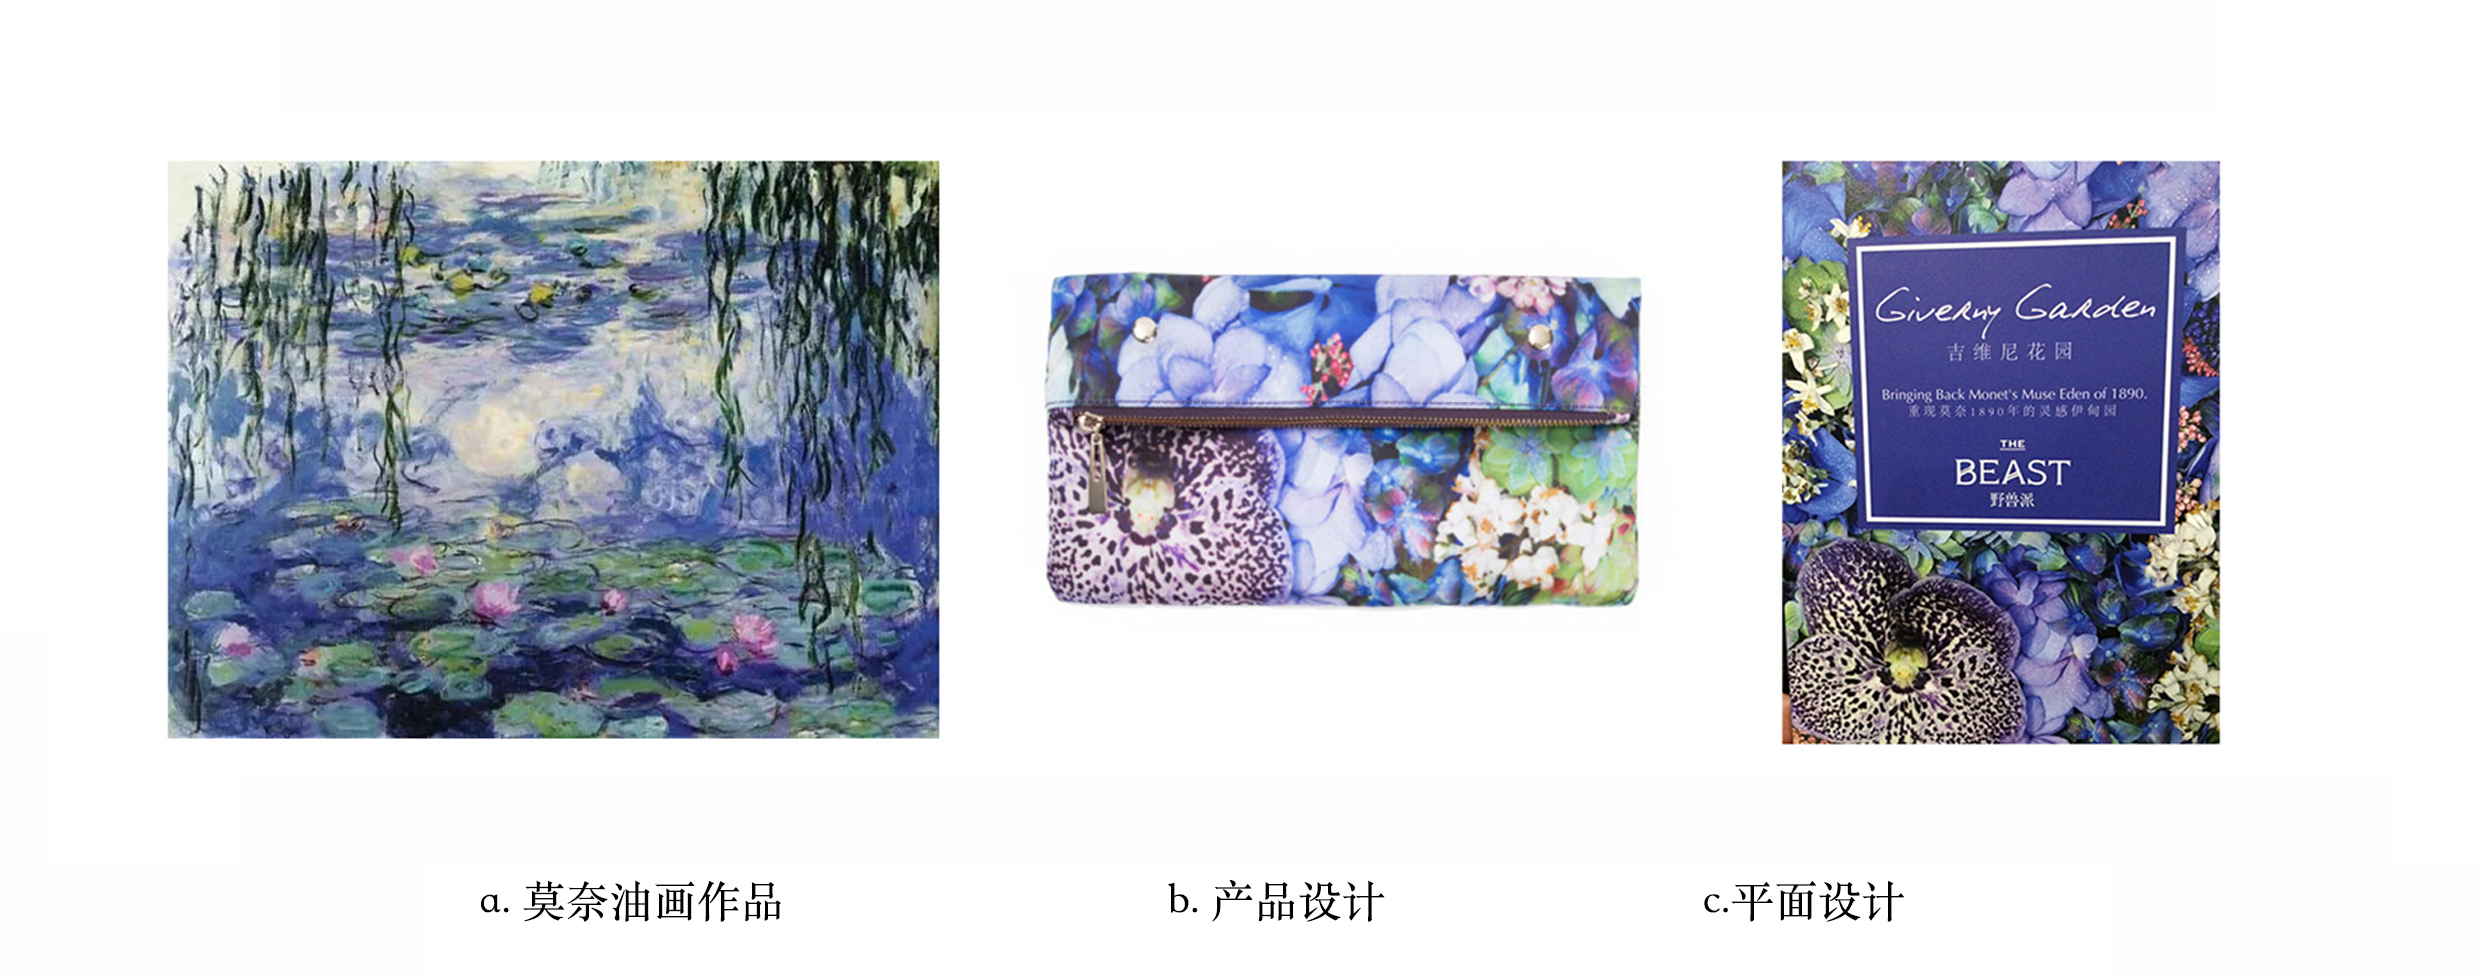
\includegraphics[width=\linewidth,keepaspectratio]{data/chapter-1/借鉴艺术品的设计.jpg}
\caption{从艺术品中借鉴色彩方案的设计作品}
\label{figure:从艺术品中借鉴色彩方案的设计作品}
\end{figure}

本文提出了一种基于语义智能理解的自动配色和上色系统。目前自动上色系统通常通过人工标注色彩、有限类型进行色彩填充或依赖已有色彩风格进行迁移,本系统通过从巨大的数据库中的艺术品学习,从艺术作品中提取色彩方案。依托艺术品图像和文本(包括介绍和题目)对应关系,使得系统直接智能地对人类的语言进行响应。实现根据文本输入来输出设计效果图的配色。

本文的实现方式如下:

1. 本系统依托艺术品交易数据库的内容进行机器学习和训练神经网络,对于数据库中的每一件艺术品有下列信息:艺术品的题目、类型、艺术品的文字描述、艺术品的图片(即绘画作品的内容),作者等。

2. 输入需求的文本描述,通过语义搜索的方式可以找出与之关联度高的艺术品文字及介绍,依托艺术品数据库中艺术品的的图像和文字介绍的匹配对应,即找出与输入文本关联度高的图片。

3. 从图片中提取色彩方案,包括绘画作品的色彩和配色比例。

4. 将提取的色彩方案运用到设计效果图上预览。上色使用泛洪填充算法(Flood Fill Algorithm)与随机游走(Random Walk)的方式,并且使用图层混合算法完成效果图的预览。

对于设计师而言,本系统可以将需求的文本描述即时转化为配色方案对设计线稿进行填充,方便的批量生成多个色彩方案以供选择,大大方便了其使用便捷性。

本文为了实现这个系统使用了三个创新点:1.使用了深度学习模型对语义进行理解;2.将图片信息与语义层面的隐藏信息进行关联,其图片风格相似性的偏序特性被保持到其语义描述的偏序特性中;3.本文使用了泛洪填充算法和随机游走的方式,对图像进行自动填充。

本文解决的难点一共有4点:1.使用word2vec对输入的文字、艺术品信息进行语义理解,设计带有语义信息的编码形式;2.输入文字编码信息与艺术品文本的编码信息对比,在数万条艺术品文本信息中搜索其中距离最近者;3.艺术品的色彩特征提取;4上色出现的一系列问题:色彩连续性、色彩比例等。

\section{本文结构安排}

本文为了实现基于语义智能理解的自动配色和上色,首先探索若干类似的课题:

之后本文详细的描述了系统的设计和实现过程。系统的整体结构从算法实现结构以及用户逻辑结构两方面设计。而系统的实现主要涉及自然语言处理,语义编码和搜索,色彩提取,上色四个方面。

最后展示该系统的的结果,通过输入语句案例进行测试,各类效果图测试案例测试该系统的理解能力、准确性、可用性、可拓展性。



%% !TEX root = ../main.tex

% 第一章一般名为绪论/引言,不可省略

\chapter{绪论}

\section{研究背景}

如何使计算机能够像人类一样思考、决策、行动这是人工智能科学家长久以来一直思考的问题。\cite{AIMD} 从20世纪六十年代, 科研工作者普遍关心的是如何利用计算机解决听觉、视觉、语言理解、自动推理等问题。 但是这些问题,尤其是计算机视觉和语音识别问题, 在相当长的一段时间内发展缓慢。 这是因为, 基于之前以分析为主的方法, 例如基于边缘检测等人工主观判断的特征进行图像识别, 或者利用语言学的专家知识进行语义理解和语音识别。 自从1987年, 卡内基梅隆大学李开复博士使用统计概率模型使得当时的语言识别技术大大提升, 使得人们开始注重利用统计学习模型进行人工智能相关问题的解决。 \cite{50_years_ai} \cite{manning2008introduction} \cite{abelson1985structure}

1986年, 时任加州大学圣地亚脑科学认知实验室的研究院Geoffery Hinton在Nature杂志上发表了一种利用反向传播(Back Propagation)自动优化神经网络模型的方法, 利用神经网络进行机器学习第二次成为机器学习研究的重点。 当时确实解决了一些复杂的问题, 例如1997年YaLeCun提出的卷积神经网络(Convolutional Neural Networks)能够识别手写的阿拉伯数字, 这在计算机尤其是人工智能领域是很重要的进步。 但是, 神经网络的参数多, 为了使得其参数收敛至稳定值, 需要大量的训练样本而且其巨大的矩阵运算是一般的计算机所不能承受的, 神经网络虽然有了一些优秀的表现, 但是并没有产生突破性的表现。 

2012年ImageNet计算机视觉识别比赛中,在加拿大蒙特利尔大学担任教授的Geoffery Hinton带领团队使得ImageNet图像识别的错误率由30\%以上下降到15\%一下, 这引起了轰动。 \cite{DBLP:journals/corr/abs-1301-3781} 
% htbp 什么的现在不要管
\begin{figure}[htbp]
    \centering  % 学位论文规定图表皆水平居中于版心 在 zjuthesis.cls 搜「版心设置」
    \includegraphics[width = .85\linewidth]{image_net_rank.png} % 设定图片宽度相对于版心宽度,图片文件资源名
    \caption{ImageNet 错误率的下降} % 图的题注
    \label{Russakovsky et al. arXiv, 2014} % 与 autoref 关联,设定交叉引用和显示「图x.x」
\end{figure}


从2012年之后, 深度学习这一机器学习范式, 被用来解决诸多问题。 例如此前的ImageNet下进行的计算机视觉比赛, 在2015年其识别的错误率已经低于人类的平均值。 2017年12月22日, 腾讯DPDAC NLP实验室使用深度学习神经网络训练的自然语言理解模型, 在机器阅读理解的比赛上的正确率已经达到81.790\%, 人类在这项测试中的评价准确率为\%82.304。 除计算机视觉和自然语言理解领域, 深度学习在决策领域也表现出了惊人的进步, 2017年10月, Google Deep Mind的AlphGo战胜了战胜了围棋世界排名第一的柯洁, 这表明深度学习在复杂决策上也是具有非常大的潜力。 

由于深度学习在计算机视觉、自然语言理解、决策等方面的突出表现。 科研工作者希望利用深度学习能够解决更加类似于人类的工作, 即 -- 艺术创作。 艺术创作长期以来被认为是人类独有的能力。 但是经过科学家们对于艺术创作过程以及艺术创作心理学的分析发现, 人类的艺术创作除了精神与心理学等生理原因, 其后天影响, 周围环境影响对艺术创作也是具有非常大的影响。 或者说, 创意, 创造力和后天学习具有密不可分的关系。 \cite{mq-zhanjian} \cite{adomavicius2005toward} \cite{gil2010state}


另外, 艺术创作在某些环境下也是重复的脑力活动, 例如在游戏音乐配乐, 游戏场景绘画, 电影场景绘画以及畅销书的写作等。 其重复的模式非常之多。 在此模型下, 艺术创作可以抽象为一个制作或者生成过程,如方程\eqref{eq:gene-art}所示。 

\begin{equation}\label{eq:gene-art}
ArtWork= Generator(f_0, f_1, f_2, \cdots, f_N, r_{x \sim p})
\end{equation} 

但是由于艺术生成具有区别于传统机器学习的两个特点, 第一是:其输出是一个序列性的而非特点长度的标签(Label)或者回归预测值; 第二是: 艺术的输入特征难以确定, 其输入也是一个复杂的序列过程。 例如音乐的生成依赖于诸多因素。 以上两个因素使得计算机进行自动艺术创作, 在长时间内依赖于规则,这使得计算机艺术创作不能广泛得适用于更加通用的场景。 

然而深度学习在特征自动学习(Representation Learning )和序列数据特征的提取中均具有良好的效果。 故,很多科研工作者开始使用深度学习相关的方法来尝试计算机自动生成艺术作品。 

除深度学习的背景, 《诗经》作为我国悠久的文化历史遗产。其最先即时用来歌唱的, 但是由于时间长远, 歌谱遗失。 如果能够利用现代技术为其自动谱曲, 那么将会为我国的古老艺术注入新的活力。 另外, 《诗经》虽然距离目前时代久远, 但是由于中国汉字的特点, 其大多数字义和意向与现在汉字的匹配度依然较高。 这给了使用现在歌词来恢复古老艺术的可能性。 第三, 诗经长度短小, 序列模型的长依赖问题对其影响不大, 所以也减轻了模型的训练难度。 

基于以上背景, 本文研究一种利用深度学习的理论和方法, 自动依据歌词生成音乐的方法。 并且探讨如何将其应用到诗经中。 本文提出了一种能够解决此问题的模型并使用真实数据进行了实验, 表明了该模型的有效性。 


\section{国内外研究现状}

因为本研究课题是机器学习、自然语言处理和音乐合成的交叉领域, 本小节主要从以下三方面进行国内外现状的分析: 

\begin{enumerate}

	\item 自动音乐生成
	\item 表示学习 (Representation Learning)
	\item 序列化生成 
	
\end{enumerate}

\subparagraph{计算机自动音乐生成} 实现计算机自动谱曲或者自动音乐合成不同的科研工作者使用了很不相同的方法。 考虑的范围从语法和词法等语言学知识, 到自动决策等人工智能领域的知识以及复杂系统建模等均有涉及。 目前涉及到的方法如下: 

\begin{itemize}

	\item 语言学方法
	\item 符号系统
	\item 马尔可夫链
	\item 机器学习与人工智能方法
	\item 原细胞有限自动机
	\item 基于规则的算法 [Wiggins(1991), Nierhaus(2009)]
	
\end{itemize}

%除使用以上方法, 目前仍有人工定义负责算法进行音乐的自动合成, 例如Wiggins(1991), Nierhaus(2009)。 

本文主要关注机器学习与人工智能方法的研究现状。 使用人工智能方法进行计算机自动谱曲首先提出在20世纪80年代. 1989年, Todd首先利用三层神经网络进行训练。 基于一系列初始的配置信息及已有的乐谱, 神经网络通过学习能够依据特定的配置信息(Configuration)生成特定的音高(pitch)。之后1989年, Duff使用巴赫的音乐进行训练, 是的计算机能够自动产生巴赫风格的音乐。 以上两个人使用的都是循环神经网络(Recurrent Neural Networks)。 

为了解决更加复杂的音乐合成问题, 例如节奏、旋律、和弦等, 一些研究者在人工神经网络的基础知识提出了混合系统, 即将神经网络与其他系统向结合。\cite{DBLP:ALYSIA} 较为著名的是NETNEG(Goldman et al)首先使用一个六层的神经网络产生基本的旋律片段, 然后使用基于音乐理论的规则构成的系统, 将其构成更为复杂的音乐。 该基于音乐理论的规则系统主要用于解决不同旋律之间的衔接问题。 2004年, 结合了神经网络与马尔科夫随机过程的模型被提出(Verbeurgt el al 2004)。 之后, 在2011年, Coca 等人利用神经网络加伪随机过程, 合成了能够合成较为复杂的音乐。 除此之外, 使用非监督方法也是存在的。 Burton(1998)年提出了一种生成算法模型, 首先他使用矩阵对音乐的特征进行表示, 其次其使用和弦理论,使用神经网络对不同特征进行距离。 经过这样的过程, Burton能够生成若干簇符合和弦美感的音乐。 在2007年, Phon-Amnuaisuk 等学者提出了一种新的方法。 通过音乐的自适应对应(self-organizing map)能够产生和之前所熟悉的一些音乐。 与监督学习不同的是, 该方法在产生音乐时, 并不需要训练数据。 

以上所讲述的所以生成音乐的方式全部都是面向自动产生音乐的, 使用歌词生成音乐并不如利用歌词生成音乐普遍。 Monteith等人利用已知的音乐知识, 编制了基于规则的音乐产生模型, 其通过输入文字的文字特征能够产生特定的音乐。 2016年, 加州大学圣地亚哥的Margareta Ackerman提出了一种基于随机森林的全自动音乐生成模型, 其输入为歌词, 输出为歌曲的节奏和音高(scala degree)。 虽然其模型训练结果的准确度较高, 其节奏预测的准确率达到了86.79\%, 其音高的预测准确率达到了72.28\%。 但是该模型显然有以下三个问题: 

\begin{enumerate}

\item{人工构建特征}: 该模型由人工自定义了16个特征, 包括了时间元素, 音高, 单词频率等各种。 由于人工选择特征, 不可避免的会受到人工的先验知识的影响, 并不能挖掘出深层次的范式; 
\item{训练数据过小}: 其论文使用的是24首歌进行训练, 显然该论文是音乐自动作曲的一次尝试,该结果并不能产生良好的泛化效果;
\item{输出噪声多}: 虽然该论文模型的准确率高, 但是音乐不同于其他通常的数据, 其主要在于和谐, 虽然该模型在音高上有72.28\%的准确率, 但是由于个别异常值的影响, 使得整个音乐并不具有美感。 

\end{enumerate}

但是不可否认的是, 该论文为之后利用计算机依据歌词自动生成提供了指导意义。 


\subparagraph{表示学习与Embedding} 表示学习是机器学习中重要的研究内容, 主要研究如何将数据有效的表示到计算机中。 其中, 最重要的的方式是如何通过一种方式使得新表现的数据形式能够保持其原始线性关系\cite{embedding}, 这种行为在计算机及数学中叫做embedding。Embedding是指,保持一种偏序关系,是的我们已知的某种关系也保持到新的向量空间中。 Embedding的具体定义如下:

$$ \forall x_{1},x_{2}\in X:x_{1}\leq x_{2}\Leftrightarrow F(x_{1})\leq F(x_{2}). $$


例如,之前人们对自然语言进行计算的时候, 使用的表示方式多是one-hot方法表示单词或者利用tf-idf等信息表示一句话。 但是这种表示并不能表征有效的表征句意。 Mikolov 等科学家使用的word2vec, 使得我们能够获得更加深层次的语义 \cite{DBLP:journals/corr/abs-1301-3781}。 由于word2vec保持了词汇意思的线性关系, 使得我们利用已知的单词获得新的,意思解决的单词变成了可能。 在Mikolov提出了Skip-Gram和CBOW等word Embedding的方法之后, 斯坦福大学NLP组提出的Glove,以及Salesforce提出的ContexVec \cite{DBLP:journals/corr/abs-1708-00107} 都获得更加良好的表现。 


\begin{figure}[htbp]
    \centering  % 学位论文规定图表皆水平居中于版心 在 zjuthesis.cls 搜「版心设置」
    \includegraphics[width = .85\linewidth]{word2vec2.png} % 设定图片宽度相对于版心宽度,图片文件资源名
    \caption{Word Embedding 对单词词义的线性保持} % 图的题注
    \label{word2vec} % 与 autoref 关联,设定交叉引用和显示「图x.x」
\end{figure}

本文借鉴 word embedding 的思想,对音乐元素进行embedding, 这样做的好处是, 将以前的88个音乐元素扩展至用户可自定义的个数个音乐元素(依照训练数据的不同, 该自定义元素数字可从几千至几十万), 这些音乐元素经过embedding, 可使得具有类似情感,类似表达的音乐元素进行聚类。 让计算机把音乐元素当做88个单独的元素看待类似于让计算机把所有的英文文本当做26个字母看待。 经过以上关于word embdding的分析, 这显然是低效的。 如果能够让计算机自动发现类似于单词的音乐元素词组, 将能够大大提示模型的抽象能力与泛化能力。 

\subparagraph{序列化生成} 传统的机器学习模型能够处理的是输出定长的数据输出定长的预测结果。 如何使得机器学习模型能够接受边长的输入产出边长的输出, 此问题直到2014年由Google的科学家 Sutskever 等人在进行机器自动翻译模型研究时提出了Seq2Seq模型才获得了比较良好的改进 \cite{DBLP:journals/corr/SutskeverVL14}。 之后,  Bahdanau 等人又实现了在Seq2Seq模型中增加了注意力机制(Attention), 使得计算机能够接受变长输入, 输入变长的数据。 Seq2Seq以及Attention机制,使得机器翻译的水平有了大幅度的提示。 其次, Seq2Seq 也被用于自动作画, 自动生成段文字等领域。  所以本文参照机器翻译的模型, 将计算机依据歌词自动合成音乐的问题抽象为机器自动翻译的问题。


\section{论文研究内容}

文论文主要研究以下内容:

\begin{itemize}

	\item{如何获得大量的音乐训练数据}
	\item{如何高效的进行音乐元素的embedding}
	\item{如何构建序列生成模型}
	\item{如何将模型迁移适应到古代诗歌风格}

\end{itemize}

\subparagraph{如何获得大量的音乐训练数据}

利用深度学习进行序列生成首先需要解决的是大量训练数据的问题。但是面临的问题是,目前的音乐文件大多都是受版权保护的, 不能像ImageNet或者语音识别等领域具有大量的训练数据。 但是本文利用以下两种方式进行训练集的扩展: 1. 利用N-Gram以及随机skip的方式, 可能让训练数据集增加一个数量级(本文测试结果为15倍);2. 利用word embedding获得的同义词、近义词词组, 对文本进行随机替换, 可以将训练集继续增加, 增加接近一个数量级(本文实验结果为0.7倍)。经过以上两种方式, 可以将训练数据扩大两个数量级。 在下载1000首歌曲的情况下, 可以生产10万条训练记录, 基本上达到了深度学习能够利用的数据量。   

\subparagraph{如何高效的进行音乐元素的embedding}

为了更加高效的对音乐元素进行表征,本文借鉴word embedding的方式对音乐元素进行embedding。 经过这样的处理, 可以将目前常见的88个音乐元素变成更多的, 能包含具体意向、情感特征的音乐元素。 对于音乐元素单独的处理, 除了能够依据音高表示每个元素不同以外并不能包含其他的特征,但是如果能够发现更加丰富的音乐元素表示特征, 则会大大增加模型的表现能力。 也能够在情感、语义层面对其进行扩展和分析。 

但是进行高效的embedding是复杂的。 首先需要对音乐数据进行离散化处理, 虽然音乐的乐谱表现为离散值, 但是对于人类的感触是连续值。 首先需要考虑如何将音乐进行有效的离散处理。 其次是embedding时候网络结构的选择及其训练模型的定义, 网络结构如何选择, Loss函数如何定义, 这些都是本文需要考虑的问题; 第三是embedding的维度, 因为如果embedding的维度过大, 就不能在有限的数据集下收敛到到全局最优解, 如果embedding的维度过小, 就会迅速收敛到局部最小值。


\subparagraph{如何构建序列生成模型}

如何将Seq2Seq的思想利用该课题中, 即已知歌词生成乐曲, 这是本文需要解决的一个难点。 我们知道,同样的歌词可以配以不同的音乐,而同样的音乐也可以配以诸多的歌词。 例如陕北的“信天游”, 几乎所有的歌词都是一种配乐。 这就说明歌词和乐曲直接的映射关系是一种若映射, 那如何将这种弱映射关系利用模型学习出来, 是本文研究的重点。 

依据歌词生成乐曲,是不是一个可学的问题, 如果是可学的, 如何定义网络模型使得该范式可以被模型泛化, 如果不可学, 如何增加必要的辅助内容使得该范式可学, 这都是本文需要重点考虑的问题。 


\subparagraph{如何将模型迁移适应到古代诗歌风格}

本文最后采用诗经作为歌词输入,利用计算机自动为其谱曲, 但是这个具有两个问题: 一、诗经的语言形式和表现内容和用以训练的数据具有很大的不同, 如何使得模型能够适应这种语言内容, 这是需要研究的; 第二、诗经的风、雅、颂等依据史书记载, 是不同风格的。 如何做到同样类别的音乐具有类似的音乐表现, 这也是需要解决的一个难点。 

本文通过借鉴迁移学习(Transfer Learning)在计算机视觉上的成功, 在训练的Seq2Seq模型基础上对该模型进行迁移。 使模型迁移到能够适应于中国古风、诗歌;第二, 通过文本挖掘、文本分类的方法, 将不同音乐元素进行距离, 然后自动有模型得出不同音乐类型的音乐元素的分布。 之后借鉴CGAN(Conditional
 Generative Adversarial Networks)的方法, 为网络模型提供一个初始的依赖值, 通过改值用来调整音乐的美学特征。 

\section{论文组织结构}

%简明扼要的介绍下各章主旨,版面控制半页内。

\begin{itemize}

\item 第二章 \textbf{音乐元素的表征和embedding}

第二章主要解决如何将音乐元素进行有效的表征和embedding, 主要涉及到音乐元素的离散化、正则化以及标准化。 这是使得模型能够有效利用数据进行结果输出。 

\item 第三章 \textbf{歌词词向量的构建}

第三章主要利用word2vec的方法将所有的歌词进行向量化, 这是模型能够有效的使用输入训练数据进行学习。

\item 第四章 \textbf{训练数据的生成}

依据前文生成的音乐向量以及词向量, 可以此基础之上构建训练数据。 通过N-Gram滑窗, Skip-Gram随机跳跃, 以及利用word2vec结果进行同义词替换等方法, 使得模型获得了大量的训练数据。 


\item 第五章 \textbf{计算机序列生成模型的构建}

此章研究使用Seq2Seq进行序列生成的原因以及如何将Seq2Seq利用到该课题中。 主要解决此问题范式是否为可学习、可训练的问题, 以及如何使得该问题变成可学习,可训练的问题。 如何设计网络结构,层级结构, 如何选择神经元, 如何设计Loss函数, 如何设计输出输入格式, 使得该模型可训练。 

\item 第六章 \textbf{系统模型实现与结果分析}

通过网易云音乐下载的1000首歌曲, 以及通过编写网络爬虫从网络中获取到的这1000首歌曲匹配的歌词。 在此模型上进行训练,观察实验结果。 并且通过对训练结过程及结果的分析, 获得此模型的学习能力及泛化效果。 

%\item 第七章 \textbf{针对《诗经》的迁移训练}

%此章讨论如何利用迁移学习将此模型迁移到适用于《诗经》的歌曲生成中。 

\item 第七章 \textbf{总结分析}

此章讨论了此模型的优点和存在的问题, 以及提出了对未来的展望。 

\end{itemize}

\chapter{技术路线、现有方法分析及背景支持}

\section{技术路线分析}

事实上,承上一章所述之背景,设计工作和艺术创作虽然强烈依赖作者的感受力和创造性,但是在某些环境下也是重复的脑力活动。例如在游戏美术、电影场景绘画、高概念电影故事创作以及网络小说的写作等工作中,创作常常符合某种模式,其重复的模式非常多。在此模型下,艺术创作可以抽象为一个制作或者生成过程,如方程\eqref{eq:gene-art}所示。 

\begin{equation}\label{eq:gene-art}
ArtWork= Generator(f_0, f_1, f_2, \cdots, f_N, r_{x \sim p})
\end{equation} 

但是由于传统机器学习的两个特点,使得艺术生成并不适用传统机器学习的方法,第一是:其输出是一个序列性的而非特点长度的标签(Label)或者回归预测值; 第二是: 艺术的输入特征难以确定, 其输入也是一个复杂的序列过程。这两个因素使得计算机进行自动艺术创作在长时间内仍然依赖于人类编写规则,使得计算机艺术创作不能广泛得适用于更加通用的场景。 

而深度学习在特征自动学习(Representation Learning )和序列数据特征的提取中均具有良好的效果,所以很多科研工作者开始使用深度学习相关的方法来尝试计算机自动生成艺术作品。 

色彩方案设计是在设计领域中普遍的一个工作方式。作为一个设计师,在每个项目中,选取合适的配色方案是一个重要的工作。在设计师设计的过程中,例如设计服饰,软装设计,建筑外观设计等,依据现有的环境特点,应用场景,目标用户,需要制定配色方案,然后将配色方案应用于整体方案上,有时配色方案还会应用到成套的产品中的各个子产品。由于自然语言理解与图像识别等领域目前都有了长足的进步,所以设计作品自动配色这个问题目前有可能使用神经网络和深度学习的内容进行自动化。 

而且,由于自然语言理解在最近几年取得的成果,其在语义理解方面可以良好的应用于设计作品自动配色这样领域。目前,计算机辅助设计在这方面的方式是采用一张配色表,使用关键词进行配色,例如图 \ref{img:peise} 这种方式进行。 这种方式其实是计算机语言理解的时候的一种折中做法。 

\begin{figure}[htbp]
    \centering  % 学位论文规定图表皆水平居中于版心 在 zjuthesis.cls 搜「版心设置」
    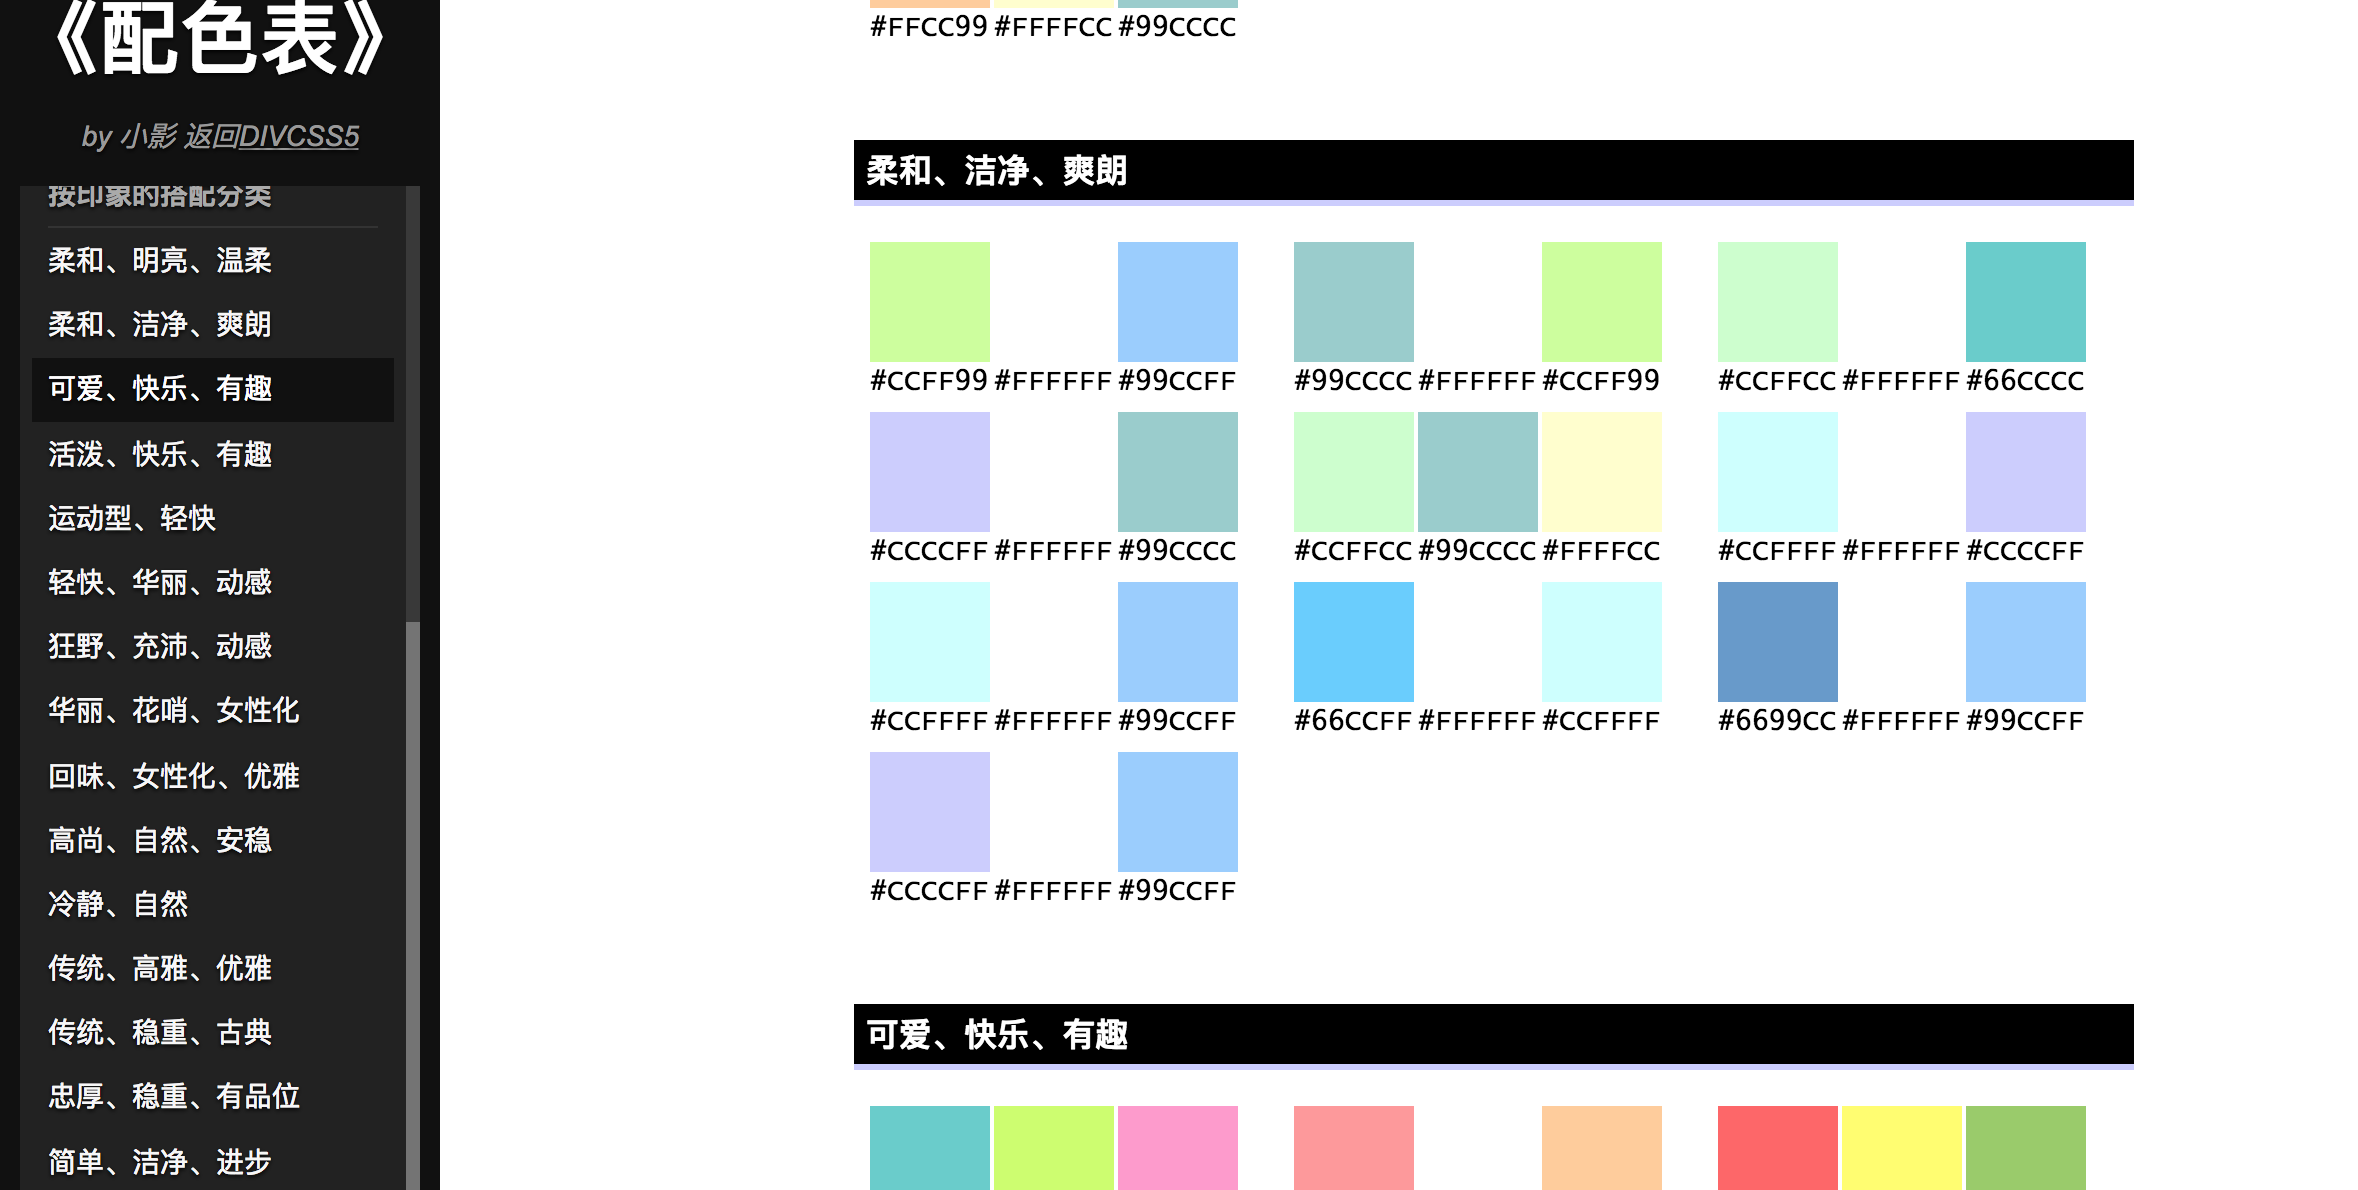
\includegraphics[width = .55\linewidth]{data/chapter-2/peisebiao.png} % 设定图片宽度相对于版心宽度,图片文件资源名
    \caption{设计师使用配色表进行配色} % 图的题注
    \label{img:peise} % 与 autoref 关联,设定交叉引用和显示「图x.x」
\end{figure}

这种方式存在两个问题:第一, 有限的词汇其实不能表达丰富的含义,设计作品的应用涵盖生活的方方面面, 其需要表达的语义丰富性是远远高于有限的这些单词的; 第二,单个词汇与整体意向组织不具备线性叠加的关系。 即, 设计师要设计出一个“温柔的春天”这样意境的设计作品, 其颜色不能是先选择“温柔”, 再选择“春天”, 而是需要再次进行加工。 将这两种的意向进行重叠。 而这种加工是目前的配色表不能完成的。 

因此, 本课题希望基于目前的自然语言理解的技术与图像自动化处理的方式, 实现从作者的直接描述到自动产生配色图的自动化转化。 例如, 一个设计师接到了室内软装设计的需求, 甲方的需求是\textbf{“洋溢着春天的感觉, 要很温柔, 然后要像有小孩在草坪上奔跑一样”}, 本课题要实现的基于语义识别的自动配色系统,只需要将这句话\textbf{“洋溢着春天的感觉, 要很温柔, 然后要像有小孩在草坪上奔跑一样”},输入到系统中,就会自动匹配色彩方案,并且可以为直接其线稿进行上色,可以方便的预览,把握整体风格,参考及其方便,甚至批量生成预览图像,为客户展示和预览也节省大量时间。

基于之上的分析,本课题研究一种例如深度学习与表示学习的方式,在此基础上实现从语言理解到色彩搭配的自动转化。之后,本课题在真实数据库上进行了实验,本模型确实能够实现良好的自动化转化,证明了该模型的有效性。 


\section{国内外研究现状}

因为本研究课题是机器学习、自然语言处理和图像合成的交叉领域, 本小节主要从以下三方面进行国内外现状的分析: 

\begin{enumerate}

	\item 自动图像合成
	\item 表示学习 (Representation Learning)
	\item 序列化生成 
	
\end{enumerate}


\subsection{计算机自动图像生成} 实现计算机自动图像生成或自动色彩搭配,目前涉及到的方法如下: 

\begin{itemize}

	\item 查表法
	\item 马尔可夫链
	\item 机器学习与人工智能方法
	\item 原细胞有限自动机
	\item 基于规则的算法 [Wiggins(1991), Nierhaus(2009)]
	
\end{itemize}

%除使用以上方法, 目前仍有人工定义负责算法进行音乐的自动合成, 例如Wiggins(1991), Nierhaus(2009)。 

使用机器学习与人工智能方法主要分为两个类型, 一是监督式的(Supervised), 希望给计算机一定的监督样本(Samples), 使得计算机能够拟合一个函数, 使得该函数能够拟合训练数据到已知样本标签的映射如等式 \eqref{eq:map}

\begin{equation}\label{eq:map}
function(x) \rightarrow y
\end{equation}

监督式的学习方式在图像生成领域应用不多, 主要使用因为该种方式主要应用在问题结果确定已知并且有限的情况下, 即 其目标函数的$y in \mathbf{R}^n$ 且 $|y| <= N$ 。 但是, 在图像生成领域,目标函数的结果大家的期望并不是从已知的范围内选择一些出来,而是希望能够自动创作。 

所以目前机器学习方式主要采用\textbf{非监督学习}的方式进行图像生成。 非监督的学习方式主要通过从已知的信息中, 获得不同类型的信息、数据的隐含关系, 例如图 \ref{img:unsupervised}。 

\begin{figure}[htbp]
    \centering 
    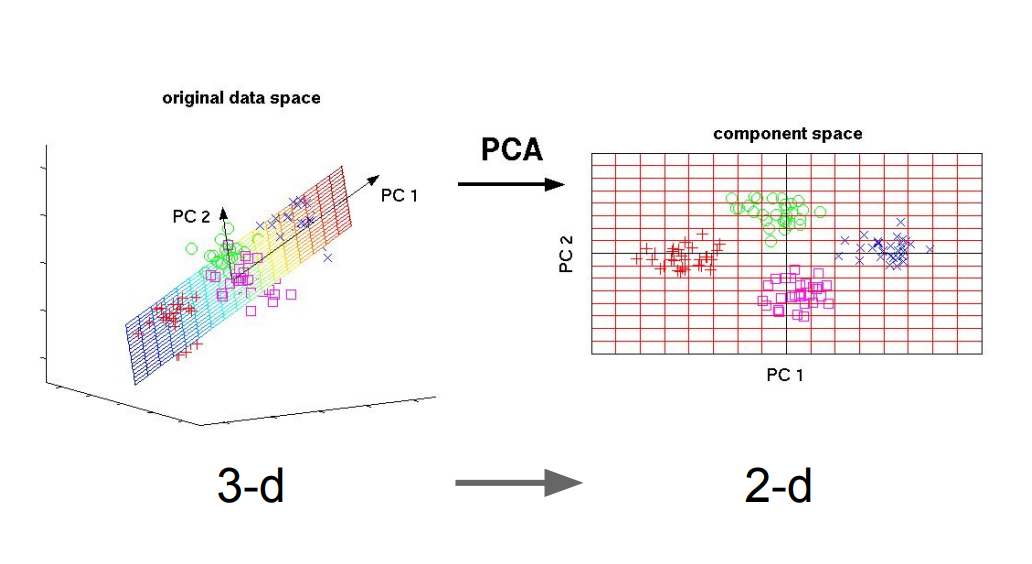
\includegraphics[width = .55\linewidth]{data/chapter-2/unsupervised.png} 
    \caption{非监督式学习主要用来找到影藏的关系} 
    \label{img:unsupervised} 
\end{figure}

而基于非监督式的学习, 提出的Autoencoder 自编码模型可以在缺少某些信息的情况下, 对图像进行重建。 例如图 \ref{img:autoencoder} 所示。

\begin{figure}[htbp]
    \centering  
    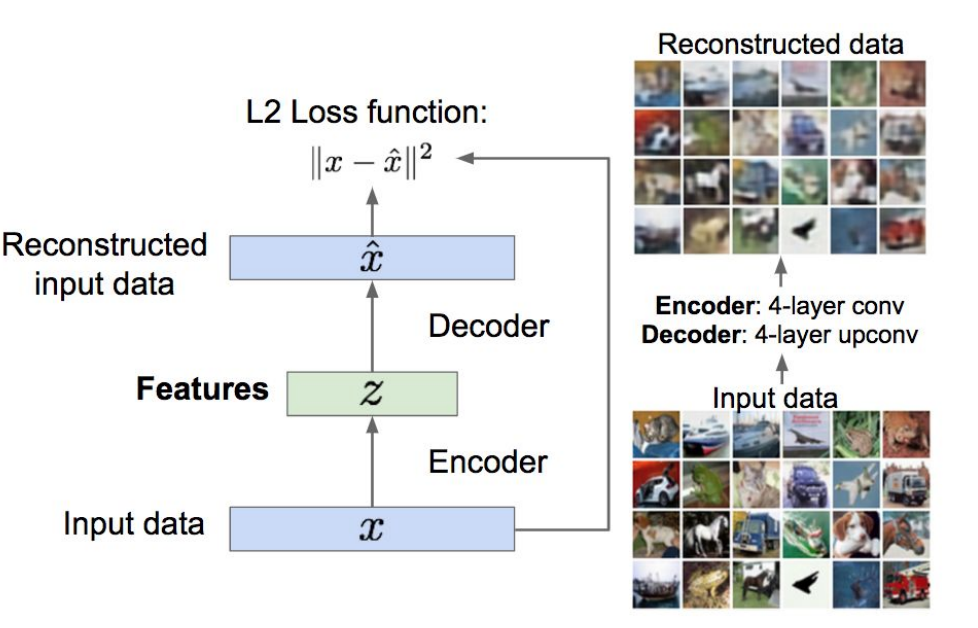
\includegraphics[width = .55\linewidth]{data/chapter-2/autoencoder.png} 
    \caption{自编码模型可以从缺少的信息中重建图片} 
    \label{img:autoencoder} 
\end{figure}

由于重建信息的成功, 如图 \ref{img:autoencoder}, 科研人员考虑如何通过已知的数据, 获得其潜在的数据概率分布, 从而可以不依靠部分信息而对全部的信息进行重建, 以重建其具备与源数据源具有同样数据分布的数据。 

\begin{figure}[htbp]
    \centering  
    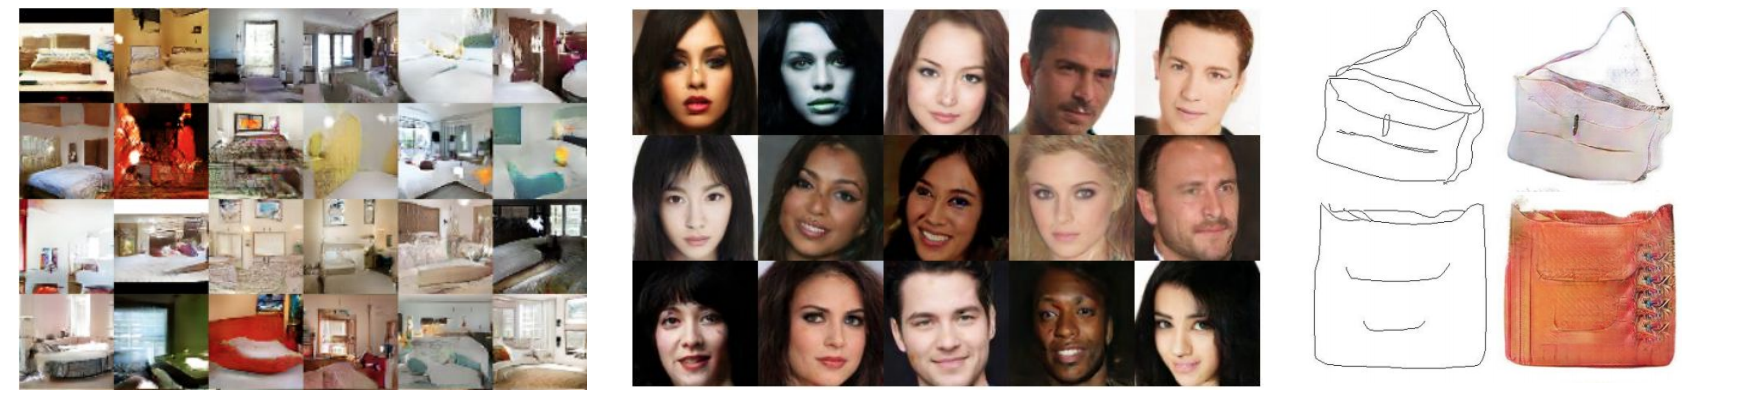
\includegraphics[width = .55\linewidth]{data/chapter-2/gene.png} 
    \caption{生成模型可以直接生成新的信息而不基于输入的部分信息} 
    \label{img:gene} 
\end{figure}

要完成此任务, 目前主流的使用PixelRNN/CNN, GAN,马尔科夫连, 以及模仿学习(Imitation Learning), 这些模型都可以模型训练之后, 不需要输入部分“初始信息”, 而直接获得新的符合原来数据分布的新数据, 例如图 \ref{img:gene} 所示, 模型可以随机的产生室内的图片, 人像, 以及自动为线稿配色。  



\subparagraph{计算机生成图像——GAN} 随着理论研究的发展,计算机艺术辅助工具也有了新的突破,通过对抗神经网络算法(Generative adversarial networks - GAN),能够自动生产图片。\cite{radford2015unsupervised},GAN由判别器和生成器实现,判别器对照相机拍的照片和生成器生成的图像进行分类,而生成器从随机噪声中生成尽可能以假乱真的图像,判别器和生成器相互对抗,最后生成判别器无法判别的图像。这种模型,可以生成现实风格的图像,也可以用于将马赛克还原为清晰的照片。使用GAN可以根据文字生成图片,如图~\ref{figure:GAN}。\cite{goodfellow2014generative} \cite{mcaleergenerative}

\begin{figure}[!htbp]
\centering

\includegraphics[width=\linewidth,keepaspectratio]{data/chapter-1/gan.jpeg}
\caption{GAN从文字生成真实的图片}
\label{figure:GAN}
\end{figure}

图~\ref{figure:GAN}中显示基于GAN可以根据一句话,例如“小鸟,胸部和冠羽是粉红色的,黑色的一级和次级飞羽”就可以生成类似照片的图片。使用“胸部和冠羽是粉红色的鸟”和“黑色飞羽的鸟”的照片作为真实照片进行训练,生成器生成尽可能以假乱真的图像,判别器对真实照片和生成器生成的图像进行分类,相互对抗,最后生成判别器无法判别的图像。于是生成器就可以生成满足“小鸟,胸部和冠羽是粉红色的,黑色的一级和次级飞羽”这句话的图片。GAN生成的图片非常真实,但是每每面对新的一句话,它就需要大量的图片和较长的时间训练GAN模型。

\subparagraph{自动配色的探索}pixel2pixel相关的工作中也有关于配色选取的工作。colormind使用pix2pix的方式从输入照片提取生成色彩方案。\cite{pix2pix2016}\cite{chen2015improved}与此同时也有研究者研究通过大数据探讨关于配色的问题,多伦多大学的Peter O'Donovan等人通过color.adobe.com、www.coluorlover.com等配色网站上用户对各类配色的打分数据,使用机器学习的方式学习为色彩的和谐程度打分。\cite{O'Donovan:2011:CCL:2010324.1964958}

\begin{figure}[!htbp]
\centering
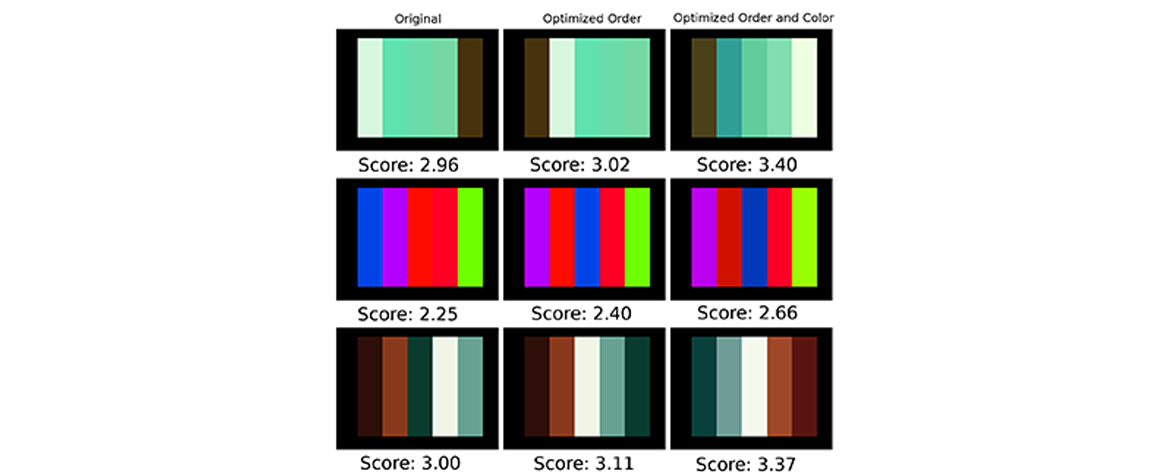
\includegraphics[width=\linewidth,keepaspectratio]{data/chapter-1/Color Compatibility.png}
\caption{从大量图片中学习色彩和谐程度}
\label{figure:Color Compatibility}
\end{figure}


\subparagraph{自动上色}

pixel2pixel探讨了更多基于对抗神经网络的,从图像生成图像的应用。在这一系列的相关工作中,包括能够为黑白照片自动上现实的合理的颜色,也可以为轮廓填充现实的合理颜色,以及从符号化的色块表达生成现实风格的图片,自动生成遮罩,自动替换照片中的人物。\cite{deng2010binary}

\begin{figure}[!htbp]
\centering
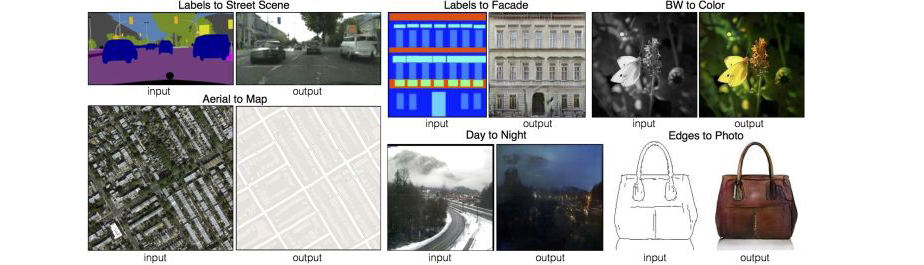
\includegraphics[width=\linewidth,keepaspectratio]{data/chapter-1/pix2pix.jpg}
\caption{pixel2pixel的若干应用}
\label{figure:Manga Colorization}
\end{figure}

有若干的项目都在讨论关于日本式漫画的自动上色问题,例如PaintsChainer和 Manga Colorization,如图~\ref{figure:Manga Colorization}。\cite{Qu:2006:MC:1141911.1142017} \cite{DBLP:journals/corr/ZhangJL17} 日式漫画风格较为统一,图形基本封闭,模式较为固定,并且对批量上色要求巨大。Manga Colorization能在标注颜色的情况下为二次元图片自动上色。PaintsChainer不局限于封闭的图形,并且自动完成上色与阴影模式,但其就效果而言,常常出现不可控的色块和理解错误的内容。

\begin{figure}[!htbp]
\centering
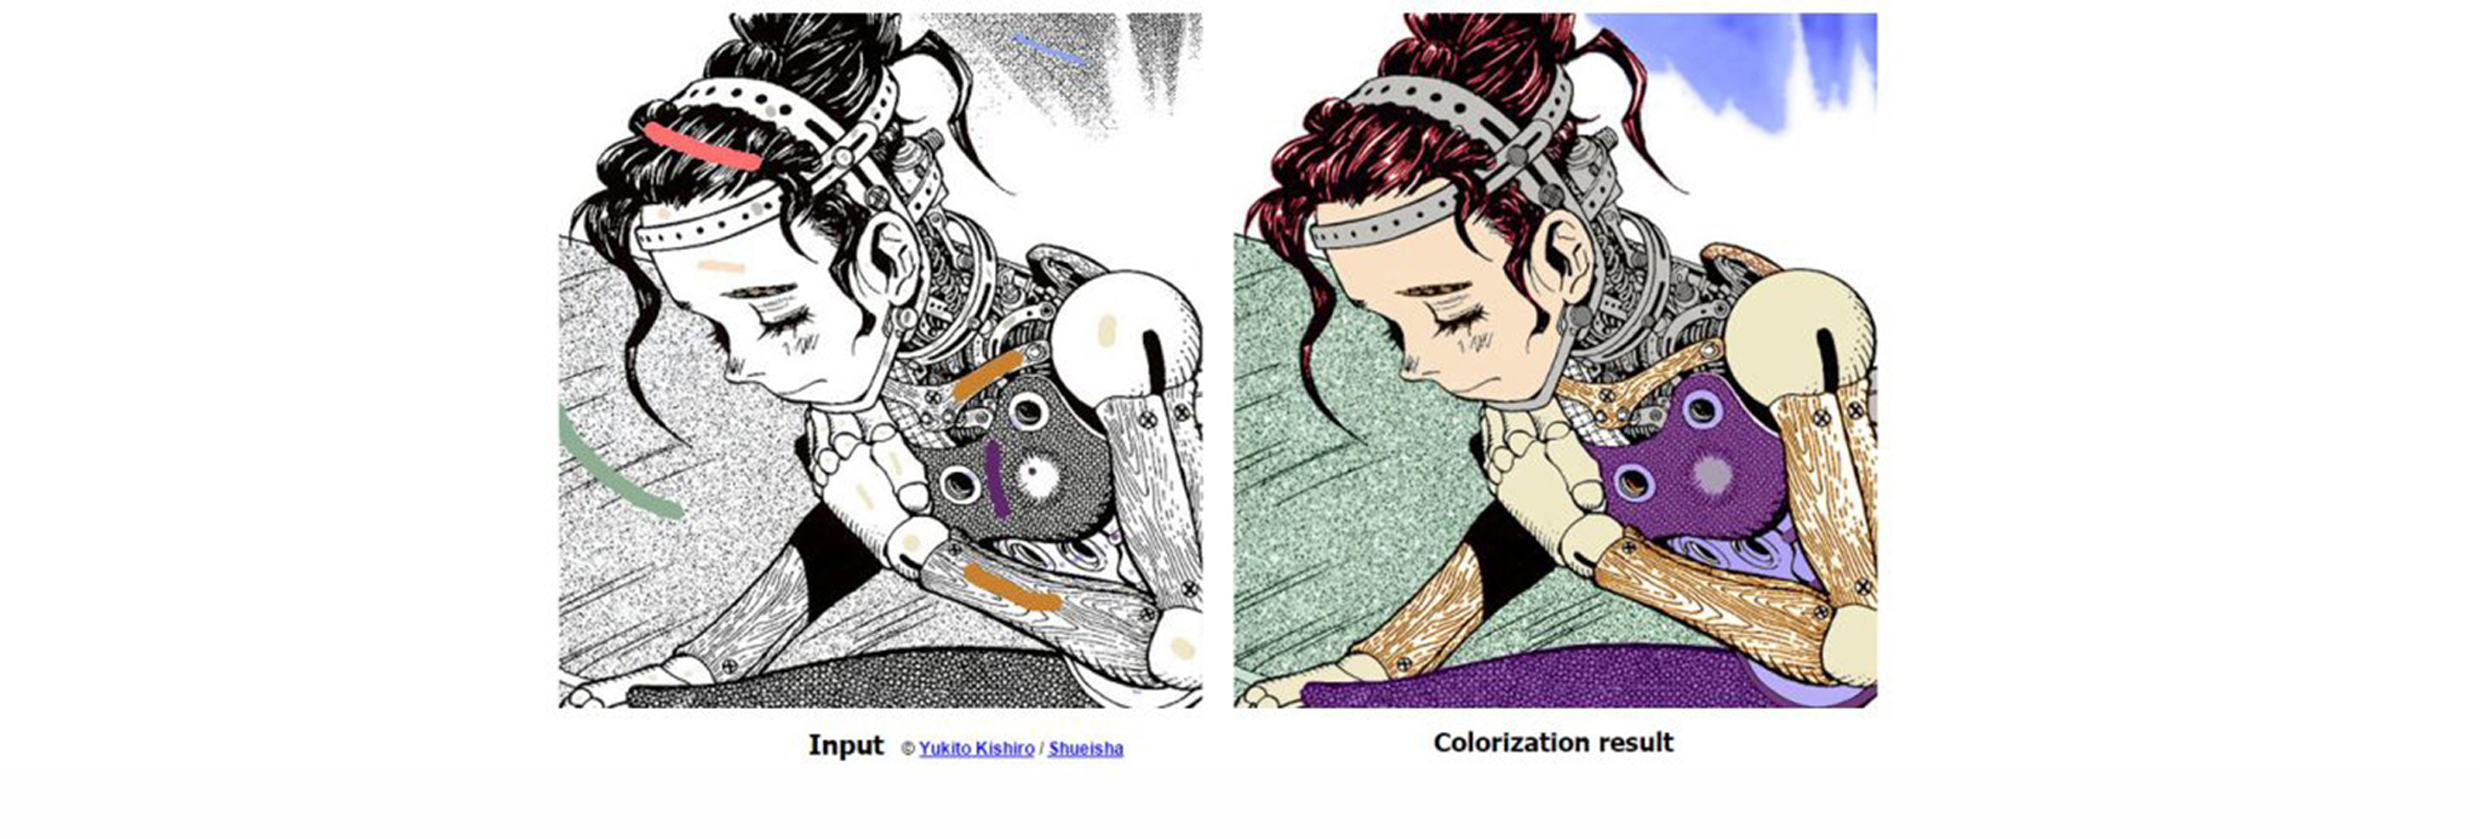
\includegraphics[width=\linewidth,keepaspectratio]{data/chapter-1/Manga.jpg}
\caption{Manga Colorization在标注颜色的情况下为二次元图片自动上色}
\label{figure:Manga Colorization}
\end{figure}

\subsection{表示学习与Embedding} 

表示学习是机器学习中重要的研究内容, 主要研究如何将数据有效的表示到计算机中。 其中, 最重要的的方式是如何通过一种方式使得新表现的数据形式能够保持其原始线性关系\cite{embedding}, 这种行为在计算机及数学中叫做embedding。Embedding是指,保持一种偏序关系,是的我们已知的某种关系也保持到新的向量空间中。 Embedding的具体定义如下:

$$ \forall x_{1},x_{2}\in X:x_{1}\leq x_{2}\Leftrightarrow F(x_{1})\leq F(x_{2}). $$


例如,之前人们对自然语言进行计算的时候, 使用的表示方式多是one-hot方法表示单词或者利用tf-idf等信息表示一句话。 但是这种表示并不能表征有效的表征句意。 Mikolov 等科学家使用的word2vec, 使得我们能够获得更加深层次的语义 \cite{DBLP:journals/corr/abs-1301-3781}。 由于word2vec保持了词汇意思的线性关系, 使得我们利用已知的单词获得新的,意思解决的单词变成了可能。 在Mikolov提出了Skip-Gram和CBOW等word Embedding的方法之后, 斯坦福大学NLP组提出的Glove,以及Salesforce提出的ContexVec \cite{DBLP:journals/corr/abs-1708-00107} 都获得更加良好的表现。 


\begin{figure}[htbp]
    \centering  
    \includegraphics[width = .85\linewidth]{data/chapter-2/word2vec2.png} 
    \caption{Word Embedding 对单词词义的线性保持} 
    \label{word2vec} 
\end{figure}

\subsection{序列化生成:PixelRNN/CNN}

\begin{equation}\label{eq:pix}
p(x) = \prod_{i=n}^{n} p(x_i|x1, ..., x_{i-1})
\end{equation}

该模型基于一个信念网络(Belief network) \eqref{eq:pix}, 其中, $ p(x) $ 是某图像 $x$ 的似然分布, 而 $pr(x_i|x_1, ..., x_{i-1}$ 是某个像素的概率在给定该像素之前的所以像素分布之下的条件概率。 该信念网络希望通过网络模型获得其条件概率的最大分布。 要生成一个像素 pixel 需要获得上一个 pixel的值, 通过一个RNN或者CNN网络, 实现序列化的生成, 如图 \ref{img:pix-matrix} 所示。 

\begin{figure}[htbp]
    \centering 
    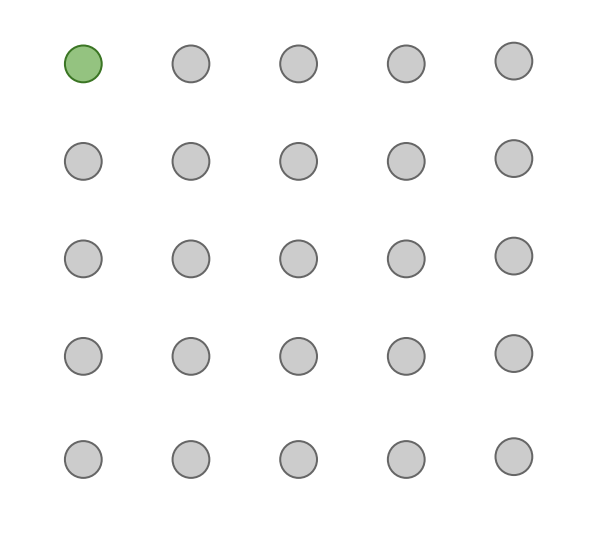
\includegraphics[width = .55\linewidth]{data/chapter-2/pixel_matrix.png} 
    \caption{pixel network 通过序列化的像素生成图像} 
    \label{img:pix-matrix} 
\end{figure}

依照此模型, 可以自动生成图像, 例如图 \ref{img:pix-example} 所示, 该模型在进行CFAIR10和ImageNet数据库的训练之后, 能够随机生成与之类似的图形. 

\begin{figure}[htbp]
    \centering  % 学位论文规定图表皆水平居中于版心 在 zjuthesis.cls 搜「版心设置」
    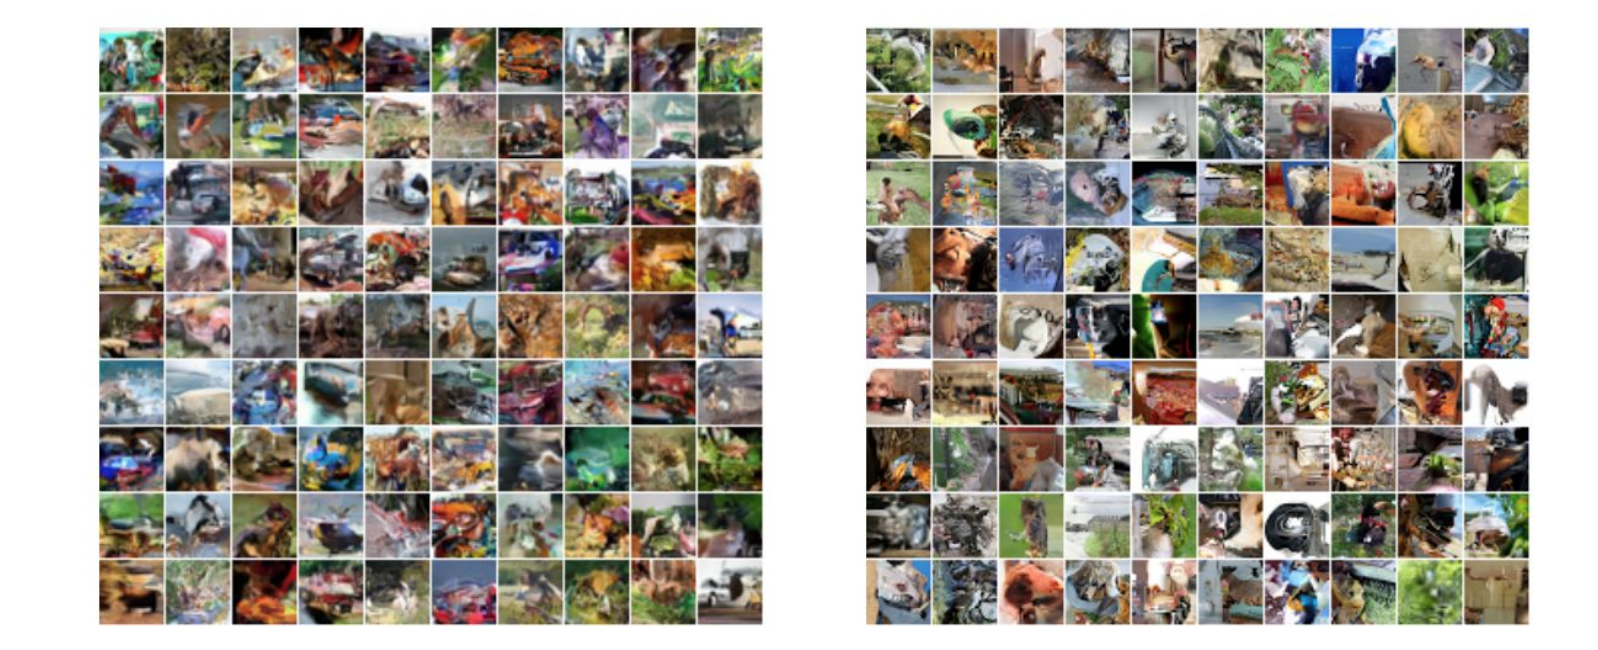
\includegraphics[width = .55\linewidth]{data/chapter-2/pixel_example.png} % 设定图片宽度相对于版心宽度,图片文件资源名
    \caption{pixel network 通过序列化的像素生成图像} % 图的题注
    \label{img:pix-example} % 与 autoref 关联,设定交叉引用和显示「图x.x」
\end{figure}




\section{数据库资源}

\subsection{艺术品交易数据库}

本文使用的数据库资源来自雅昌拍卖网艺术品交易数据库(auction.artron.net)。这是一个艺术品拍卖网站,数据库中关于艺术品以及艺术品交易的信息丰富,包括流通的艺术品的题目、图片、特征、作者、艺术品类别、交易价格、流通时间等等。我所用到的数据库中的信息包括两类如图~\ref{figure:数据库结构},一类是艺术品信息,另一类为艺术品相关的文章。

\begin{figure}[!htbp]
\centering
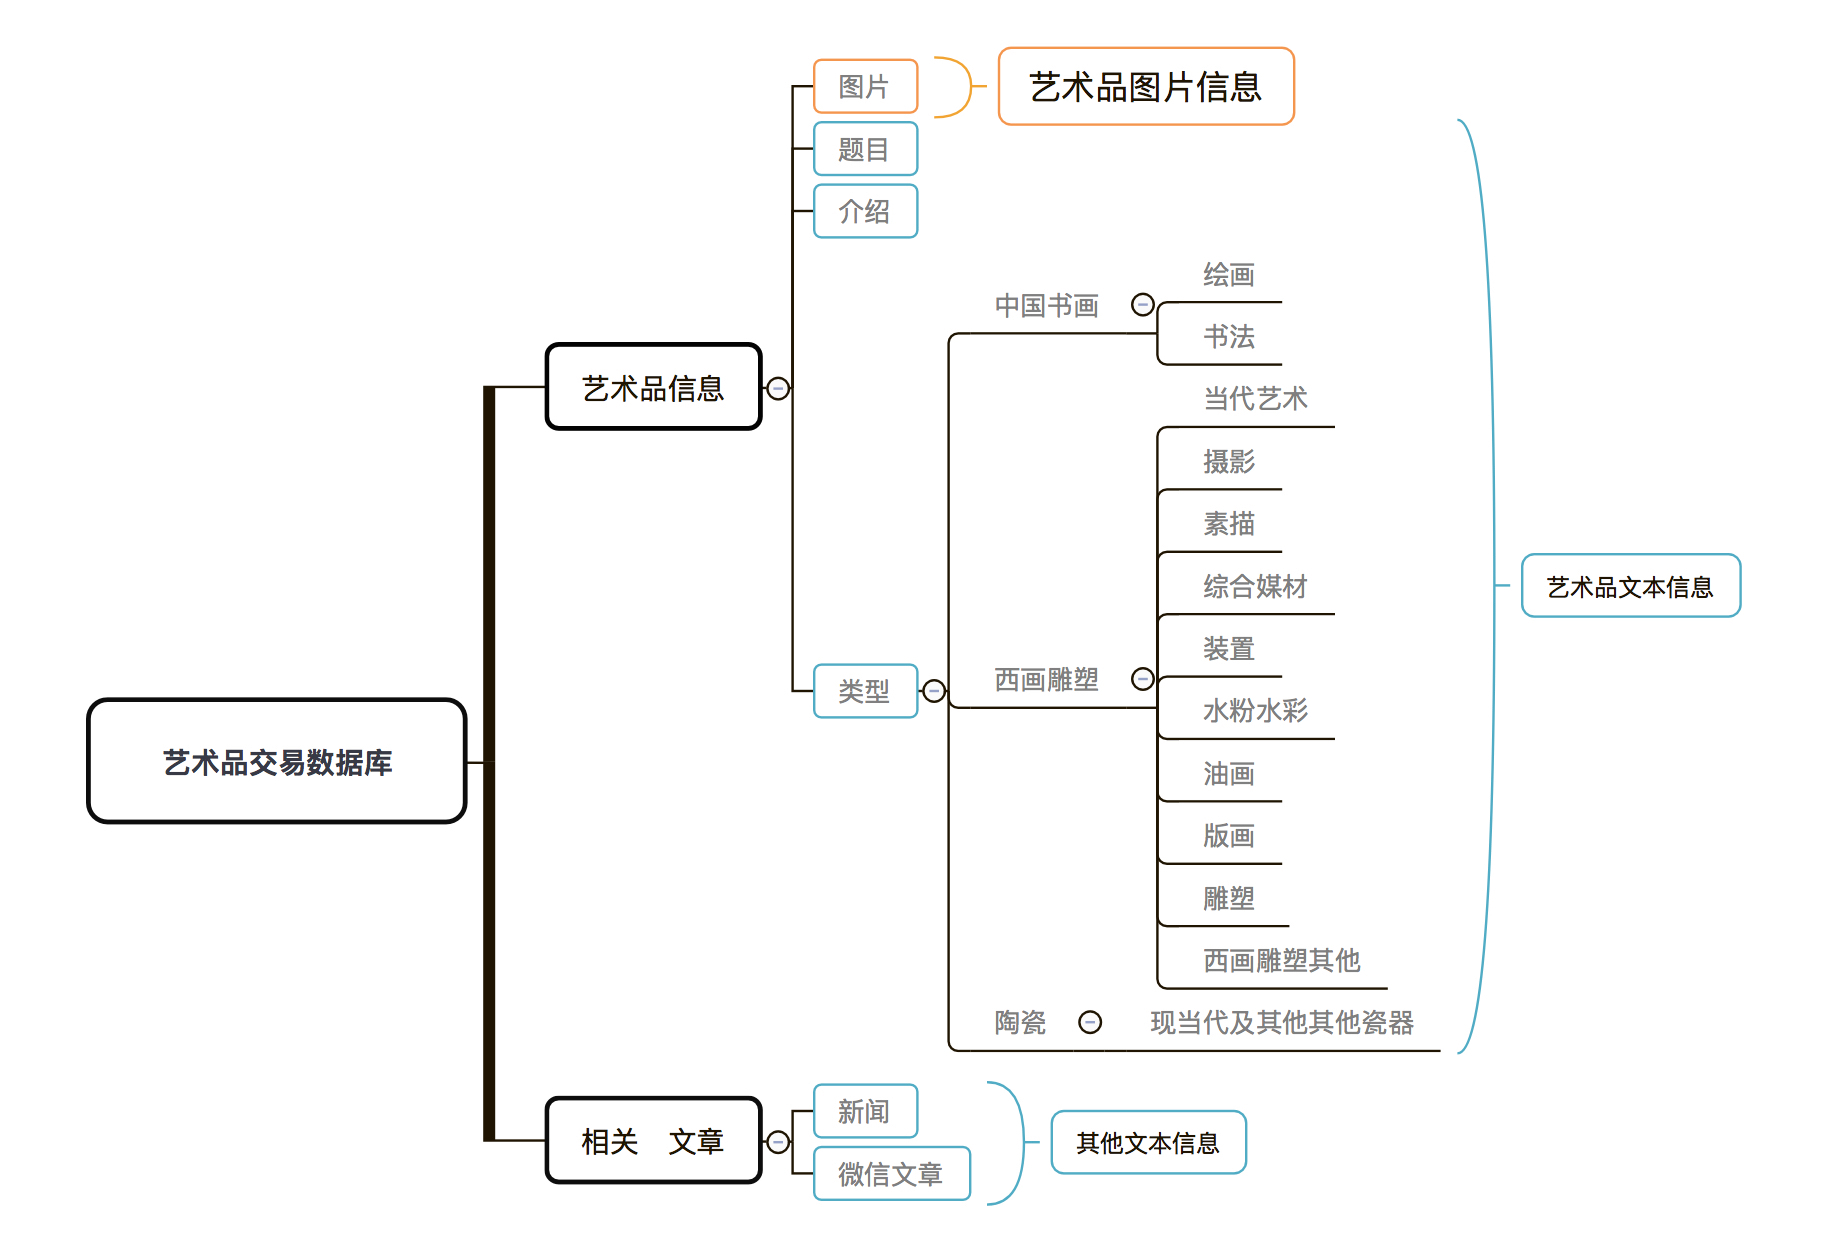
\includegraphics[width=\linewidth,keepaspectratio]{data/chapter-1/D02BCA18-F339-4988-9E23-E6C5E437BCCA.jpg}
\caption{数据库结构}
\label{figure:数据库结构}
\end{figure}

艺术品信息具体是指艺术品的题目、介绍,类型等文字描述(文本信息),以及艺术品的图片所在的url地址(可以下载到图像文件)。

每件艺术品都有对应的题目,艺术品的题目就是艺术品的名称,一般由艺术家命名,艺术品的名称和艺术品的内容常常是相匹配的。虽然也有一些情况艺术品的名称和内容表面上完全无关,但是艺术史上叫做“无题”的艺术品也何其之多,但是艺术品的题目作为艺术品的一部分,与艺术品的主题之间的关系紧密是无可辩驳的。

数据库中艺术品的类型分为中国书画、西画雕塑、陶瓷,在每个类型下再次细分。在中国书画下分为:绘画、书法。西画雕塑下分为:当代艺术、摄影、素描、综合媒材、装置、水粉水彩、油画、版画、雕塑、西画雕塑其它。陶瓷下分类为:现当代及其它瓷器。

数据库中艺术品的图片包括瓷器、雕塑等三维作品的照片和绘画、书法等二维作品的扫描件,由于数据库的数据缺失,极少量的艺术品并没有对应的艺术品的图片。

数据库中艺术品的介绍是艺术品交易时所附的艺术品介绍,内容包括并不限于对作者背景的介绍、该作品创作背景的介绍、作者风格的描述、作品风格和作品内容的描述等等,由于一些艺术品本身并没有对应的介绍文本以及数据库数据的缺失,一些艺术品没有对应的介绍文本。

艺术品相关的文章包括网站的新闻板块和网站微信公众号的文章,包括艺术品市场关注的新闻事件、热点、拍卖会宣传、艺术家专访、艺术相关杂文、艺术评论等各方面的文章。

\subsection{维基百科全文}
在涉及自然语言处理的语义搜索步骤中,我还使用了维基百科全文作为语料库,这一点将在下一章“语义编码的实现”一节中详细解释。


%\section{本章小结}



\chapter{基于语义识别的自动配色方案辅助设计工具}

\section{系统结构}

本系统的算法实现结构如图~\ref{figure:内部实现逻辑}

\begin{figure}[!htbp]
\centering
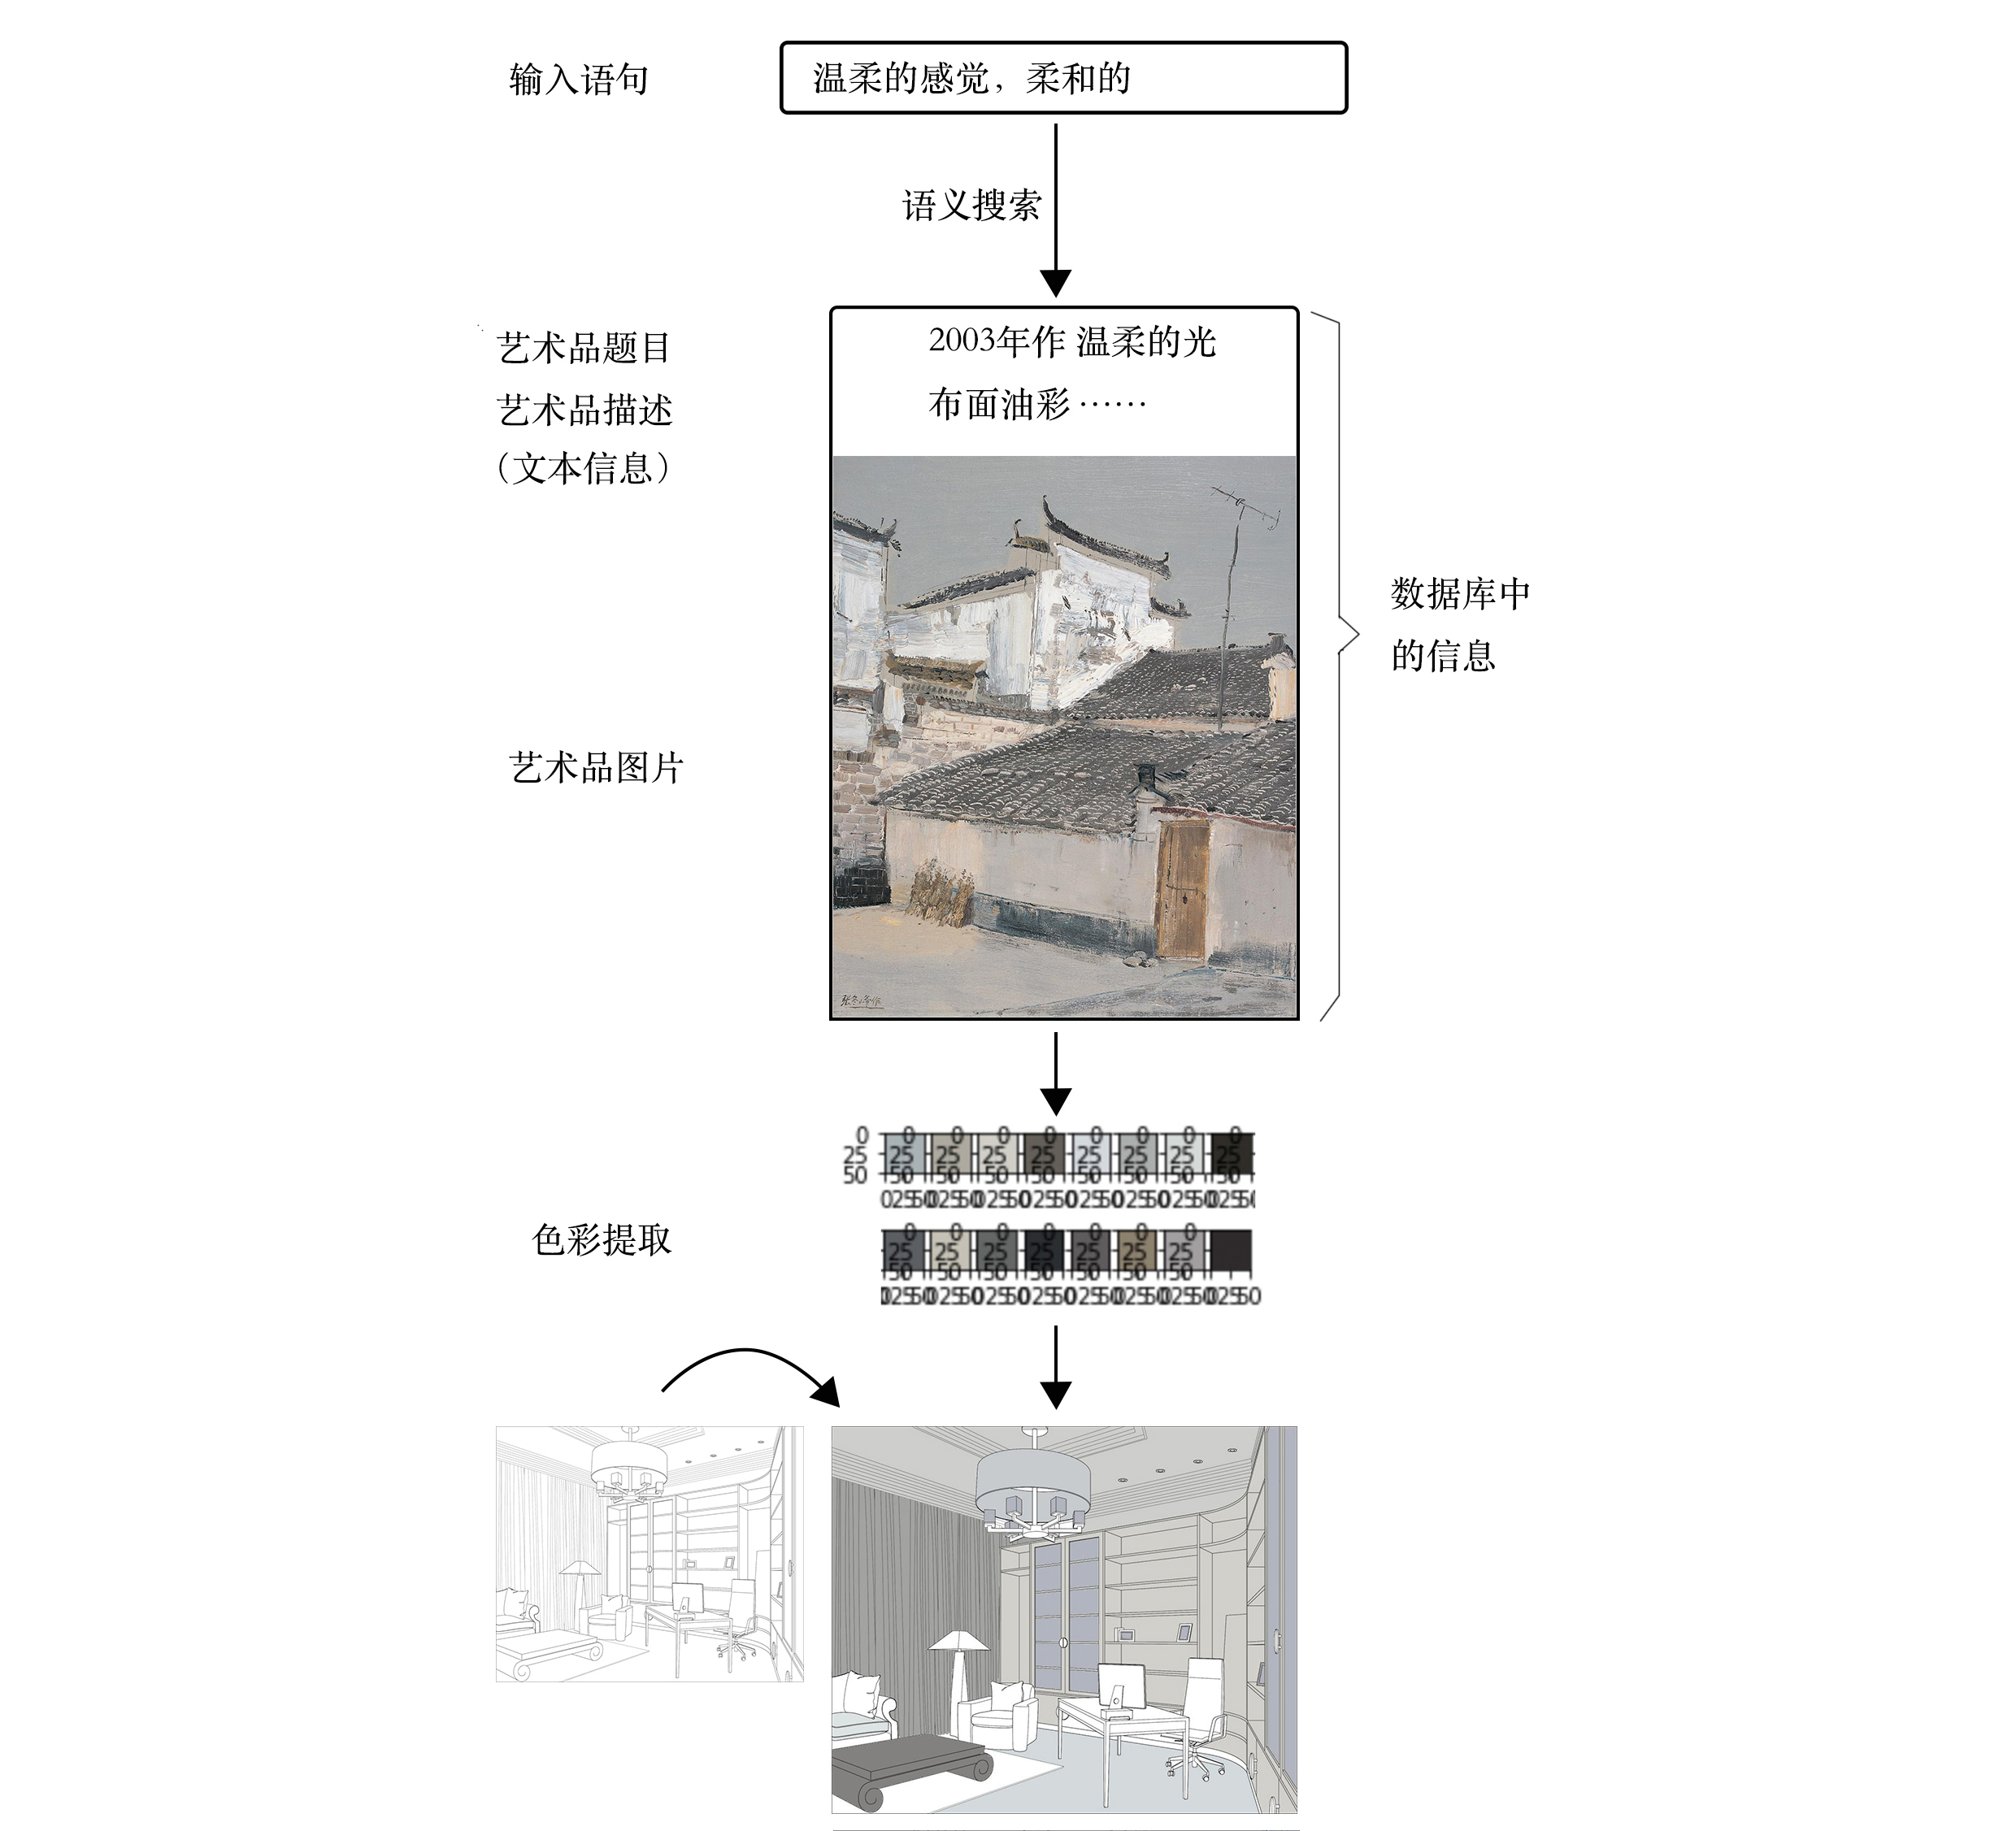
\includegraphics[width=\linewidth,keepaspectratio]{data/chapter-1/系统内部逻辑.jpg}
\caption{内部实现逻辑}
\label{figure:内部实现逻辑}
\end{figure}

本系统的整体思路为:首先,输入语句是对需求的文本描述,可以是词语,句子或不完整的句子。第二步,针对输入语句对艺术品的文本信息进行语义搜索,找出与之关联度高的艺术品文本信息。第三步,依据艺术品数据库中艺术品的图片信息和文本信息的隐藏信息关联匹配对应,即可以找出与输入文本关联度高的图片。之后,从图片中提取色彩方案,包括绘画作品的色彩和配色比例。最后,将提取的色彩方案运用到设计效果图上预览。

本系统的用户交互框架如图~\ref{figure:用户逻辑},对于用户来说,用户的使用逻辑是简单而清晰的,

\begin{figure}[!htbp]
\centering
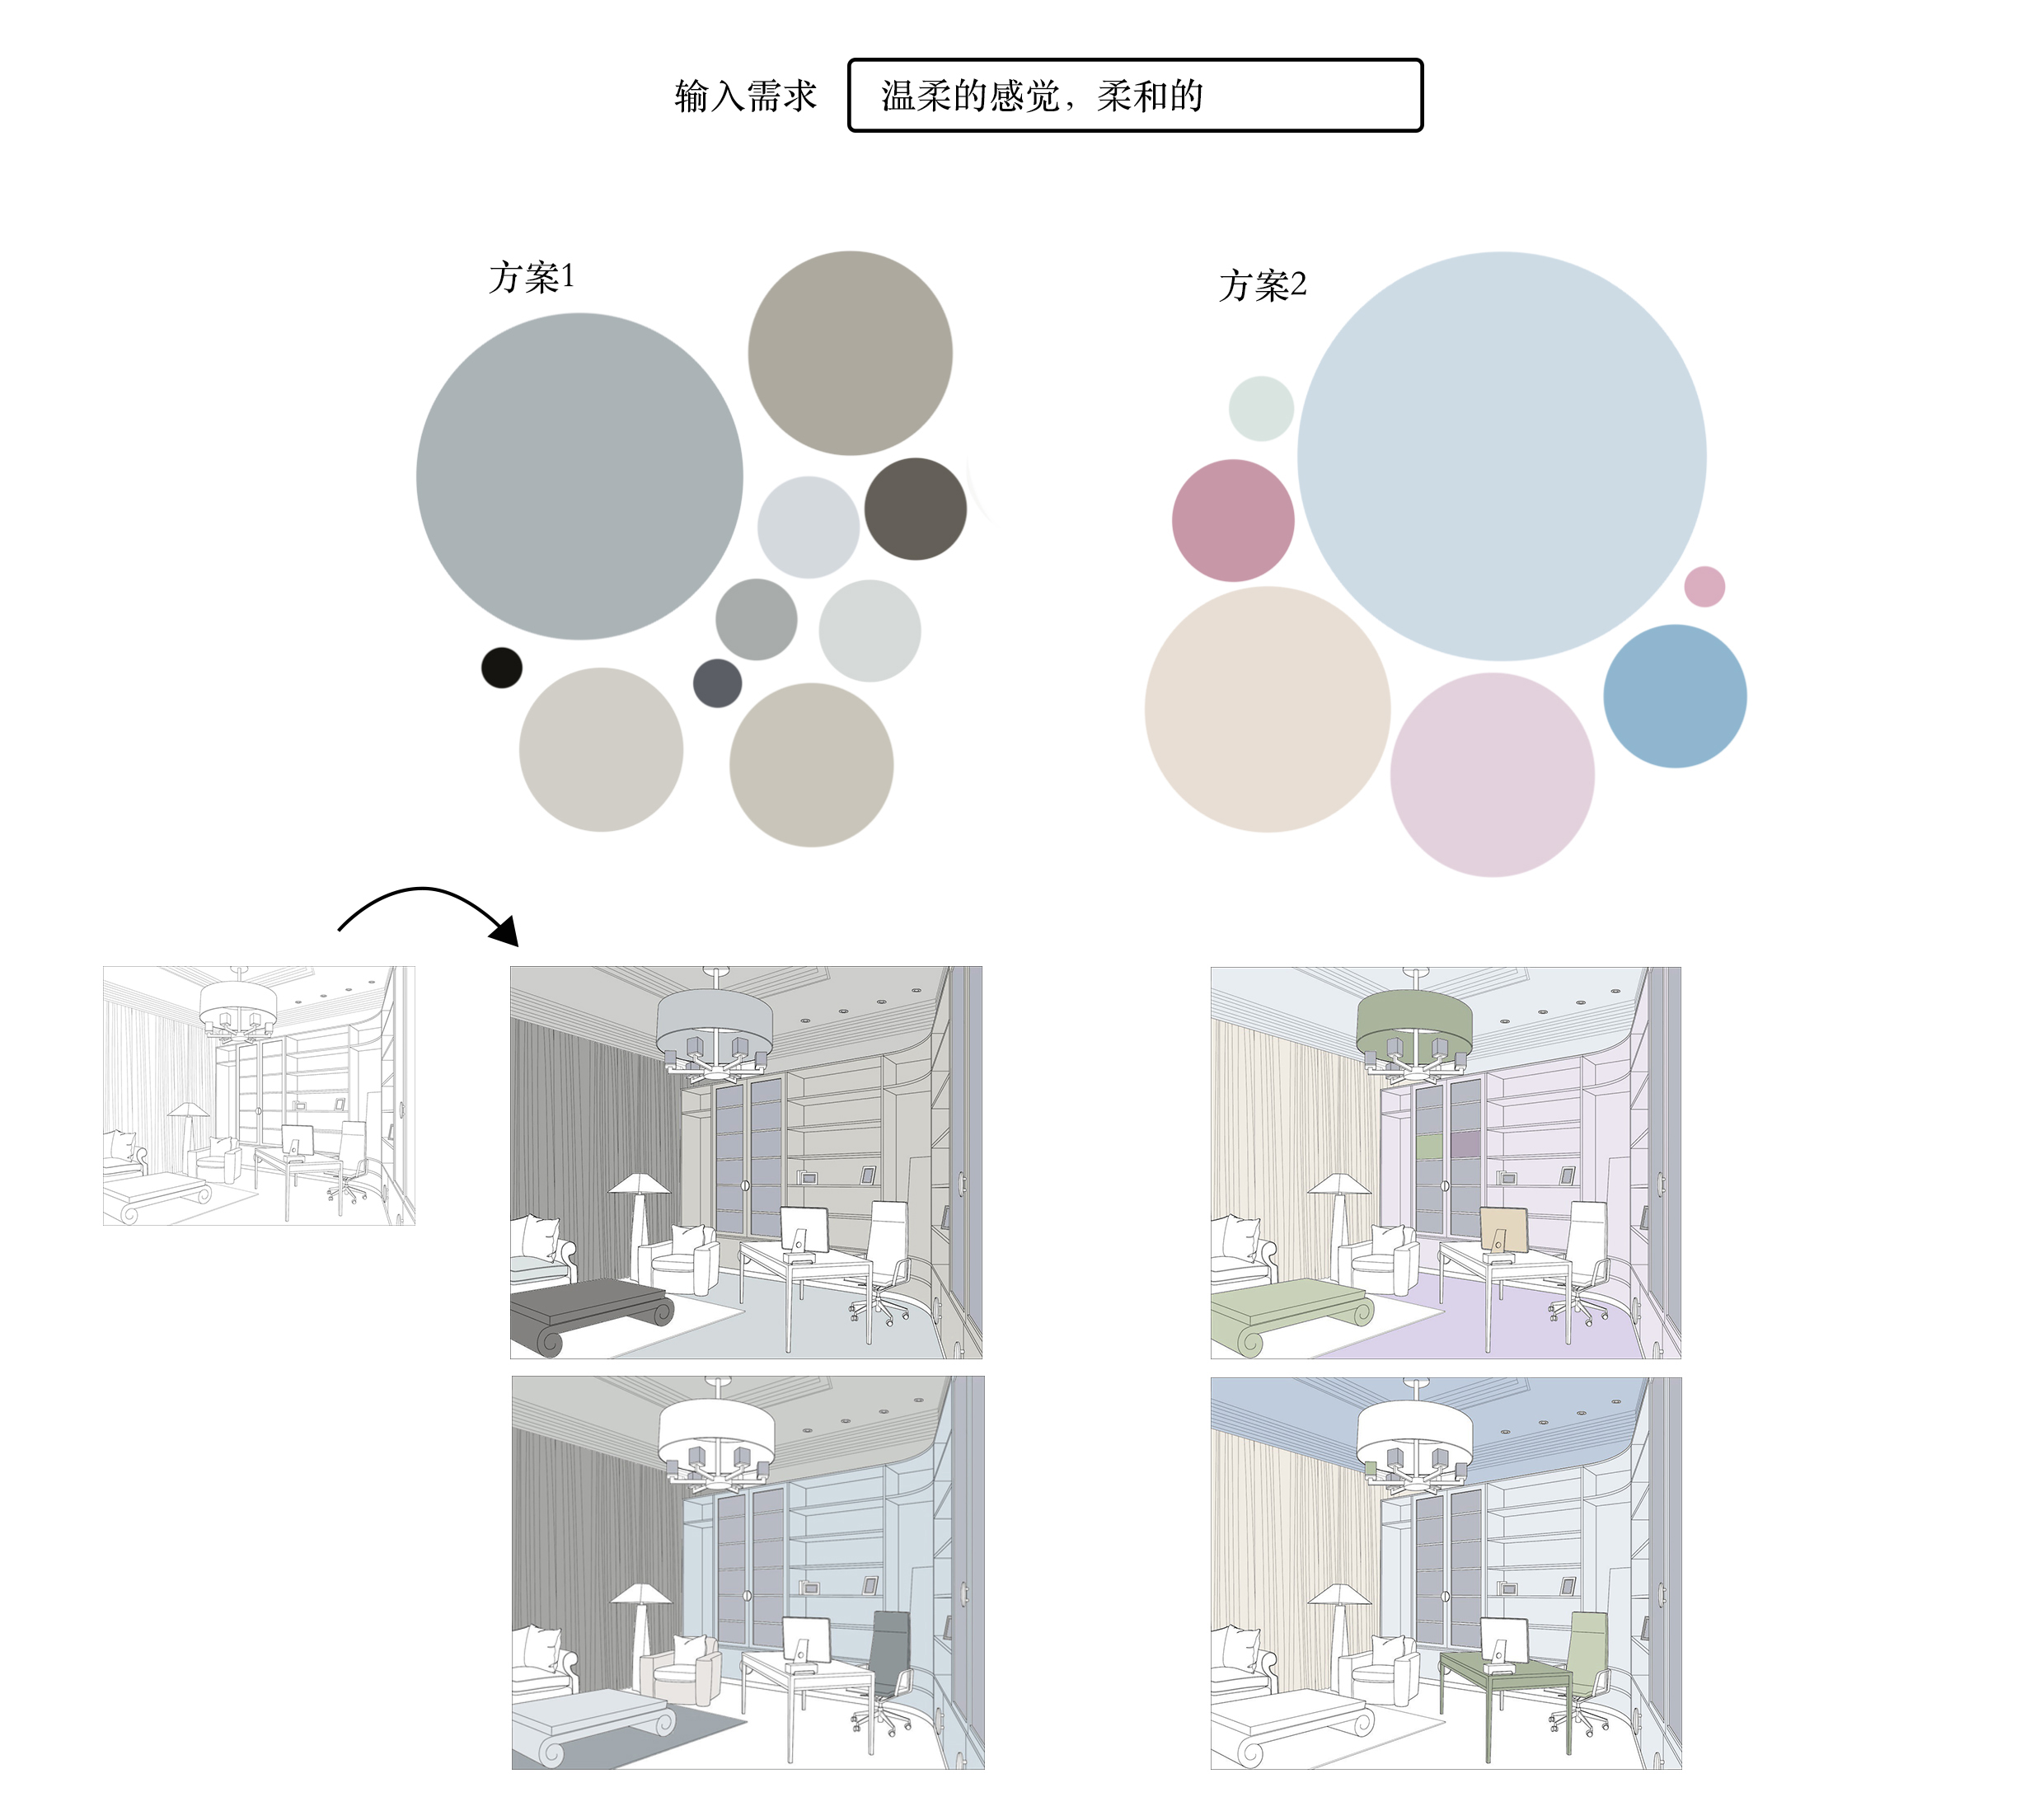
\includegraphics[width=\linewidth,keepaspectratio]{data/chapter-1/用户逻辑.jpg}
\caption{用户逻辑}
\label{figure:用户逻辑}
\end{figure}

搜索相匹配的艺术品这一步对用户来说是隐藏的,用户并不能看到相应的艺术品,而只得到色彩方案。这是为了让用户集中精力到他本来的任务中,关心配色方案而不用受到其他影响。输入设计需求的文本描述,就可以得到若干配色方案,并且可以每个配色方案都可以出现若干即时预览图,用户可以对各个配色方案有直接的感受。


\section{语义编码的实现}

\subsection{系统结构之语义搜索}

\begin{figure}[!htbp]
\centering
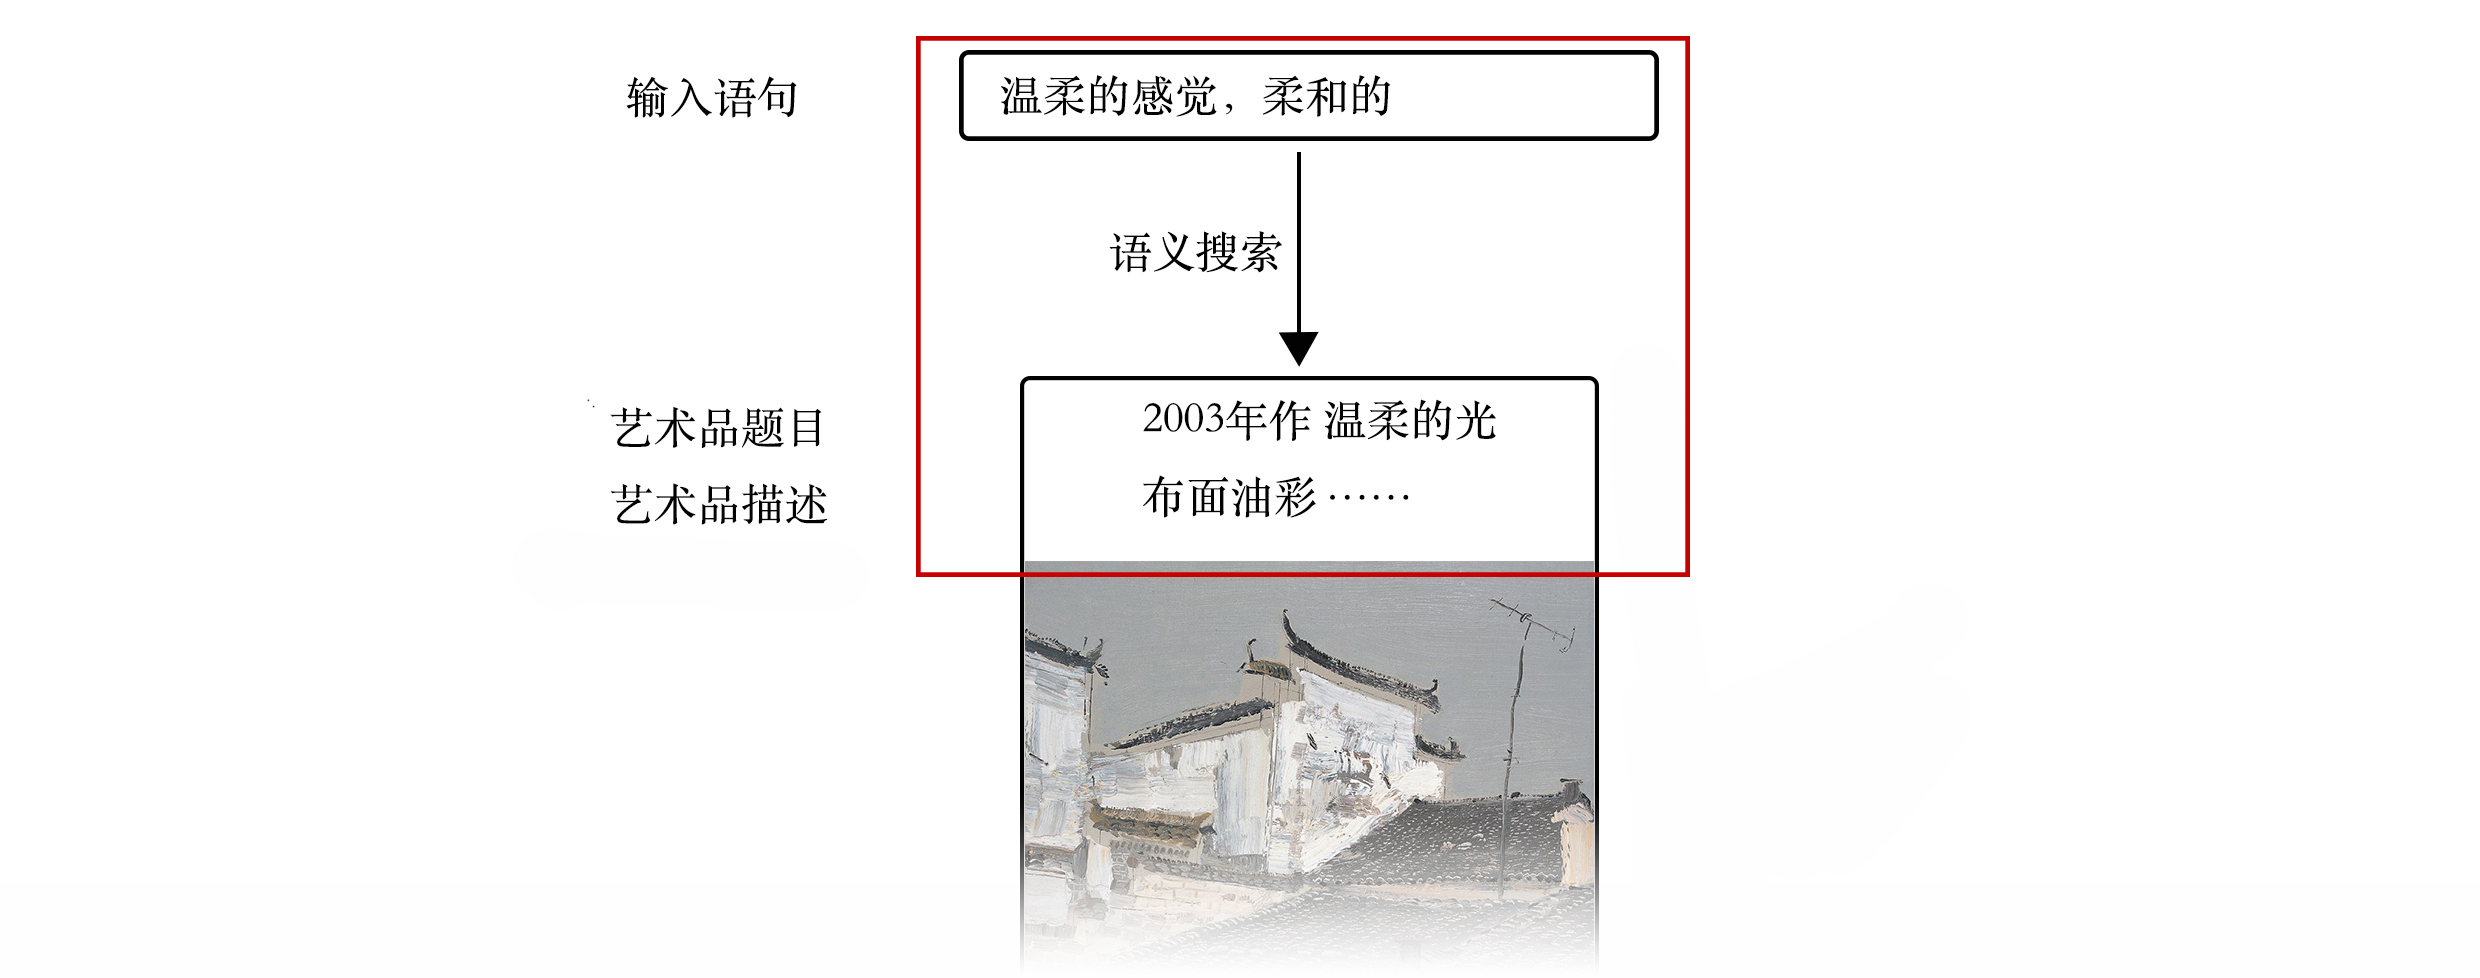
\includegraphics[width=\linewidth,keepaspectratio]{data/chapter-1/系统内部逻辑1步.jpg}
\caption{第一步:语义搜索}
\label{figure:语义搜索}
\end{figure}

图~\ref{figure:内部实现逻辑}中的第一步如上图~\ref{figure:语义搜索},就是搜索数据库中与用户输入相匹配的内容。要强调的是,我们的需求并非要提取关键词作为匹配,例如搜索含有某个词的字段,而是想做到搜索到词语意义相关的信息,例如输入“沮丧”可以匹配出“伤心,难过,忧伤的人”这样的字段,又例如输入“粉嫩”可以匹配出“少女”这样的字段。这就需要理解用户输入的内容和数据库中的文本内容,在其中作出意义上而非字面上的匹配。

\subsection{文本的向量化}

要使计算机理解文本的含义,从而进行搜索,对文本进行编码就需要满足以下三个要求:1.编码需要被计算机识别;2.编码需要包含单词的含义信息;3.所有的文本编码需要一定的整体同一性。

计算机理解文字的含义是困难的,即使计算机可以轻松的辨别出两句话是否一模一样,一句话中是否出现过某个单词,但是它却无法理解“苹果”和“梨”之间的关系(这对人类来说是常识),它也不能理解作为水果的“苹果”和“苹果”公司有什么不同(对于人类可以清楚的通过上下文理解这一点,不常混淆)。也就是说,文本的含义包括了语义,逻辑,上下文不同带来的多义。要用数字来表达这样复杂的信息,目前最好的解决方式是用向量来表达。

单词向量化是指将单词编码为向量形式,单词的向量化有多种方法,最简单的一种就是one-hot的向量。\cite{athier1997process}我们用一句话来举例子:“我 喜欢 吃 苹果,而 他 喜欢 吃 梨子。”这个句子长度为7个不同的单词。我们可以用这样的向量给每个单词编码,每个单词就可以表现为一个7维的向量,如表~\ref{table:one-hot},每个单词的向量为单词下的一列,就可以将一段文本的信息完整的保存进一个矩阵。

\begin{table}[!htbp]
\caption{one-hot向量}
\label{table:one-hot}
\centering
\begin{tabular}{|c|c|c|c|c|c|c|c|c|c|}
\hline
  & 我 & 喜欢 & 吃 & 苹果 & 而 & 他 & 喜欢 & 吃 & 梨子 \\
\hline
我 & 1 & 0 & 0 & 0 & 0 & 0 & 0 & 0 & 0 \\
\hline
喜欢 & 0 & 1 & 0 & 0 & 0 & 0 & 1 & 0 & 0 \\
\hline
吃 & 0 & 0 & 1 & 0 & 0 & 0 & 0 & 1 & 0 \\
\hline
… &  &  &  &  &  &  &  &  &  \\
\hline
\end{tabular}
\end{table}

这样的方法,如果对于文本长度较大的情况,就需要很大的空间储存这些向量,比如一本上万个单词的书籍,就需要单词的维度上万,里面大多数的位置又都是0。并且,这种方式对于不同文本来说并没有同一性,对于同一个词,不同的文本中必须有不同的词向量。最不好的一点是,这些词向量很难表示词的含义,例如近义词的向量和同类词语的向量,根本没有规律可循。

\begin{table}[!htbp]
\caption{词频向量}
\label{table:frequency-vec}
\centering
\begin{tabular}{|c|c|c|c|c|c|c|c|}
\hline
句子 & 我 & 喜欢 & 吃 & 苹果 & 而 & 他 & 梨子 \\
\hline
我喜欢吃苹果而他喜欢吃梨子 & 1 & 2 & 2 & 1 & 1 & 1 & 1 \\
\hline
我喜欢吃苹果,梨子 & 1 & 1 & 1 & 1 & 0 & 0 & 1 \\
\hline
他喜欢吃吃吃 & 0 & 1 & 3 & 0 & 0 & 1 & 0 \\
\hline
\end{tabular}
\end{table}

为了减少向量的维度,增加矩阵的密集程度,出现了基于词频的单词向量化。以我们的例句为例“喜欢”,“吃”这两个单词出现了两次,其他单词出现了一次。词频向量就是基于此构成。如表~\ref{table:frequency-vec},例如一篇文章中有表中的三句话,则每个单词的向量为单词下的一列,每句的向量为句子右侧的一行。词频向量和one-hot向量相比,维度有所下降,使用空间更有效率。词频也会记录一些文本的信息,不同的文本中单词的词频会有区别。然而完全从句子对单词计数,对词序信息完全忽略,同样难以提取文字本身的含义。

在此基础上的tf-idf的向量化不仅仅量化一个单词在一段文本中的频率,还考虑到在所有文本中单词出现的情况,这样就可以表征出一个单词和某段文本的关系。\cite{xia2011improvement}$tfidf = tf(t,d)*idf(t,D)$,其中 $tf(t,d)$ (term frequency)表征单词t出现在文本d中的频率。它可以有多种形式,比如$tf(t,d)=f_td$,$f_td$表示单词t出现在文本d中次数;或者考虑到文本到长度$tf(t,d)= \frac{f_td}{n_{in document}}$,$n_{in document}$指文章总共的单词数,$tf(t,d)$即出现在文本中的频率;甚至也可以是布尔的,当文本d中出现词t则 $tf(t,d)=1$ 否则$tf(t,d)=0$,等等。idf(inverse document frequency)定义为$idf(t,D) = log\frac{N}{n_{t occurs}}$ ,$N$表示总的文档数,$n_{t occurs}$表示含有单词t的文档数。

以之前的三句话为例:(a)我 喜欢 吃 苹果 而 他 喜欢 吃 梨子。(b)我 喜欢 吃 苹果。(c)我 喜欢 吃 吃 吃。则对于单词“我”,有:$tf(“I”,a)= \frac{1}{9}$,$tf(“I”,b)= \frac{1}{4}$,那么句子b中“我”这个词占整体比例更高。但对于所有文本,$idf(“I”,D) = log\frac{3}{3} = 0$,每个句子都出现了“我”这个词,所以$tfidf(“I”,a) = tfidf(“I”,b) = 0$。处理文档大量时,对于一些非常常见的词,比如“那个”“这个”这样的词,可以认为它们没什么意义,就会出现这种情况。而比如对于单词“苹果”,$tf(“apple”,a)= \frac{1}{9}$,$tf(“apple”,b)= \frac{1}{4}$,$idf(“apple”,D) = log\frac{3}{2} $,就会出现$tfidf(“apple”,a) = 0.045$,$tfidf(“apple”,b) = 0.1$。我以这三个句子计算了单词“我”和单词“苹果”的向量如表~\ref{table:tfidf-vec}:

\begin{table}[!htbp]
\caption{tfidf向量}
\label{table:tfidf-vec}
\centering
\begin{tabular}{|c|c|c|c|}
\hline
句子 & 我喜欢吃苹果而他喜欢吃梨子 & 我喜欢吃苹果 & 我喜欢吃吃吃  \\
\hline
我 & 0 & 0 & 0  \\
\hline
苹果 & 0.045 & 0.1 & 0 \\
\hline
… &  &  &  \\
\hline
\end{tabular}
\end{table}

只要有足够量的文本,tf-idf向量可以在文本间做比较,然而还有一个问题没有解决,那就是它仍然不包含单词语义的信息。在构建tf-idf向量的过程中,只用到了文本中单词的数量,完全没有使用单词的顺序信息,而文本中单词顺序所含有的信息是很重要的,如何将这些信息提取出来呢。

如果我们考虑上下文构建向量。对于句子“我 喜欢 吃 苹果 而 他 喜欢 吃 梨子”。将每个词前后对它有影响的单词数量,称为上下文窗口大小(context window)。比如,对于单词“喜欢”,在窗口大小为3时,单词“吃”在它周围出现的次数共2次,“我”、“苹果”、“他”、“梨子”、“而”各一次。如表~\ref{table:context}:

\begin{table}[!htbp]
\caption{上下文向量}
\label{table:context}
\centering
\begin{tabular}{|c|c|c|c|c|c|c|c|}
\hline
句子 & 我 & 喜欢 & 吃 & 苹果 & 而 & 他 & 梨子 \\
\hline
我   & 0 & 1 & 1 & 1 & 0 & 0 & 0 \\
\hline
喜欢 & 1 & 0 & 2 & 2 & 2 & 1 & 1 \\
\hline
吃   & 1 & 2 & 0 & 1 & 2 & 2 & 1 \\
\hline
苹果 & 1 & 2 & 1 & 0 & 1 & 1 & 0 \\
\hline
而   & 0 & 2 & 2 & 1 & 0 & 1 & 1 \\
\hline
他   & 0 & 1 & 2 & 1 & 1 & 0 & 1 \\
\hline
梨子 & 0 & 1 & 1 & 0 & 1 & 1 & 0 \\
\hline
\end{tabular}
\end{table}

在此基础上,如果我们采用一点统计学和数学的知识,使用神经网络的算法,就可以从文本中提取出更多的信息。word2vect就是这样一种算法,虽然前面所述都是单词向量化都方法,但word2vect被 Mitolov 等引入到自然语言领域之后,向量前所未有的拥有了密集的信息。对于一个出现在文本中的单词,在知道周围的词语的情况下,就能够预测出这个单词是某个单词的可能性。\cite{baroni2014don}比如“我喜欢吃(a)”,a是单词“苹果”的可能性就比a是单词“因为”的可能性更高。在非常大量文本的情况下,“苹果”和“梨子”常常出现在相似的环境下,算法就将计算得到它们的向量是相似的,从而被归为相似的词语。\cite{DBLP:journals/corr/abs-1301-3781}

word2vect由CBOW(Continuous bag of words) 和 Skip-gram model 两个部分共同组成。\cite{DBLP:journals/corr/abs-1708-00107}CBOW的工作方式为以全文训练神经网络,以求输入神经网络一个单词,输出他周围的一个单词。以one-hot向量编码的句子“我 喜欢 吃 苹果 而 他 喜欢 吃 梨子”作为例子,则全文的矩阵如表~\ref{table:one-hot},对于其中“喜欢”这个单词,则具体为假如输入“喜欢”的向量,则期望输出“吃”的向量。\cite{Mikolov:2013:DRW:2999792.2999959}

\begin{table}[!htbp]
\caption{输入}
\label{table:cbow-input}
\centering
\begin{tabular}{|c|c|c|c|c|c|c|c|c|c|}
\hline
喜欢 & 0 & 1 & 0 & 0 & 0 & 0 & 1 & 0 & 0 \\
\hline
\end{tabular}
\end{table}

\begin{table}[!htbp]
\caption{输出}
\label{table:cbow-output}
\centering
\begin{tabular}{|c|c|c|c|c|c|c|c|c|c|}
\hline
吃 & 0 & 0 & 1 & 0 & 0 & 0 & 0 & 1 & 0 \\
\hline
\end{tabular}
\end{table}

CBOW算法结构如图~\ref{figure:CBOW网络结构},假如输入“喜欢”的向量 $(0,1,0,0,0,0,0)$,则期望输出“吃”的向量$(0,0,1,0,0,0,0)$。输入为${1}\times{V}$的矩阵(在这里V为7),隐藏—输入层为${V}\times{N}$的矩阵,隐藏—输出层为${N}\times{V}$。N就是我们选择的最终得到的词向量的维度。输入为${V}\times{1}$的矩阵,这个矩阵的每个位置对应的是one-hot编码中该位置单词出现的概率。在层与层之间没有激活函数,而是线性函数。使用计算出的输出值和期望的输出值之间的误差作为loss函数,反向传播适应得到维度为N的权重$\vec{W}$。与此同时,单词"吃"对应的输入还有“苹果”或“梨”,或者在窗口大小更大时的其他单词。多个权重平均的向量就是单词“吃”的向量。

\begin{figure}[!htbp]
\centering
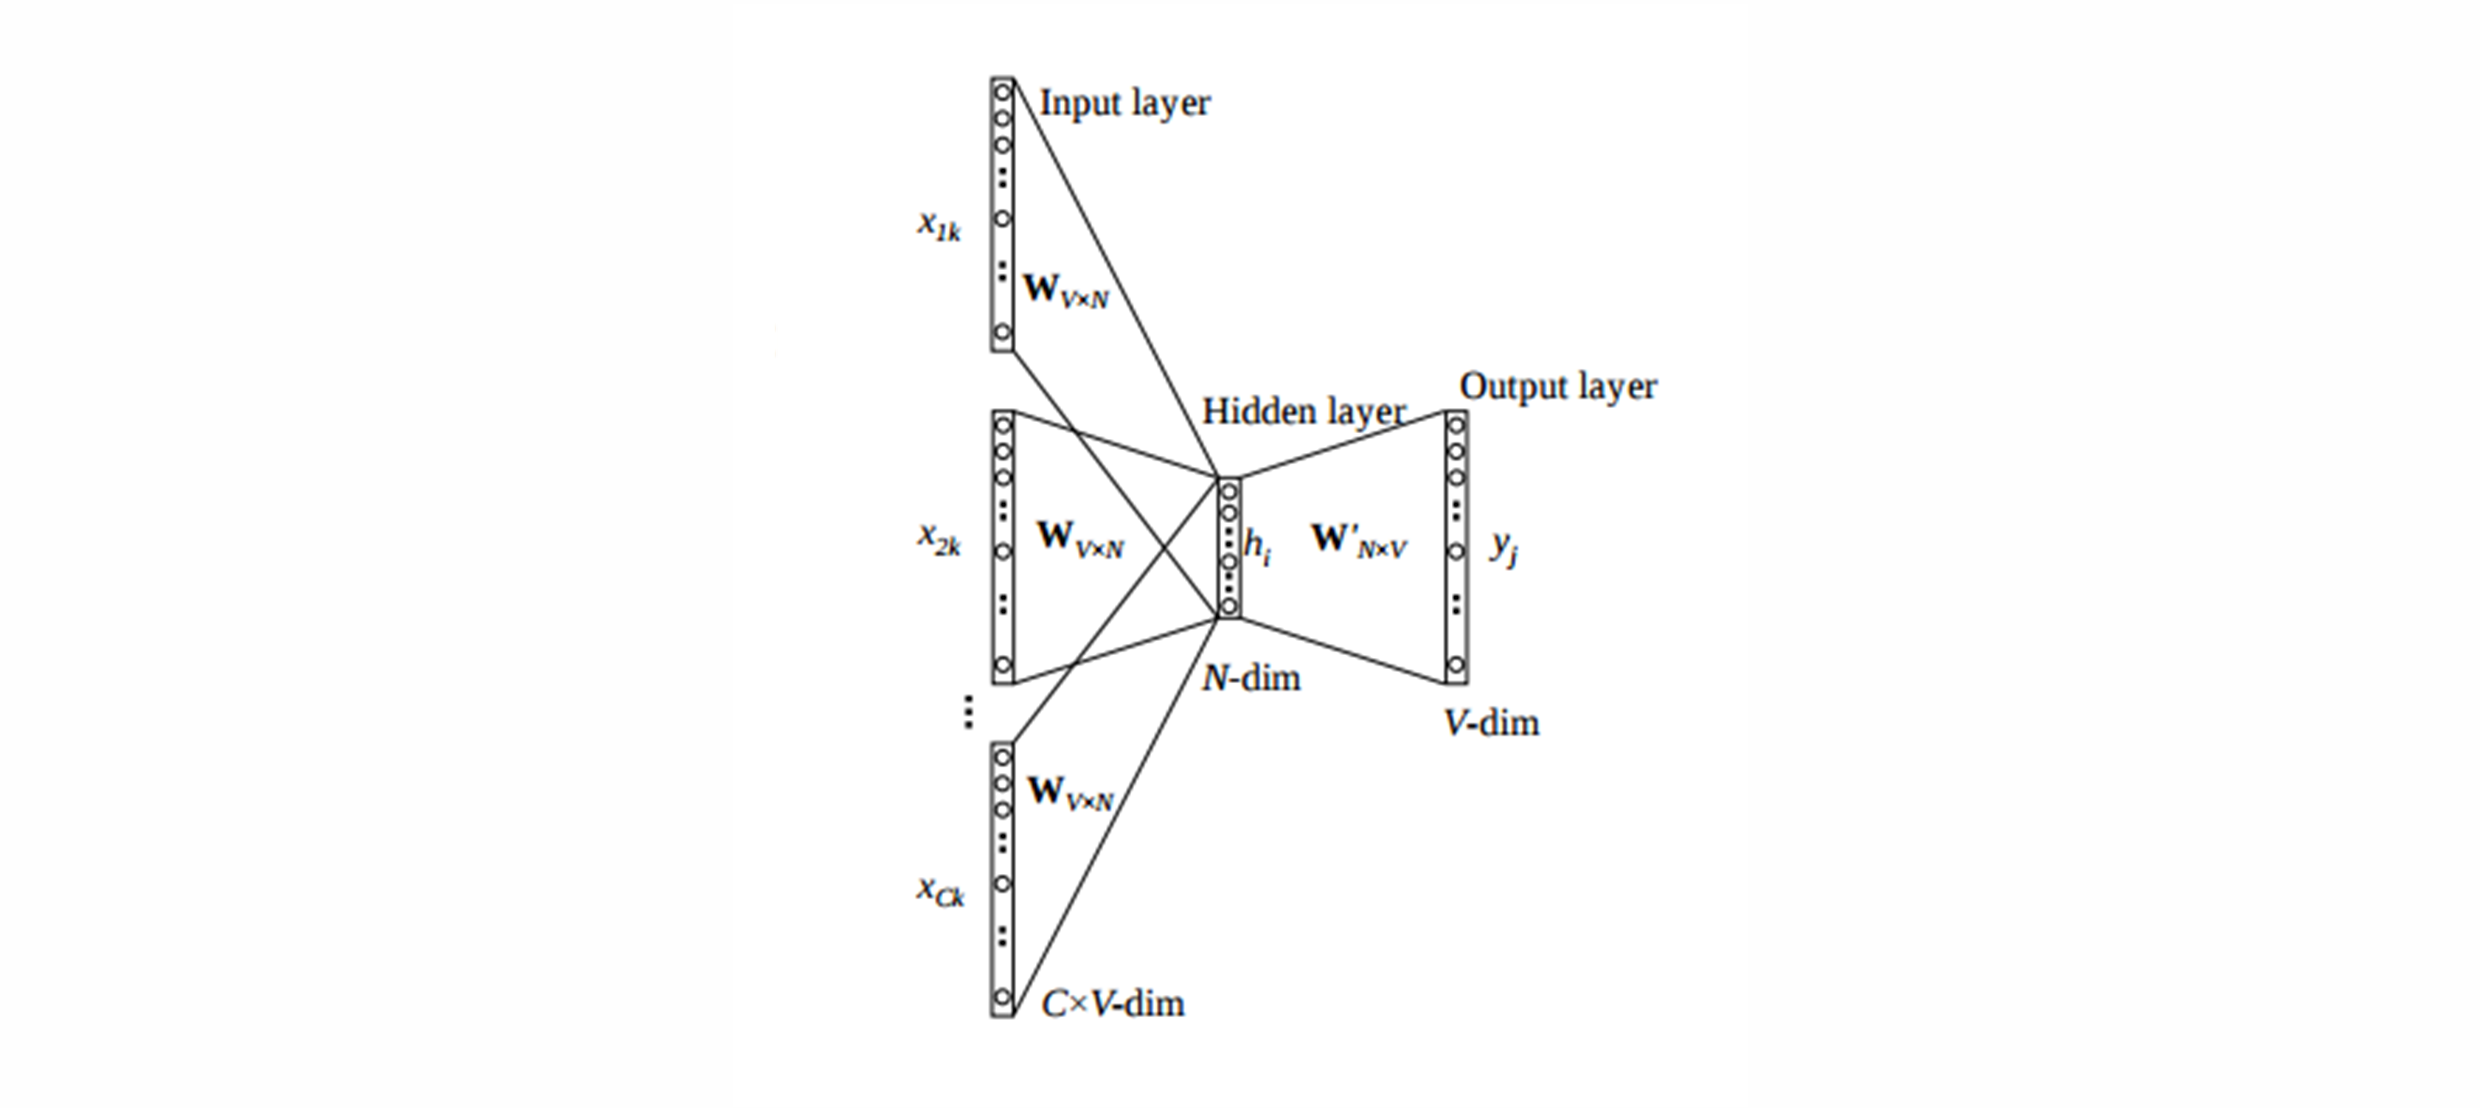
\includegraphics[width=\linewidth,keepaspectratio]{data/chapter-1/Screenshot-from-2017-06-04-22-05-44.png}
\caption{CBOW model}
\label{figure:CBOW网络结构}
\end{figure}

而Skip-gram model与之相似,只是输入的单词“喜欢”对应的输出有“我”,“他”,或者在窗口大小更大时的其他单词。对于多个输出单词就有多个误差向量,多个误差向量构成总的误差向量,反向传播适应得到维度为N的权重$\vec{W}$,即为单词“喜欢”的向量。

\begin{figure}[!htbp]
\centering
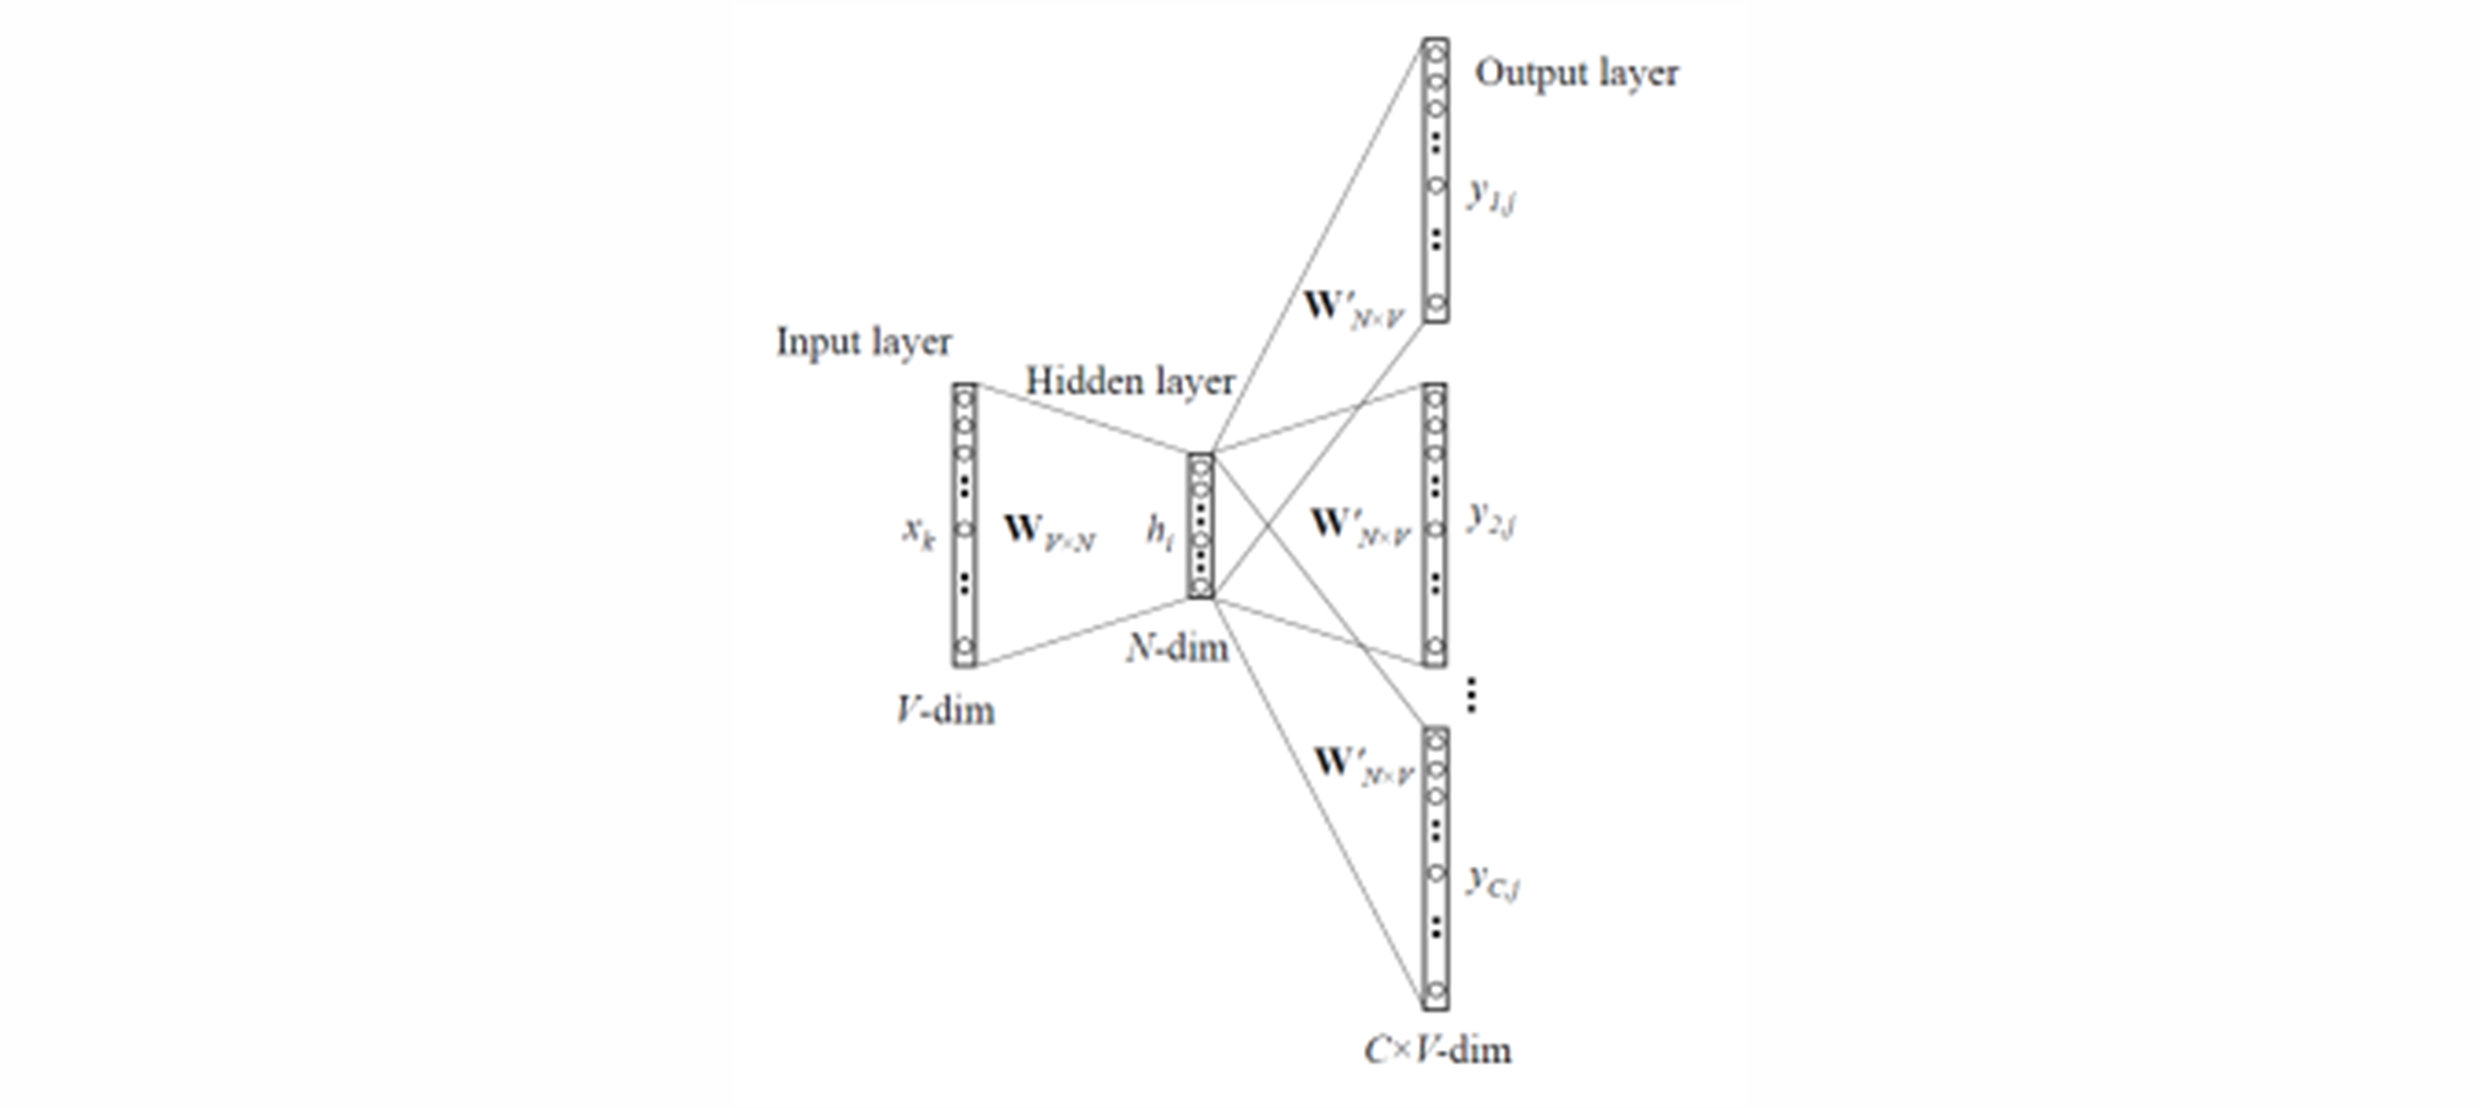
\includegraphics[width=\linewidth,keepaspectratio]{data/chapter-1/Capture2-276x300.png}
\caption{Skip-gram model}
\label{figure:Skip-gram网络结构}
\end{figure}

这种充分采用文字顺序的算法拥有很多很好的特性。比如,向量距离接近的单词意义也接近。更神奇的是,在训练文本多且全面的情况下,代表“女人”的向量和代表“妈妈”的向量之间的距离,与代表“男人”的向量和代表“爸爸”的向量之间的距离相等,即“女人”-“妈妈”=“男人”-“爸爸”;“苹果”这个单词的向量,同时和“梨子”的向量以及“IBM”的向量距离相等;由于是从文字的顺序提取信息,所以对于各种语言该模型都适用,也说明了提取的信息是语义上的而不仅仅是文本上的。

\subsection{本系统的单词向量化}

在介绍本系统的单词向量化之前,先要介绍我所使用的训练数据,训练词向量的数据来自两个来源,1.维基百科全文;2.艺术品交易数据库中的文本信息。其中艺术品交易数据库中的文本信息包含以下几种:1.艺术品交易数据库中每个艺术品的文本信息(包括艺术品的题目、描述和介绍、类型等);2.艺术品交易数据库中的所有文章(包括艺术品相关的新闻报道、微信文章、评论文章、艺术家专访等相关文章)。艺术品交易数据库中的文本信息是对艺术这一话题的加强训练。而采用维基百科的原因是,如果没有维基百科数据库,则当输入艺术品数据库中不存在的日常用语时就无法理解。为了系统能够响应人自然场景下的语言,采用一个普适的文本数据是非常必要的。对文本进行繁简体转化、中文分词之后,就可以作为训练使用的文本。

这样的庞大数据带来了更好的文本语义理解,但是也带来了计算量的问题。使用CBOW模型对单词进行word2vec向量化的过程中,如果文本有10000个单词,那么隐藏—输入层和隐藏—输出层就会是 ${10000}\times{N}$和${N}\times{10000}$的矩阵,需要反向传播调整和适应其中的每个权重计算量将会非常大,而维基百科和艺术品交易数据库带来的词量更是远大于此,对于如此大的计算量需要采用哈夫曼树进行优化,从而可以利用Hierarchical Softmax加速。\cite{DBLP:journals/corr/abs-1801-09797}

\begin{figure}[!htbp]
\centering
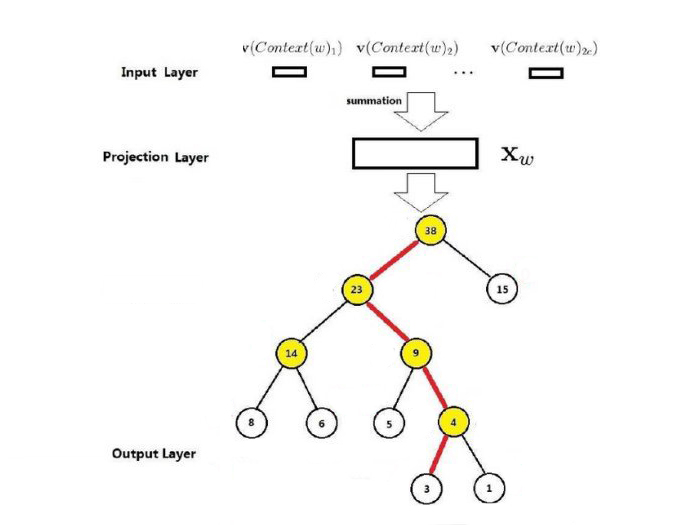
\includegraphics[width=\linewidth,keepaspectratio]{data/chapter-1/006iXRQMzy75IEZuWeoc4&690}
\caption{使用哈夫曼树的CBOW model}
\label{figure:使用哈夫曼树的CBOW model}
\end{figure}

哈夫曼树(Huffman Tree)又叫最优二叉树,是给定n个权值作为n个叶子结点,构造一棵二叉树,使得带权路径长度达到最小。哈夫曼树是带权路径长度最短的树,权值越大的结点离根越近。Skip-gram model的输出层使用哈夫曼树,总的文本中的每个词对应哈夫曼树中的一个叶子节点 (每个节点对应一个最后得到的word2vec词向量),每个非叶子节点定义一个向量(起到辅助的作用)。对于词典中的任意单词,哈夫曼树中必然存在唯一一条从根节点到该单词对应的路径,这样对于每一个单词,输出层只需要调整哈夫曼树路径上的向量。如果对于有V个单词的文本来说,本来隐藏—输入层和隐藏—输出层需要反向传播调整 ${V}\times{N}$和${N}\times{V}$个值,现在在哈夫曼树上每次二分产生一个概率,只需要经过log(V)次运算就得到了单词a出现的概率$p(a|context(a))$。

与此同时,本系统的word2vec还使用了以下的策略,把常见的词组作为一个新的单词增加到词典中,比如“苹果手机”;少采样常见的词,比如“而”“就”这些出现频率非常高的词其实它的表达的意思很少;采用Negative Sampling策略,通过负采样,每次修改其中一小部分weight,而不是全部。这些策略减少了训练的计算量,而且提升了最后word vector的质量。\cite{mikolov2013distributed}\cite{DBLP:journals/corr/abs-1301-3781}\cite{DBLP:journals/corr/abs-1801-10198}

CBOW模型实际上只考虑了单词有哪些上下文,而并未考虑单词的顺序,比如“我喜欢苹果”和“苹果喜欢我”在CBOW模型中的特征是一样的。加入了 N-gram 特征将“我-喜欢”和“喜欢-我”也加入单词的特征,也使用n-gram特征来将局部词序考虑在内,比如“女-朋友”“陶-瓷”。可以得到表达意义更准确的词向量。

使用上述的文本和模型训练维度为300的词向量,词典中包含全部文本中出现的单词。使用此词典构成输入语句和艺术品信息的语句向量。


\subsection{本系统的句向量建模}

在本系统中,需要语义搜索的内容并不是单词。输入语句是使用者输入的,不确定的语句,可能是一个或数个词语、短语、完整的或不完整的句子,总的说来,是一个或多个单词的序列,之后我们将其称为“输入语句”,即和我们平时口语采用的语言是相似的,不拘结构但求表达需求。而数据库中每个艺术品的文本信息由艺术品的题目、介绍,类型三个部分组成,短至一个词语(在文本信息只有一个单词的题目的时候),长至数段话(在文本信息包括大量描述和介绍的时候),总的来说也是一个或多个单词的序列,之后我们将其称为“艺术品语句”。需要从使用者输入的语句定位到某一件艺术品,那么就需要输入语句的含义,和某件艺术品语句的含义相匹配。

要提取一段语言的意义,就需要将这多个表达单词意义的向量转化为一个转化语句意思的向量。在这个将多个词向量加和为语句向量的过程,需要考虑这三点:

1.词汇的含义,语句由词汇构成,语句中词汇的意思对语句的含义是决定性的,比如一张油画的名字叫做“忧伤的河流”说的就是忧伤,不是喜悦,是河流,不是山川。

2.词汇的频率,在语句中词汇出现的频率会对语句的意义产生影响,这样的影响并非线性的,有时,频率高的词表达的含义反而少,比如“作者非常非常思念家乡”,中出现了两个“非常”,表达比“非常”更深的程度,但是句子主要要表达的意思仍然是“作者思念家乡”,这句话和“作者很思念家乡”的含义相似,而和“我非常非常喜欢吃苹果”是不同的;而有的时候频率高的单词直接是这段文本中的重要主题和中心。大概率的,总体文本中频率高的词带来的含义有限,这些词比如“有”“这”“那”,并不影响语句的意义,而总体文本中概率一般然而特定文本中频率高的词,比如在某个作品的描述中常常出现“热烈”“欢快”,往往对这一文本的语义的影响很大。

3.词汇的位置。词汇的位置有时也代表了词汇含义的重要性。语言是结构性的序列,在结构的某一位置上的词语往往代表更重要的含义。对于词语构成语句的过程,这个位置的重要性很灵活。比如对于语句“作者非常思念家乡”,如果这句话处在一个环境中,上一句话是“谁思念家乡了?”,那么最重要的位置就是主语的“作者”,而如果上一句话是“作者思念什么”,那么最重要的位置就是宾语“家乡”。另外,如果考虑句子构成完整段落的过程,段落的第一句话和最后一句话,由于可能是总起和总结的句子,所以格外重要,这也是考察位置得到的信息。

对单词向量直接加和求得输入语句的向量是最简单的方法,即$\vec{S}=\sum_{i=0}^{n}{w_i}$。其中$\vec{S}$指据向量,句子中有n个单词,${w_i}$指第i个单词的词向量。\cite{DBLP:journals/corr/abs-1801-10198}这种方法简单快捷,但是它只考虑了语句中词汇的含义,并没有考虑到词汇的频率和词汇的位置对句向量的影响。会导致语句中重复出现的词语对语句影响严重的情况,另外也会让一些本来并不代表意义的单词占比较大,比如对于语句“我要一个柔和一点的色彩方案”,这句话中“柔和”其实是最关注的一个词,但是由于干扰信息太多,如果直接加和,这句话的向量会和“我要一个欢快一点的色彩方案”更近,而与单词“柔和”并不相近。更突出的一个例子是,很多作品的题目中会出现作品的媒介比如“儿童 布面油画”,“温柔的风 油画”等等,其中,单词“布面”、”油画“等,它们在整体文本中大量出现,但对于每个作品已经有了明确的分类信息,文本信息中更多的是为了匹配作品的内容和色彩风格,它们就并非与作品色彩风格有关的单词。

在这种情况下,我采用了加权加和的方法,即$ \vec{S} =\sum_{i=0}^{n}{ \vec{w_i}}*{weight(w_i)}$ ,这样可以通过权重过滤掉干扰信息。\cite{DBLP:journals/corr/abs-1708-00107}\cite{DBLP:journals/corr/abs-1801-10198}我使用单词在总体文本中的词频作为权重分析的来源,在总体文本中出现频率越高的词就说明它是不重要的(如果一个单词出现在每一句话中,那么这个单词当对分辨每句话的意义并没有价值)。如此,则权重$ weight(w_i)=\frac{1}{frequency(w_i)}$ ,句向量的计算方式则为:

$$ \vec{S} =normalization(\sum_{i=0}^{n}{ \frac{\vec{w_i}}{frequency(w_i)}})$$

以词频的倒数为权重,对语句中的单词加权求和,再经过归一化,得到语句向量。对于输入语句如此即可求出其句向量,而对于艺术品语句则还要加上一个内容分类权重,由于艺术品语句的内容分为题目、介绍和类型,三者表达信息的权重是不同的,其中题目与艺术品本身的含义和特点最为联系紧密,而介绍有时详细描述了作品的风格和内容,有时却是和作品本身的内容关系不大的作者背景介绍等,在这样不稳定的情况下,我为系统设置了可调节的权值。

$$ \vec{S} =normalization(\sum_{i=0}^{n}{ \frac{\vec{w_i}}{frequency(w_i)}\times weight_{txt type}})$$

\subsection{搜索算法}

每一件艺术品都有独一无二的文本信息,也就是对应唯一的艺术品语句向量。计算出每件艺术品的艺术品语句向量,将每件艺术品的向量储存在艺术品“词典”,输入语句向量在词典中搜索,找到最匹配的艺术品语句向量,即可定位到最匹配的艺术品。取最符合得到前10件艺术品作为备选,可以包容更多的使用情况,这些情况的具体细节在下一小节“色彩提取”中将会详细描述。\cite{zhang2009vector}

\begin{figure}[!htbp]
\centering
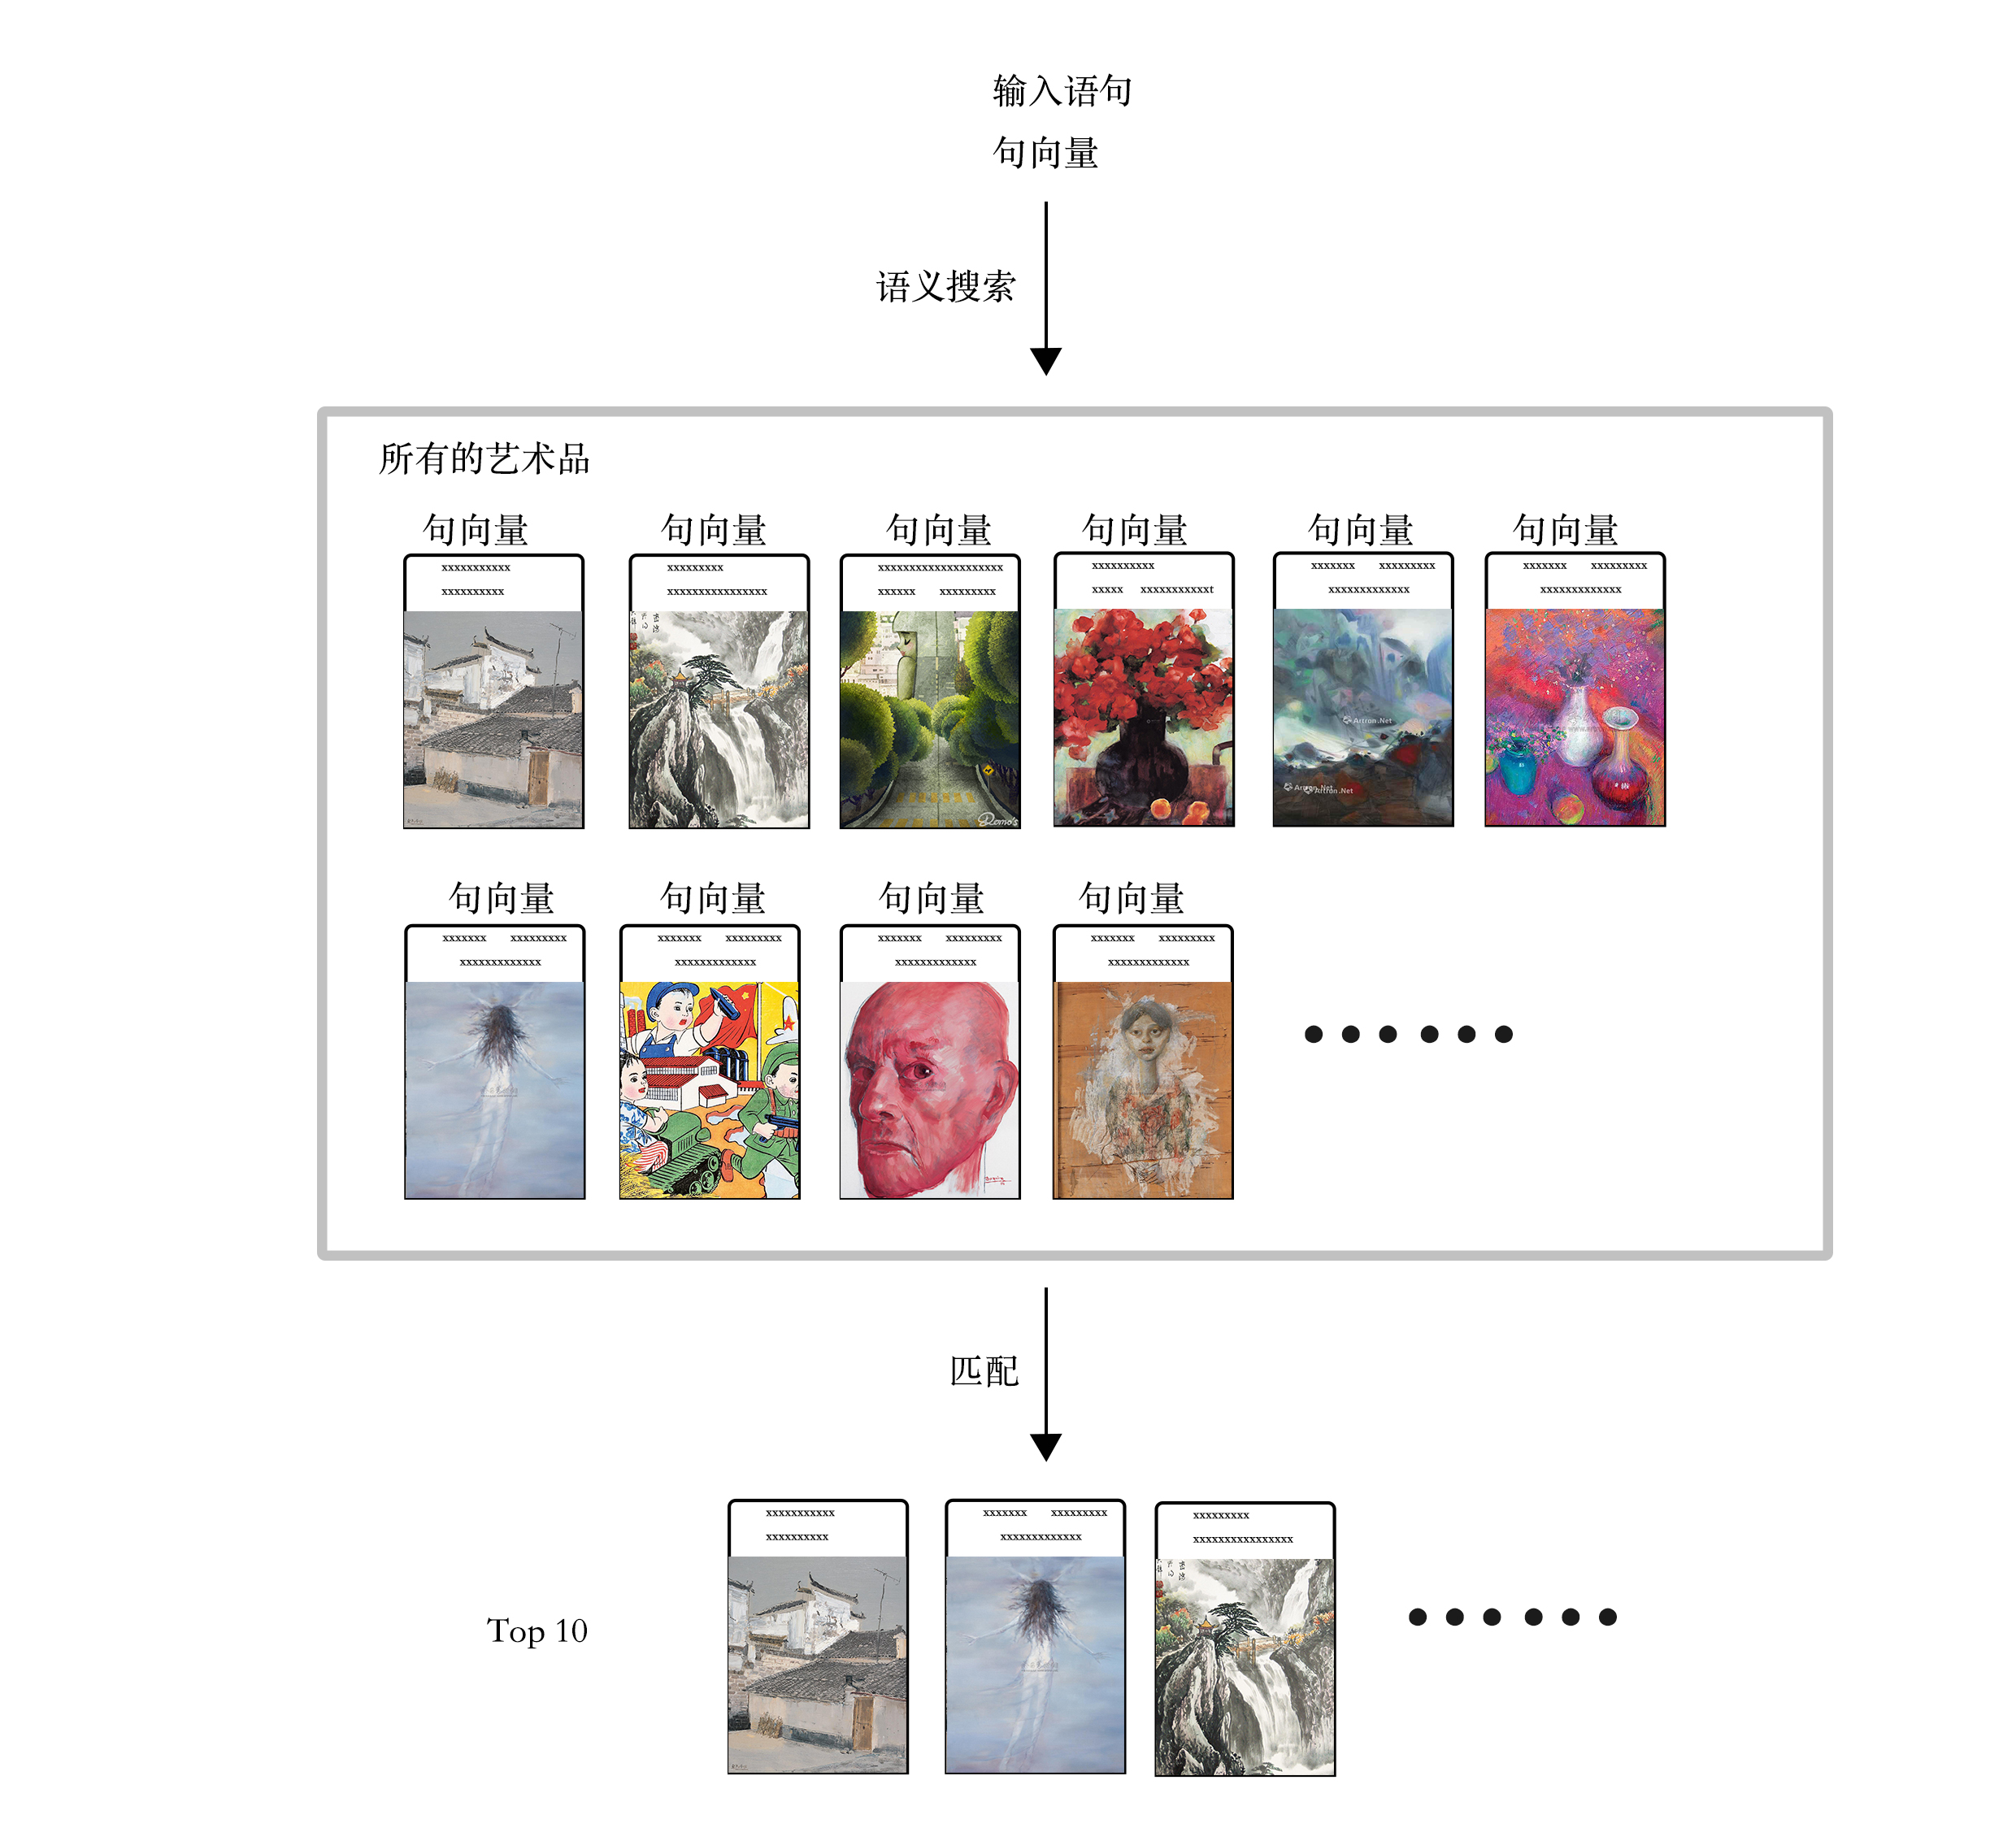
\includegraphics[width=\linewidth,keepaspectratio]{data/chapter-1/搜索.jpg}
\caption{匹配范围}
\label{figure:搜索}
\end{figure}

表征向量的相似度使用余弦相似度。词向量和句向量都经过归一化,向量指向同一方向即为匹配,也就是说向量之间的距离大小即为夹角的大小。如图~\ref{figure:余弦相似度}当两个向量指向相同,余弦为1,两个向量正交,余弦为0,指向相反余弦则为-1。两个向量夹角的余弦值可以确定两个向量是否大致指向相同的方向,故而考量输入向量与艺术品向量的距离使用余弦相似度。\cite{DBLP:journals/corr/abs-1802-09914}

\begin{figure}[!htbp]
\centering
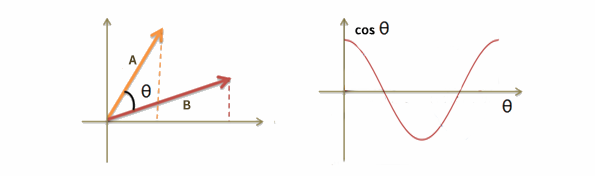
\includegraphics[width=\linewidth,keepaspectratio]{data/chapter-1/1-1.png}
\caption{余弦相似度}
\label{figure:余弦相似度}
\end{figure}

余弦相似度不仅对于二维向量适用,对于任何空间中度向量都适用。

$$ similarity = cos(\theta)= \frac{\vec{A}\cdot\vec{B}}{\|A\| \cdot \|B\|} = \frac{\sum_{i=0}^{n}{A_i \times B_i}}{\sqrt{\sum{{A_i}^2}} \times \sqrt{\sum{{B_i}^2}}}$$

本系统中的词向量和句向量维度为三百,对于归一化之后的句向量来说,所有的句向量的模都是1,即$\|A\| = \|B\|=1$,则

$$ similarity = cos(\theta)=  \sum_{i=0}^{300}{A_i \times B_i} = \mathbf{A} \times \mathbf{B^T}$$

对输入语句的句向量与每个艺术品语句的句向量做矩阵乘法,结果最接近1的就是最匹配的艺术品语句向量,此艺术品的语句和输入语句在语义上是最接近的,由此决定此艺术品就是与输入的语句最匹配的艺术品。\cite{ravichandran2005randomized}接下来就从这个艺术品来提取特征。

在本系统中还为了特定的需求进行一些搜索优化。由于本系统最终是为了从艺术品提取色彩,所以降低色彩很少的作品被搜索到的概率。比如对于书法作品,一般并没有色彩可以用于提取。搜索概率高的艺术类型设置为摄影、综合媒材、水粉水彩、油画、版画,以绘画作品为主。

由于艺术品和文字表达的模糊性,有时文字信息匹配度最高度艺术品事实上并不完全匹配,这种情况的出现往往是由于艺术家为了某些内涵,让艺术品的命名与艺术品内容表面上并不相关,或者艺术品的介绍过于偏重作者的家世、背景,与艺术品的内容关联度很低。为了解决这样的问题,在匹配的过程中,输入语句后,本系统取相似度前10的艺术品作为候选,随机选定其中一件作品提取色彩,当用户不满意当前匹配的色彩可以通过重复点击进行切换,用户也可以选择进入页面进行选择。

\section{色彩提取}

\subsection{系统结构之色彩提取}

由于艺术品的图片和文本语义信息的关联,艺术品图像风格的偏序特性保持到语义描述的偏序特性中,当输入语句和艺术品语句匹配成功后,自然就得到了与输入语句匹配的艺术品的图像。从艺术品图像中提取色彩特征,就可以得到相匹配的色彩方案。

\begin{figure}[!htbp]
\centering
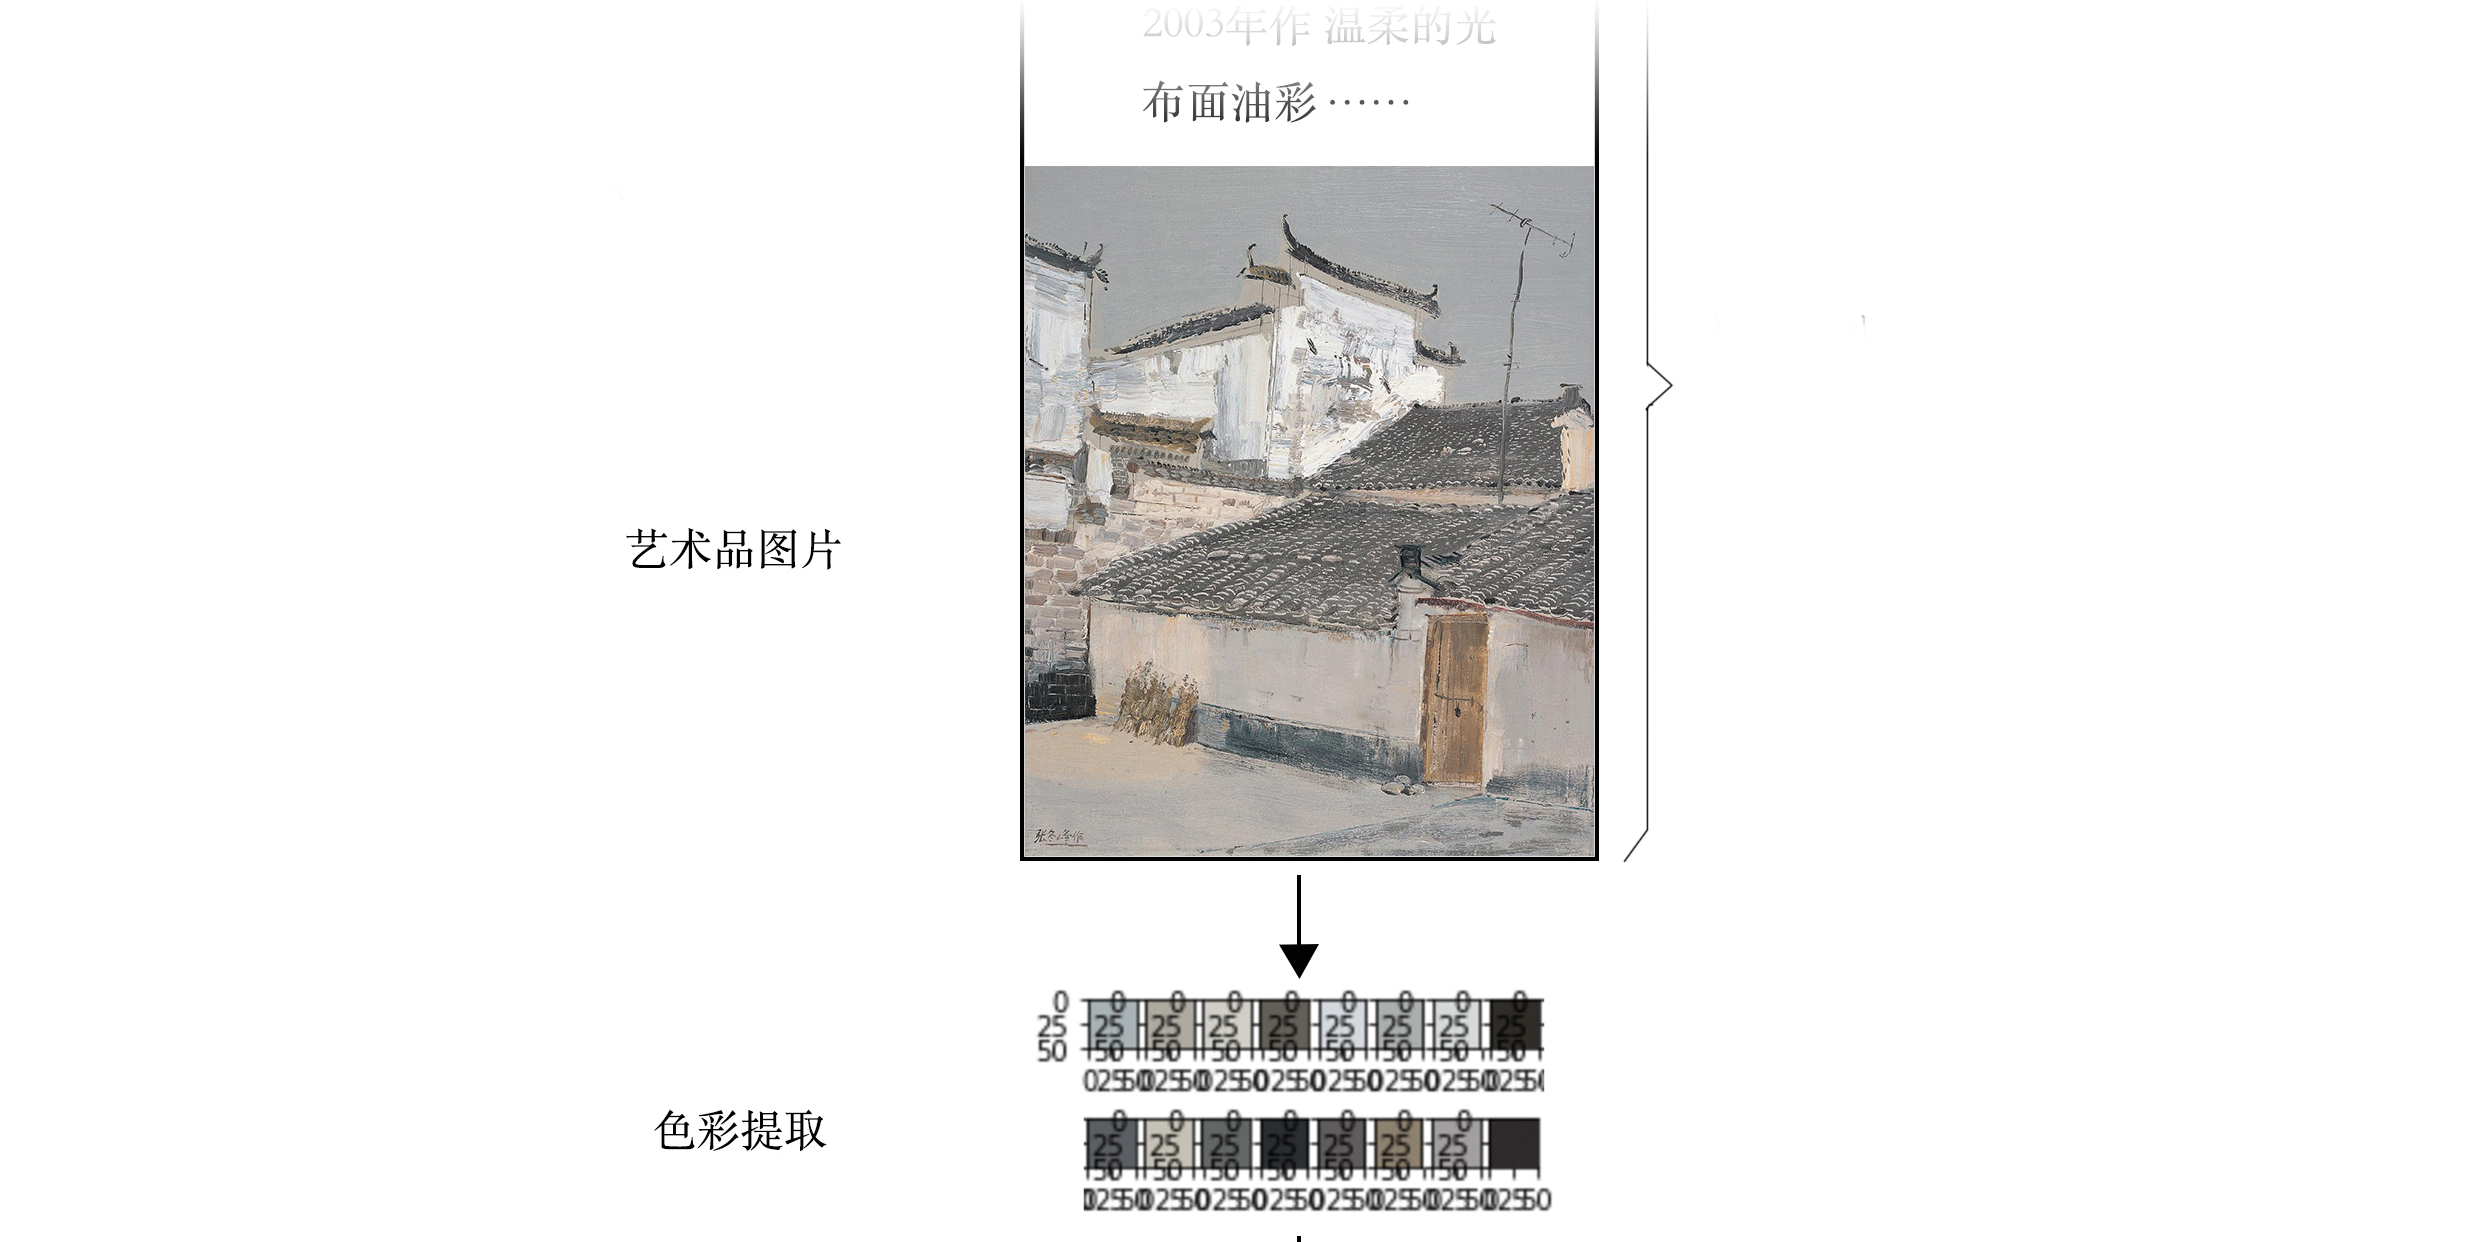
\includegraphics[width=\linewidth,keepaspectratio]{data/chapter-1/系统内部逻辑提取.jpg}
\caption{第二步:提取色彩}
\label{figure:系统内部逻辑提取}
\end{figure}

这一步输出的色彩方案使用RGB色彩模式,每个颜色包括Red-Green-Blue三个通道的值和该颜色本来在艺术品中占的比例(面积比例)。从艺术品图片中占比例最大的颜色开始,可以自定义提取颜色的个数,在本文的测试中取颜色的个数为16。

对于用户来说,输入文本并搜索将会出现一组色彩方案,这个色彩方案来自文本相似度与输入文本排前10的艺术品之一,用户可以通过不改变输入文本,再次搜索,从相似度前10的艺术品中另外随机选择一件,也可以直接打开相似度前10的所有色彩方案手动选择。如图~\ref{figure:搜索结果}虚线框中为文本相似度与输入文本排前10的艺术品,这些内容不展示给用户,用户仅仅关注色彩方案,通过重新搜索,或进入10个色彩方案可以选择。

\begin{figure}[!htbp]
\centering
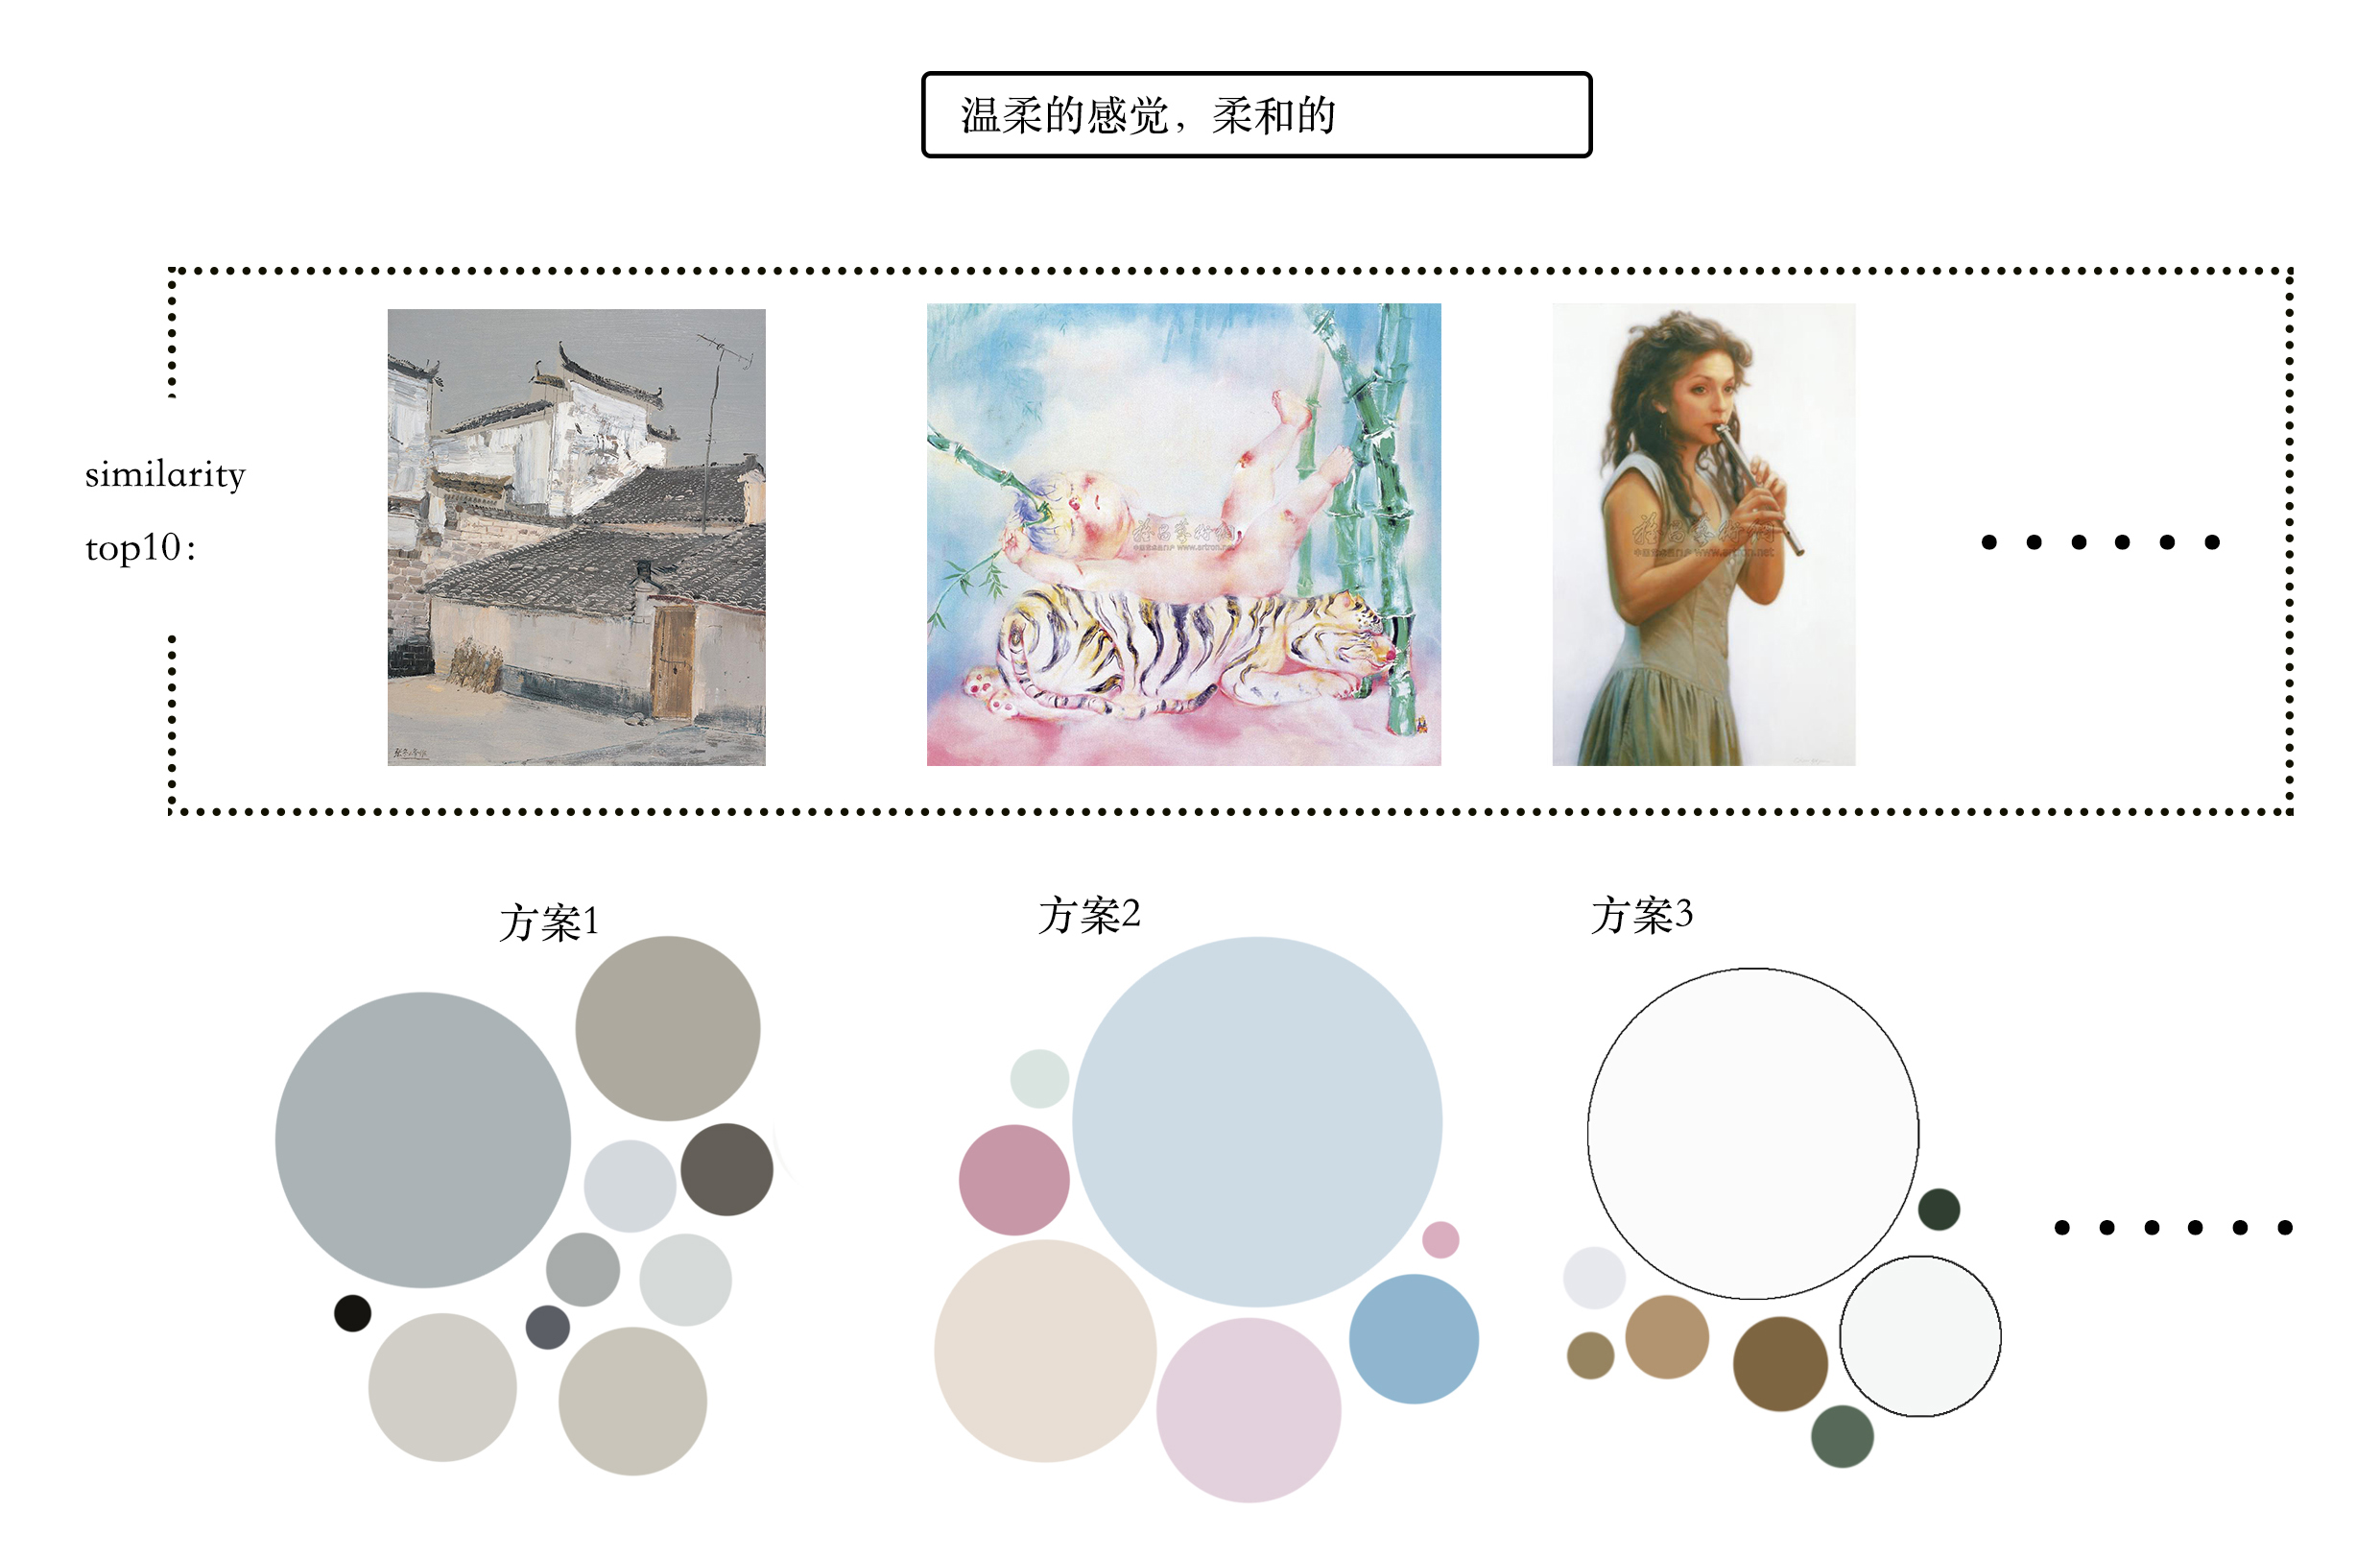
\includegraphics[width=\linewidth,keepaspectratio]{data/chapter-1/搜索结果.jpg}
\caption{备选方案}
\label{figure:搜索结果}
\end{figure}

\subsection{色彩模式}

颜色是不同波长的可见光进入人类的眼睛,由视锥细胞感受到不同波长的比例传到大脑所产生的感受。可见光的波长变化3-5nm,人类就可以分辨为不同的颜色,要对色彩进行数字编码,可以使用多种方法。\cite{colormodel}

RGB色彩模式指Red-Green-Blue三种色光的混合。人类有三种视锥细胞,分别对红、绿、蓝三种色光最为敏感,所以人类的眼睛可以看到的色彩都是由这三种颜色的光经不同比例构成的。光的混合在牛顿时代就被发现了,使用红、绿、蓝三种色适当混合,可以引起光谱上所有任何颜色的感觉,三原色混合原理广泛地应用于照相、显示技术中。数字化常见的颜色标准也使用红、绿、蓝三个通道混合,称为RGB色彩模式。通常情况下,RGB各有256级亮度,用数字表示为从0、1、2...直到255。比如(255,0,0)指红色,(255,255,0)则是黄色,(0,0,0)是三种色光的亮度都为0,即黑色,(255,255,255)是三种色光的亮度都为最高,混合起来为白色。在计算机领域RGB色彩模式是很常用的,需要注意的是,在编码时有时会使用BGR模式,意思并没有区别,但是数字的顺序是反过来的,RGB(255,0,0)为红色而BGR(255,0,0)为蓝色。

常用的色彩模式还有CMYK,多用于印刷,CMYK同样将颜色分为数个通道混合,但是通道为Cyan(青色)-Magenta(品红)-Yellow(黄色)-black(黑色)四个,这四种颜色的染料可以调配出几乎所有颜色。CMYK和RGB色彩模式可以相互转化,转化的方式如下。

\begin{python}
def rgb_to_cmyk(r,g,b):
	cmyk_scale = 100
    if (r == 0) and (g == 0) and (b == 0):
        # black
        return 0, 0, 0, cmyk_scale
    # rgb [0,255] -> cmy [0,1]
    c = 1 - r / 255.
    m = 1 - g / 255.
    y = 1 - b / 255.

    # extract out k [0,1]
    min_cmy = min(c, m, y)
    c = (c - min_cmy) / (1 - min_cmy)
    m = (m - min_cmy) / (1 - min_cmy)
    y = (y - min_cmy) / (1 - min_cmy)
    k = min_cmy

    # rescale to the range [0,cmyk_scale]
    return c*cmyk_scale, m*cmyk_scale, y*cmyk_scale, k*cmyk_scale
\end{python}

关于图像等OpenCV、PIL等库都能够进行转化。在本系统中,所有的色彩都按照RGB模式编码,不同的色彩模式需要进行转化。

\subsection{色彩提取}

色彩提取从图片中占比例最大的颜色开始,可以自定义提取颜色的个数$N_color$,输出的每个颜色包括Red-Green-Blue三个通道的值和该颜色本来在艺术品中占的比例(面积比例)。

色彩提取的算法采用色彩梯度算法。使用RGB色彩模式。首先为了减小计算量通过压缩图像生成一个略缩图。将R-G-B各分为步长为step的n个等级,即总共有$n^3$个颜色等级。对每个颜色等级的像素点个数进行计数,定义色彩c的分数为$score(c) = (saturation(c) + 0.1) \times count(c) $,其中$saturation(c)$为色彩的饱和度,$count(c)$则为颜色为x的像素点个数。非常接近白色的颜色(RGB三个参数均大于200的颜色)和非常接近黑色的颜色(三个参数均小于50的颜色)都不参加评分。面积越大、色彩饱和度越高,则色彩得分越高。得分越高的颜色就是图片中主要的颜色,提取前$N_color$个得分最高的颜色,$count(c)$就代表这这个颜色在艺术品中占的比例。

\begin{python}
def get_dominant_color(image, beside_color, step):  
      
#颜色模式转换,以便输出rgb颜色值  
    image = image.convert('RGBA')  
      
#生成缩略图,减少计算量 
    image.thumbnail((200, 200))  
      
    max_score = 0 
    dominant_color = 0  
    proportion = 0
        
    for count, (r, g, b, a) in image.getcolors(image.size[0] * image.size[1]):  
        # 跳过透明色  
        if a == 0:  
            continue
        # 跳过白色    
        if ((r>180)&(g>180)&(b>180)):  
            continue
        # 跳过黑色   
        if ((r<80)&(g<80)&(b<80)):  
            continue 
            
        if ((beside_color[0]-step<r<beside_color[0]+step)&(beside_color[1]-step<g<beside_color[1]+step)&(beside_color[2]-step<b<beside_color[2]+step)):  
            continue
               
        saturation = colorsys.rgb_to_hsv(r / 255.0, g / 255.0, b / 255.0)[1]          
        y = min(abs(r * 2104 + g * 4130 + b * 802 + 4096 + 131072) >> 13, 235)         
        y = (y - 16.0) / (235 - 16)  
          
        # 忽略高亮色  
        if y > 0.9:  
            continue  

        score = (saturation + 0.1) * count  
          
        if score > max_score:  
            max_score = score  
            dominant_color = (r, g, b)  
            proportion = count
      
    return dominant_color, proportion  
\end{python}

这样的方式略过黑色和白色(或者说几乎是黑色和白色的颜色),面积越大、色彩饱和度越高,色彩越排在前面,可以完全忠实于艺术品图片提取色彩。

\section{上色算法}

\subsection{系统结构之自动上色}

从艺术品中提取色彩之后,色彩方案可以自动在效果图线稿上预览。上色预览主要是为了让设计师直观的到色彩方案的风格和潜力,为了满足这个目标有3点需求:1.快速实时;2.色彩准确和比例较准确;3.效果图清晰明确。

\begin{figure}[!htbp]
\centering
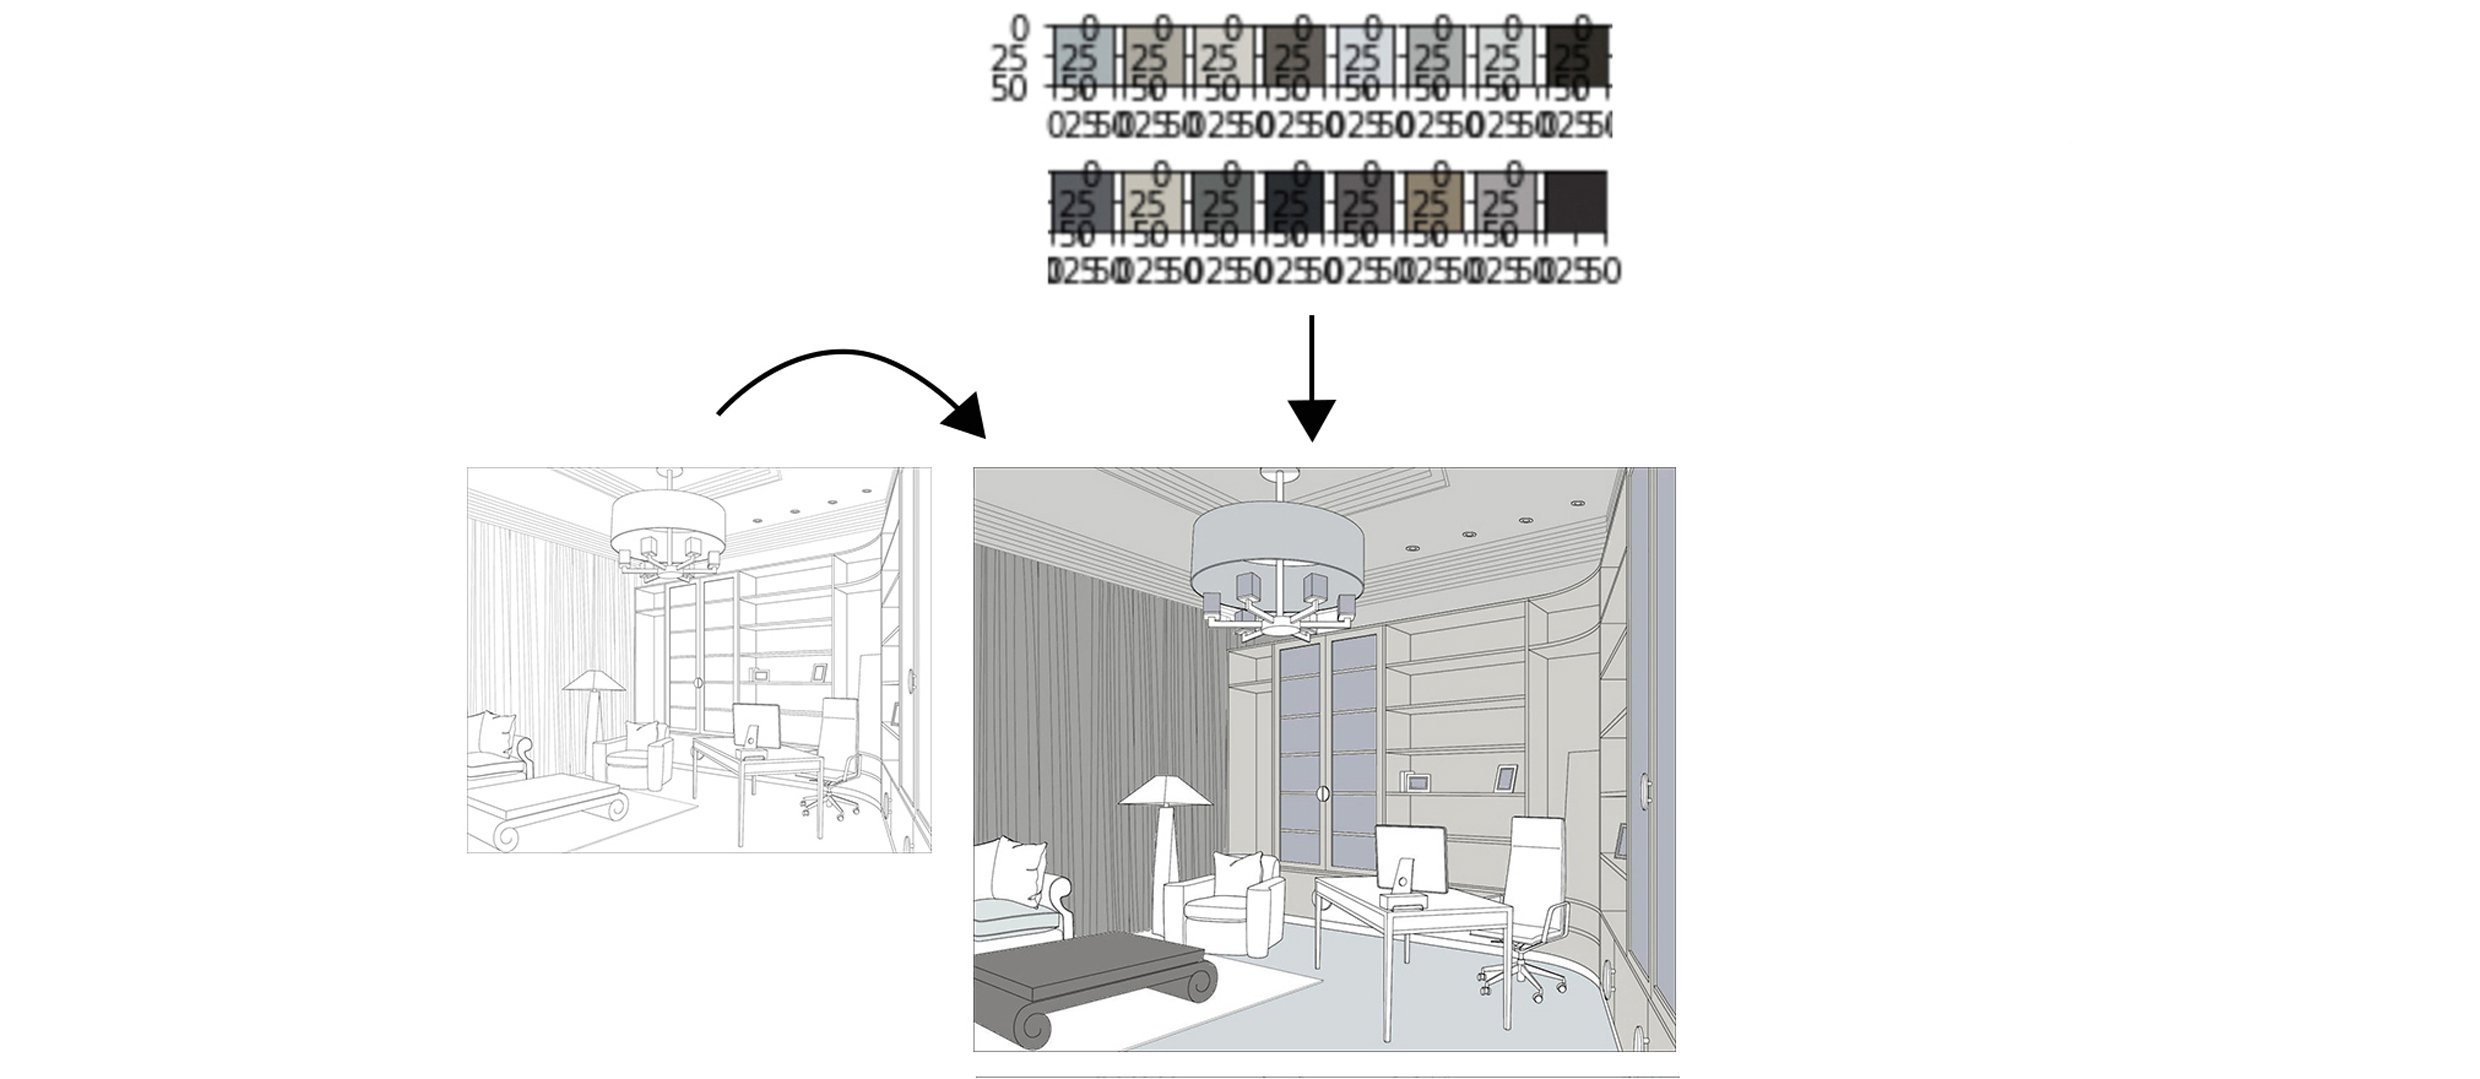
\includegraphics[width=\linewidth,keepaspectratio]{data/chapter-1/系统内部逻辑3.jpg}
\caption{第三步:自动上色}
\label{figure:系统内部逻辑提取}
\end{figure}

系统准备了室内设计,服装设计各1套效果图线稿预览,之后的测试发现,对于上色区域占图片比例较小并且色彩有限的服装、产品效果图本系统也可以使用,但系统效果更适合室内设计效果图。每次生成的预览效果图由于有随机性的参与都不可复制,但可以使用同一色彩方案生成不完全一致但风格同一的预览图。

\subsection{泛洪填充算法}

泛洪填充算法(Flood Fill Algorithm)又称漫水填充算法,是在很多图形绘制软件中常用的填充算法。\cite{floodfill} 泛洪填充算法可以为图像的封闭区域填充颜色,成完整的填充需要的条件有两点:1.该区域有封闭的边界;2.该区域的像素点色彩相同。如图~\ref{figure:泛洪填充}。

\begin{figure}[!htbp]
\centering
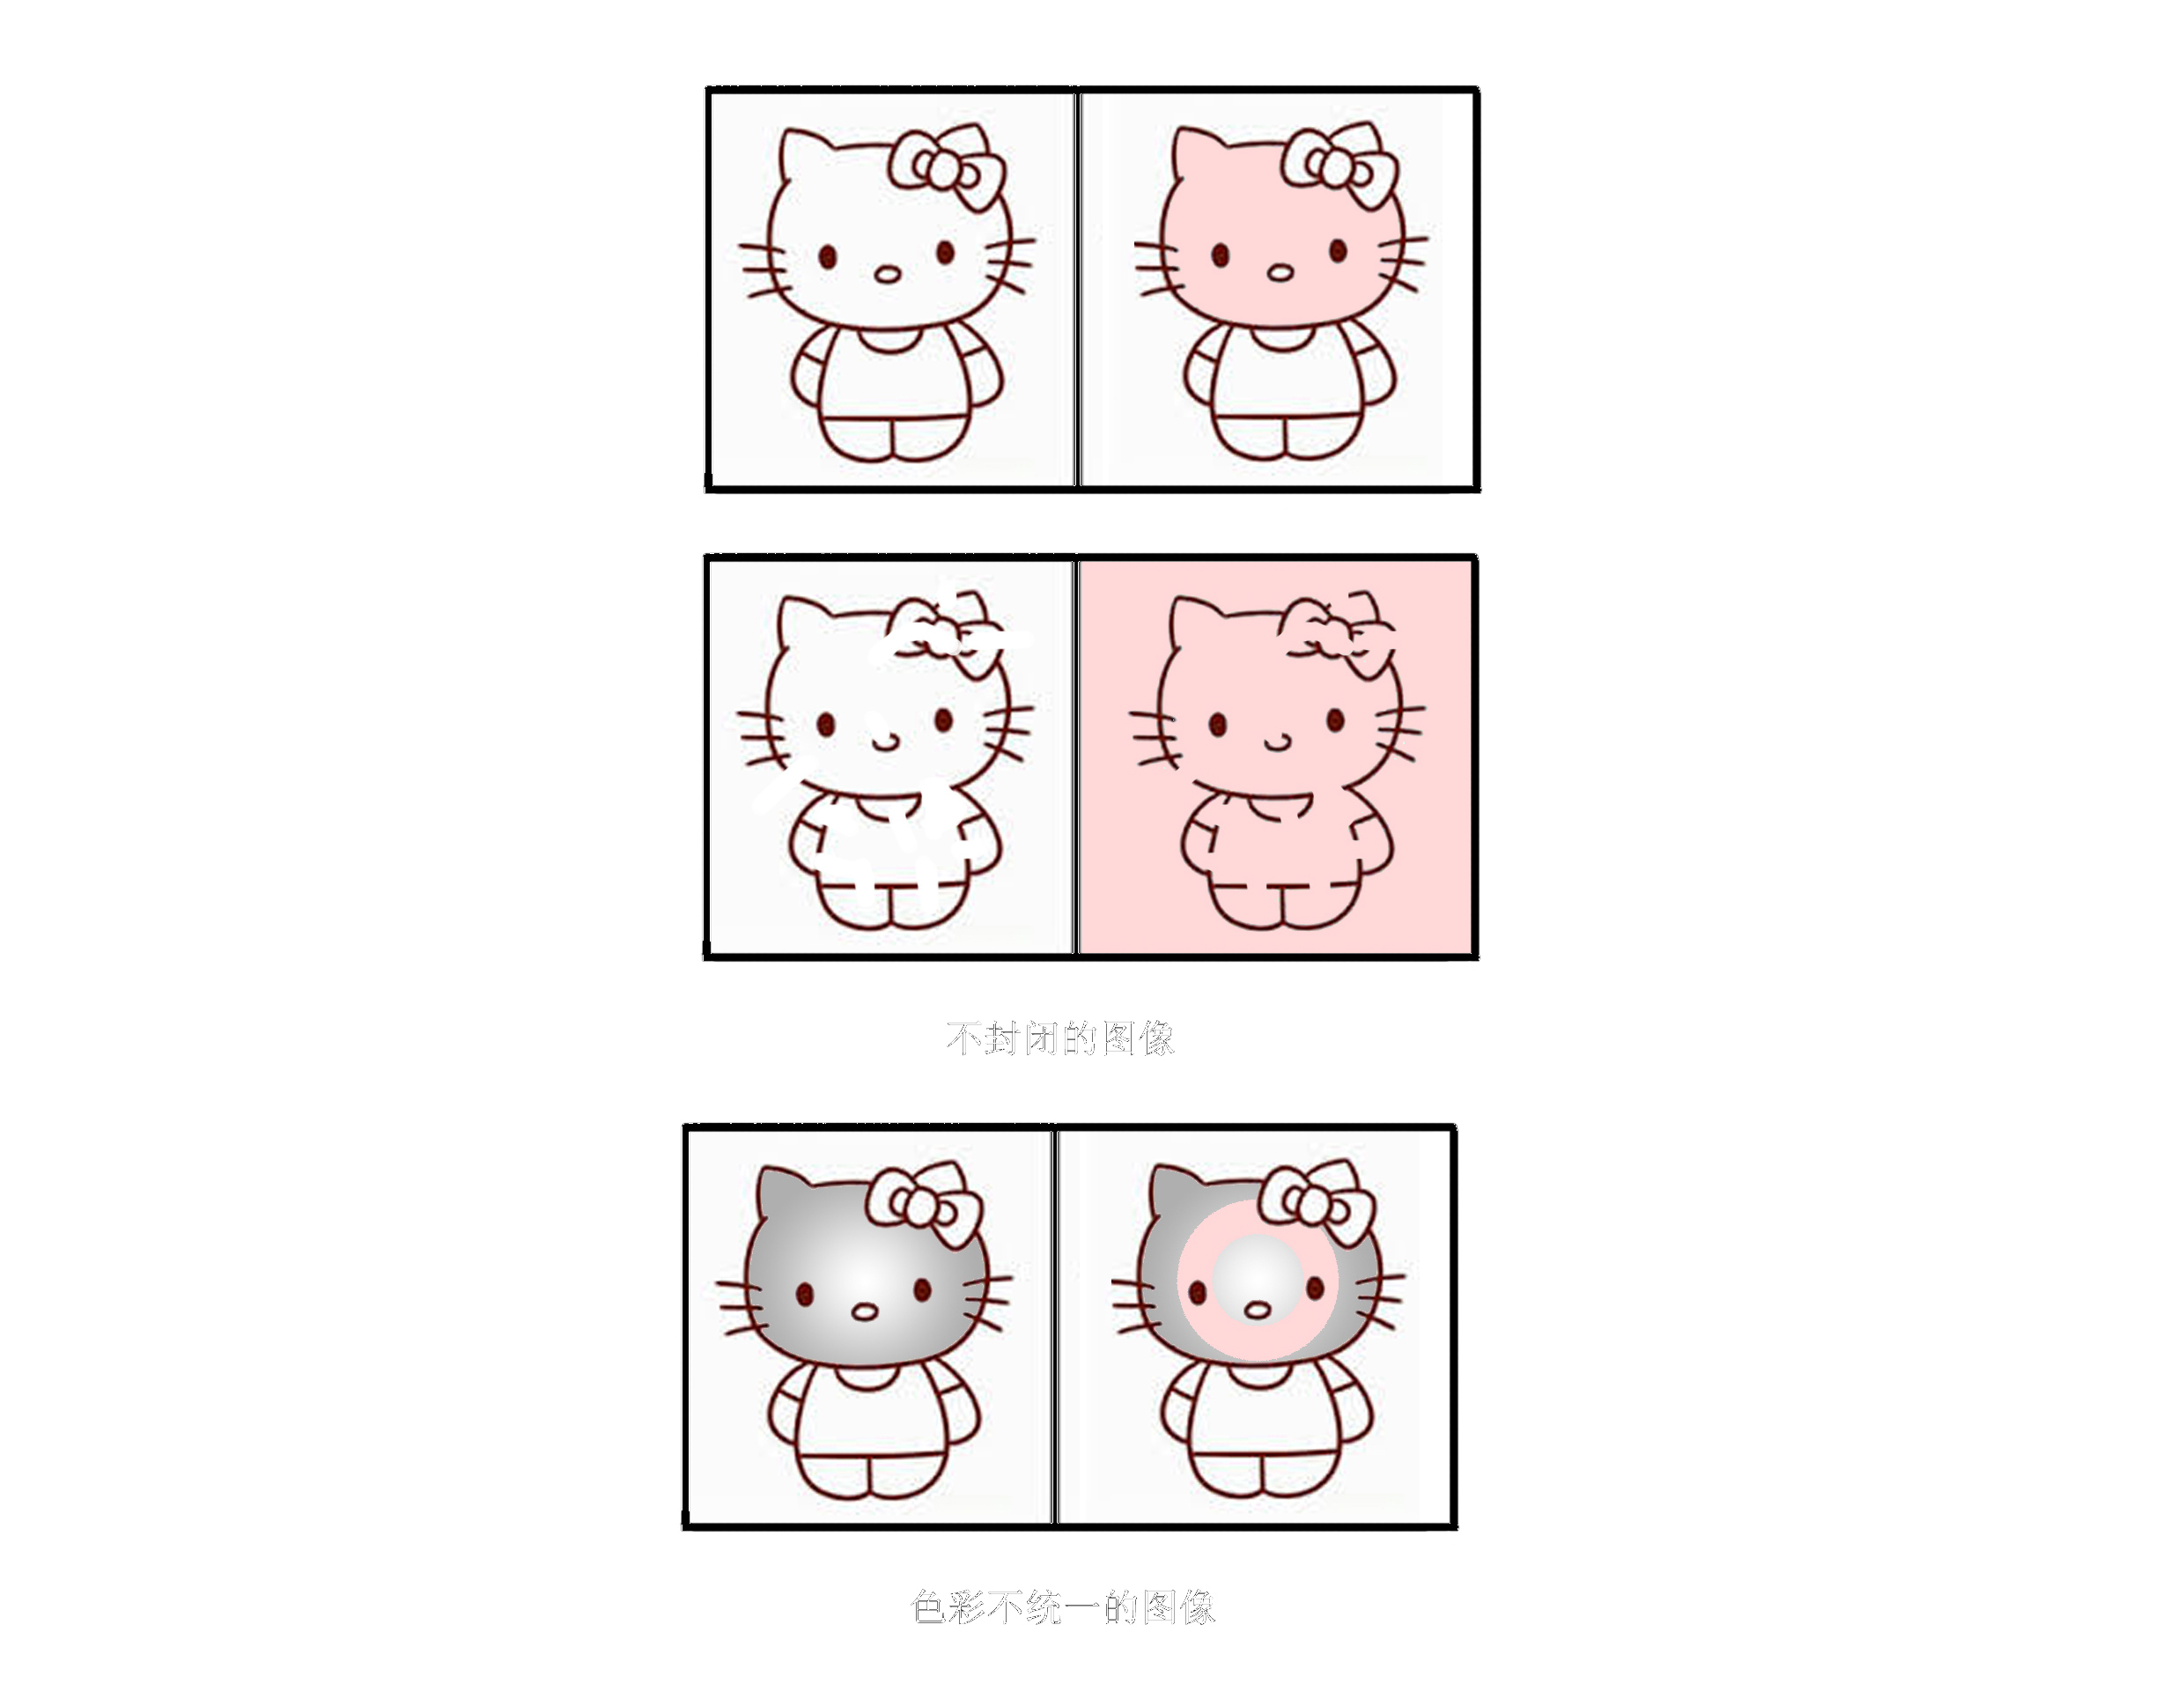
\includegraphics[width=\linewidth,keepaspectratio]{data/chapter-1/kitty.jpg}
\caption{泛洪填充}
\label{figure:泛洪填充}
\end{figure}

泛洪填充算法的原理是,要为某个区域填充色彩a,在这个区域中取一个像素点,这个点被称为种子点,种子点原始的颜色为x,将种子点的色彩从x改为a,对于所有相邻且颜色为x的点也都染色为a,染色后的点相邻且颜色为x的点也都染色为a,一直传播下去,直到这个区域内所有的点都被填充完为止。如图~\ref{figure:填充过程}。

\begin{figure}[!htbp]
\centering
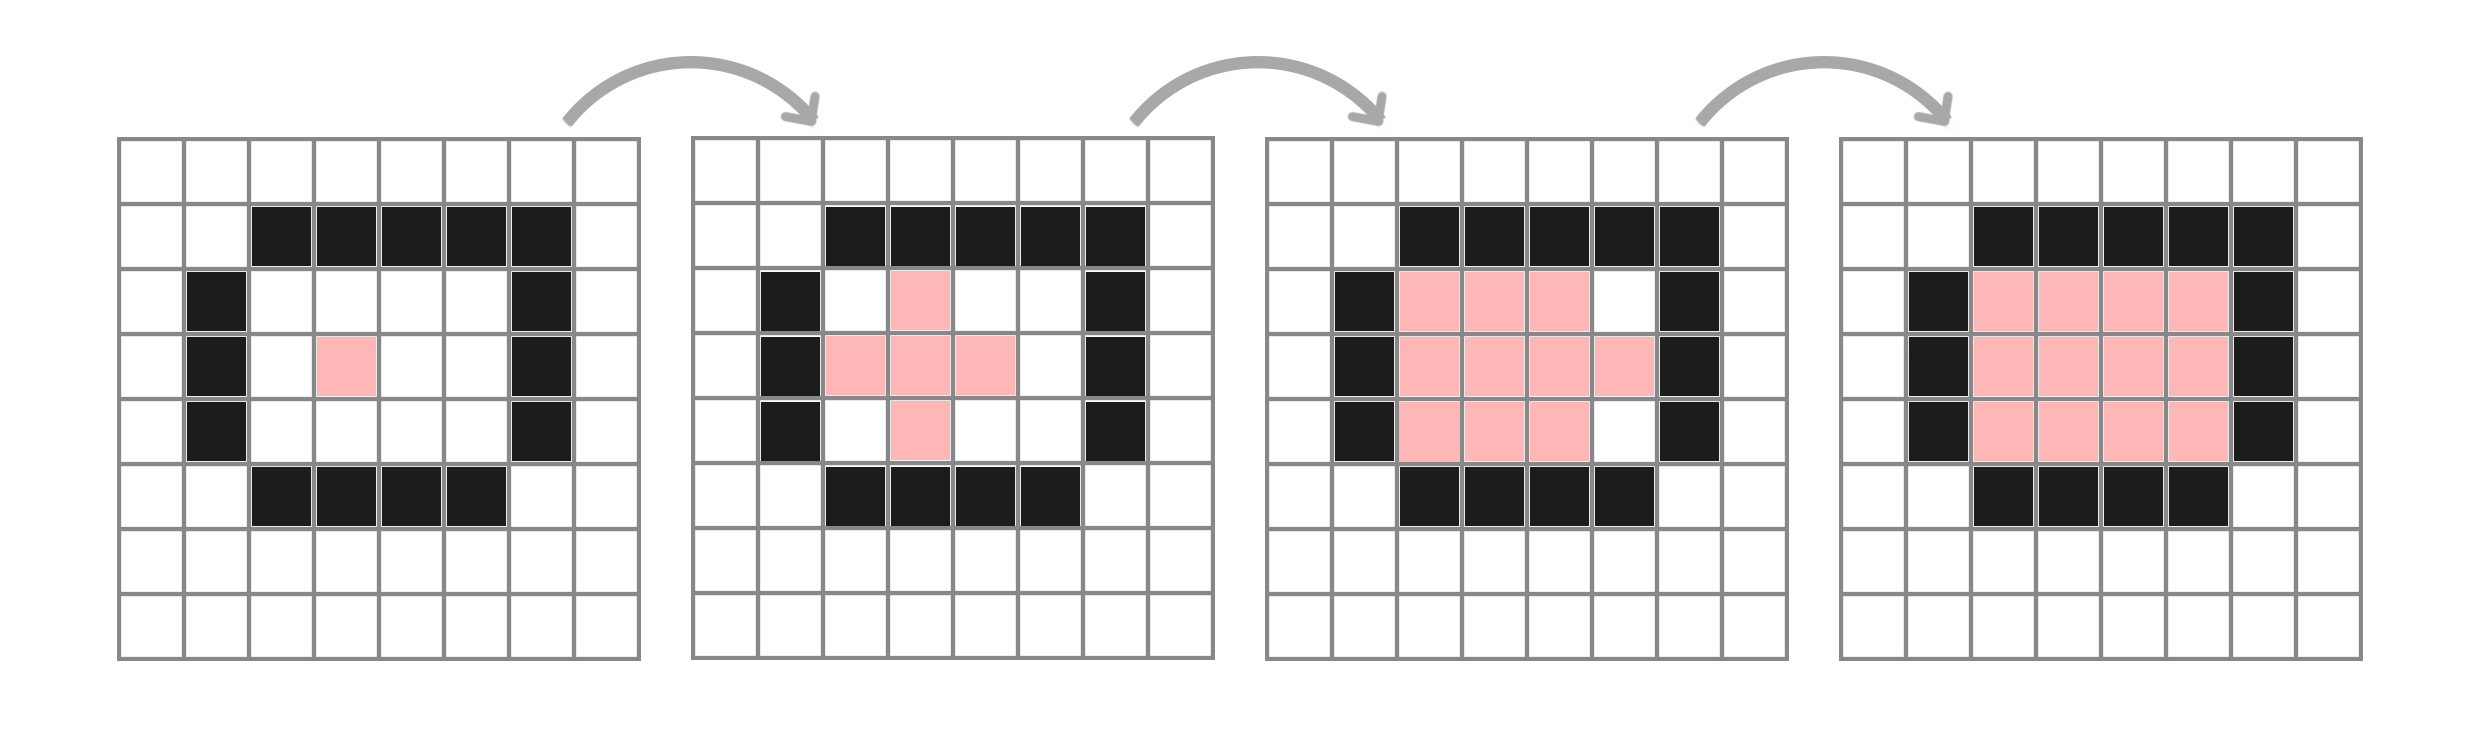
\includegraphics[width=\linewidth,keepaspectratio]{data/chapter-1/填充.jpg}
\caption{填充过程}
\label{figure:填充过程}
\end{figure}

实现这样的算法只需要最基础的递归算法或堆栈算法。即
\begin{python}
def floodfill(x, y, oldColor, newColor):
    # assume surface is a 2D image and surface[x][y] is the color at x, y.    
    if surface[x][y] != oldColor: return # the base case
    surface[x][y] = newColor
    floodfill(x + 1, y, oldColor, newColor) # right
    floodfill(x - 1, y, oldColor, newColor) # left
    floodfill(x, y + 1, oldColor, newColor) # down
    floodfill(x, y - 1, oldColor, newColor) # up
\end{python}

在实际的使用中,这个简单的算法还需要一些改进。复制制作一个遮罩层,以防图片被直接改变导致返回结果不正常。加入容差的概念,即当染色点原始的颜色为最大负差值不超过RGB(20,20,20),最大正差值不超过RGB(50,50,50),则可以扩散。

在本系统中,待上色的效果图为室内设计效果图,通过随机选点来为设计效果图上色。每次上色的程序如下:随机选取效果图中像素点,如果这个点为白色则填充当前色彩,同时替换当前色彩为色彩列表下一个色彩;如果这个点非白色,则再次随机选取效果图中的像素点。使用的色彩列表为从艺术品提取的色彩方案,色彩按艺术品中色彩的比例从高到低排序,循环排列,循环多次,直到图片上色完整。

\subsection{一些问题}

\subparagraph{漏掉到小面积——随机游走}:
使用泛洪填充算法可以非常准确工整的为室内设计效果图线稿上色,完全的随机取点会使某些较小的面积被选中的概率太小,所以无法上色的情况严重,如图~\ref{figure:漏掉上色面积的问题以及解决办法}(a)图像中很多地方没有成功上色。

\begin{figure}[!htbp]
\centering
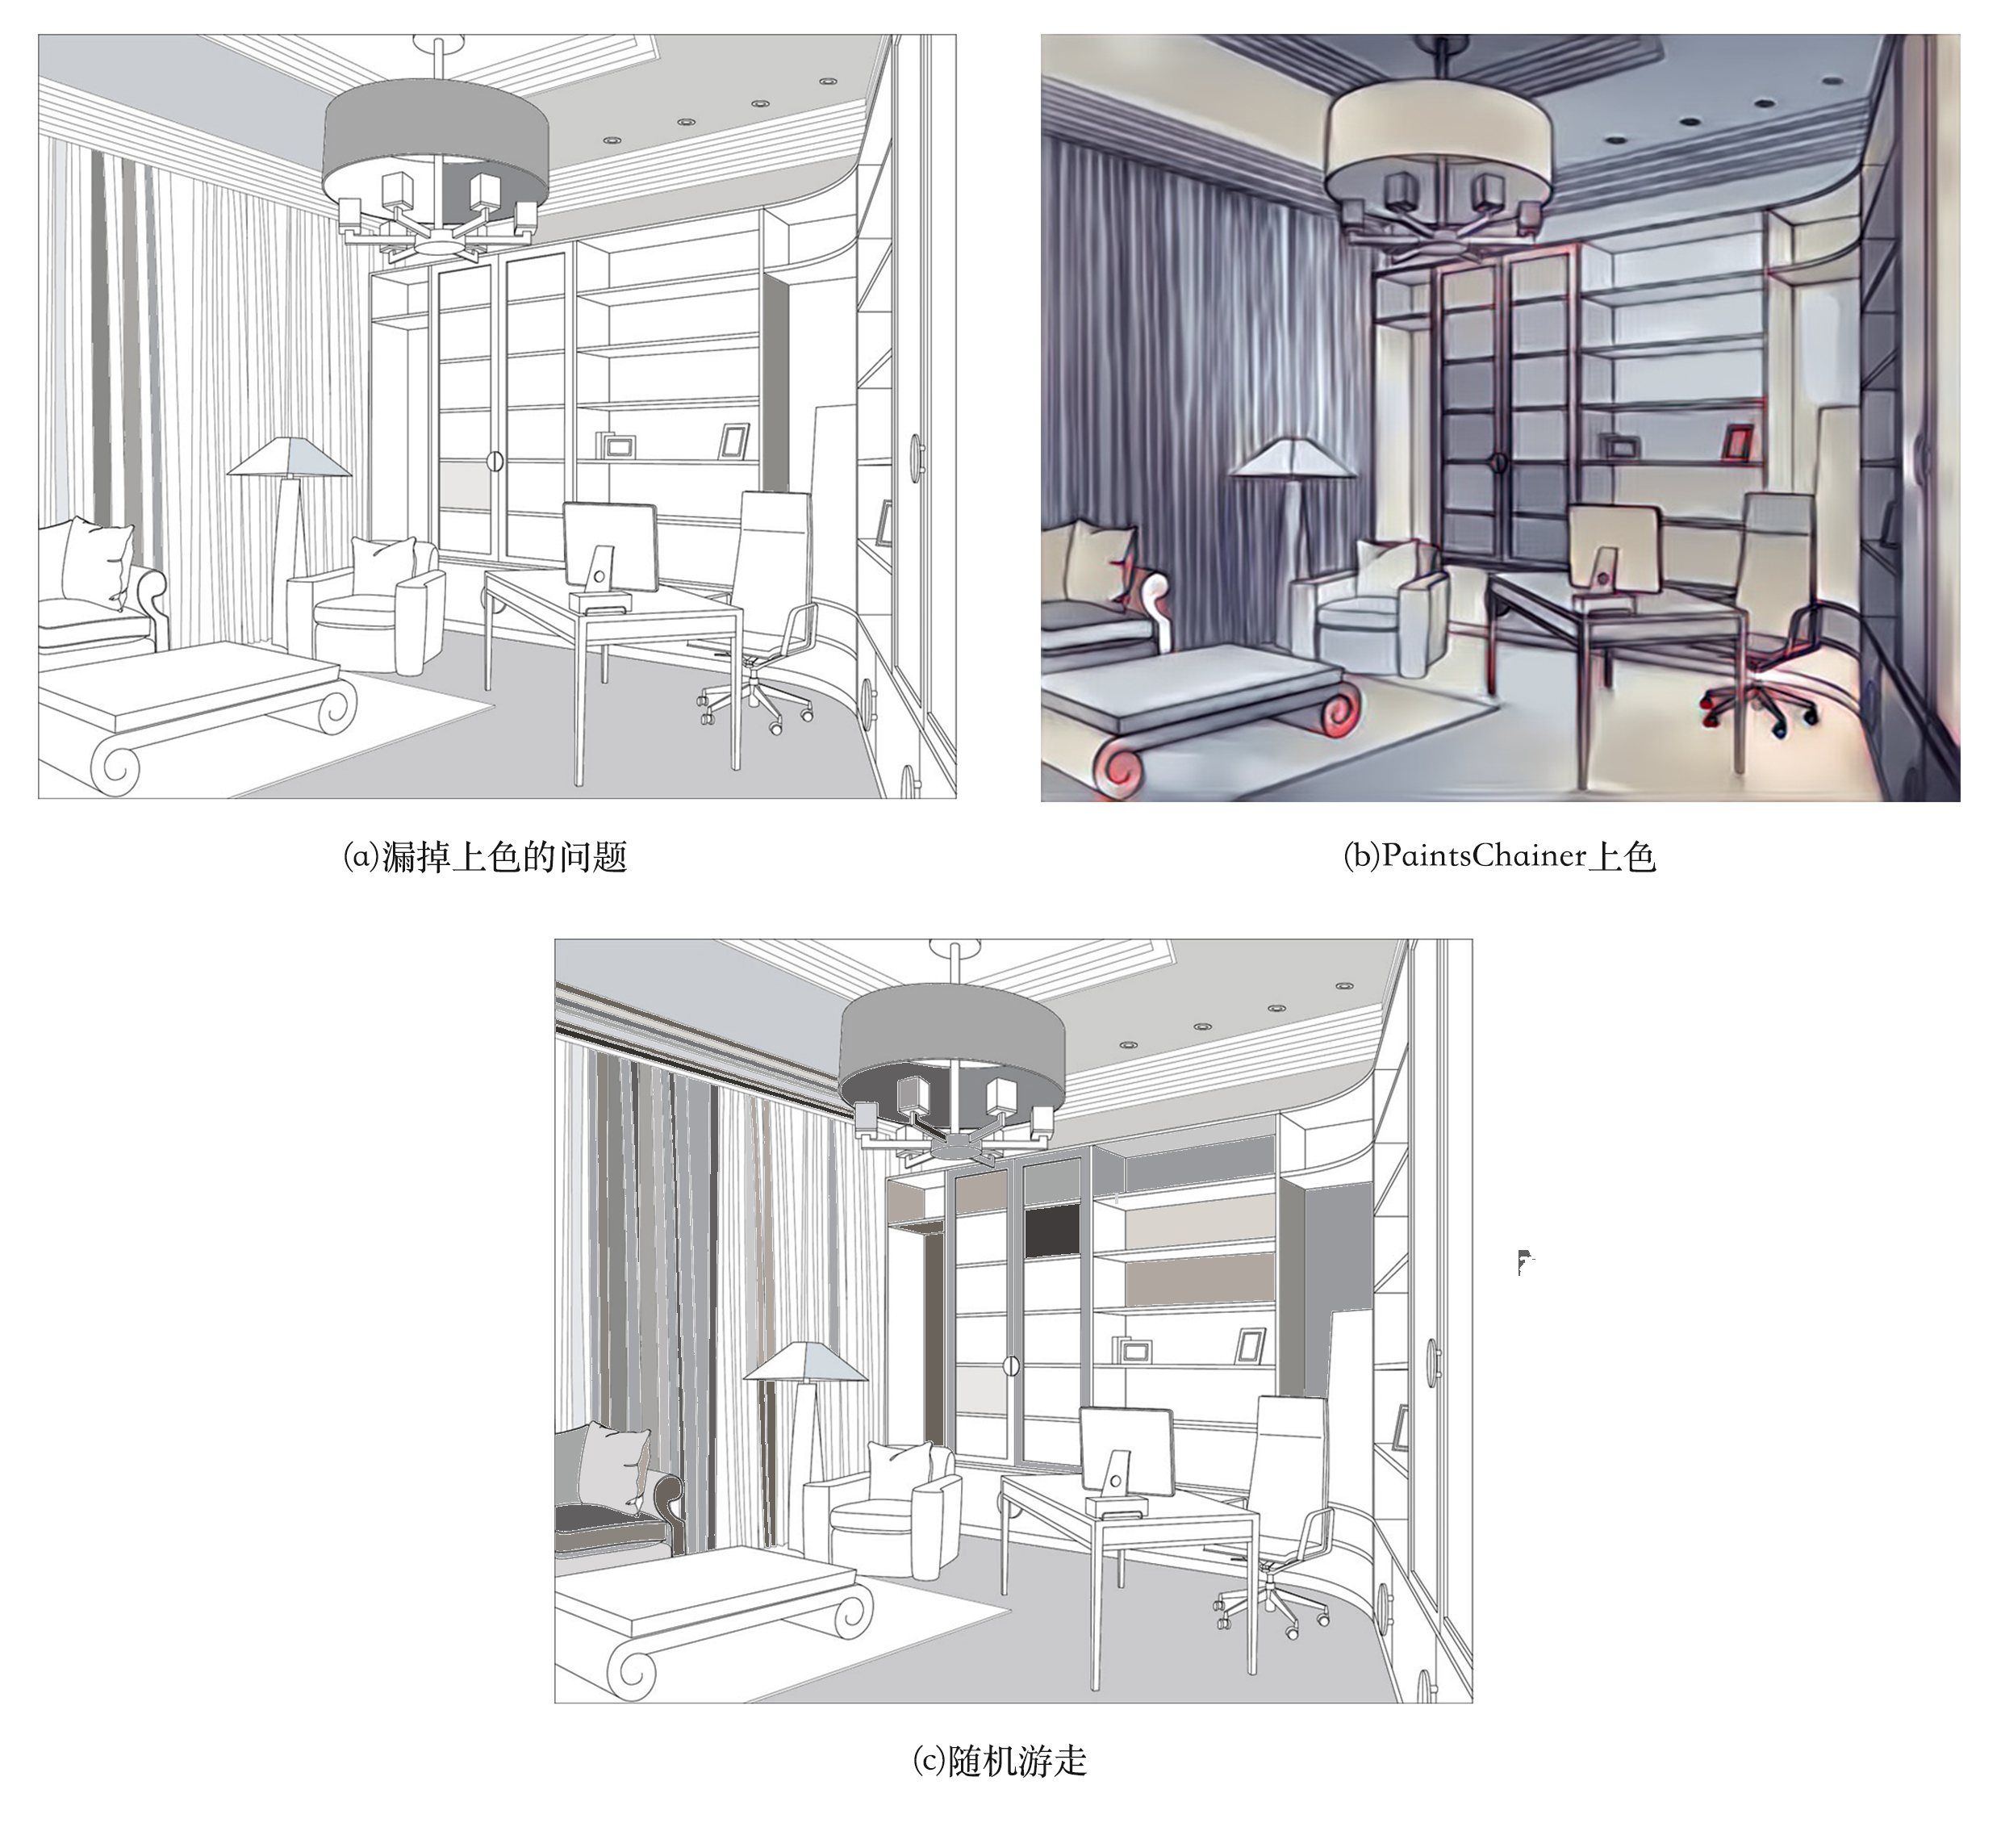
\includegraphics[width=\linewidth,keepaspectratio]{data/chapter-1/预览2.jpg}
\caption{漏掉上色的问题}
\label{figure:漏掉上色面积的问题以及解决办法}
\end{figure}

为了解决这个问题,PaintsChainer所采用的神经网络算法的可以完全的给整张图片上色,如图~\ref{figure:漏掉上色面积的问题以及解决办法}(b)但是对于即时预览色彩方案的效果图来说,不工整的上色、混色、神经网络生成的错误阴影导致预览色彩改变并不适合本系统的需要。生成图像的数十秒延迟也是这个算法不合适的原因。

在原来的方法上面可做一些改进使用随机游走的方式,完全的随机取点会使某些较小的面积被选中的概率太小,无法上色。使用随机游走的方式改进上色算法可以更少出现漏掉面积较小的区域的情况。随机游走的方式倾向于一个区间接一个区间的上色,如图~\ref{figure:漏掉上色面积的问题以及解决办法}(c),循环次数足够多的情况下可以起到更好的效果。

\subparagraph{色彩连续性——图片预处理}:

使用洪填充算法会出现这样的问题,例如区域1和区域2都是天花板,一般而言是同种颜色,但是
现在的填充算法一点也不懂这件事。

\begin{figure}[!htbp]
\centering
\includegraphics[width=\linewidth,keepaspectratio]{data/chapter-1/预2.jpg}
\caption{色彩连续性的问题}
\label{figure:漏掉上色面积的问题}
\end{figure}

所以将这个效果图进行一点预处理,这样可以基本保证在每个完整的物体会填充同一种色彩。预处理的方式是通过标注的方式将同一物体的信息提取出来,删去物体内部的线条,保留物体的的外轮廓。与此同时我们还可以做一些其他的标注,比如将透明的物体的色彩标注为某个灰色。之后再进行填充,就可以将同一个物体填充一个颜色。最后,再通过图层叠加的方式将效果图的原线稿叠加在上色稿上,得到最终的效果图。

\begin{figure}[!htbp]
\centering
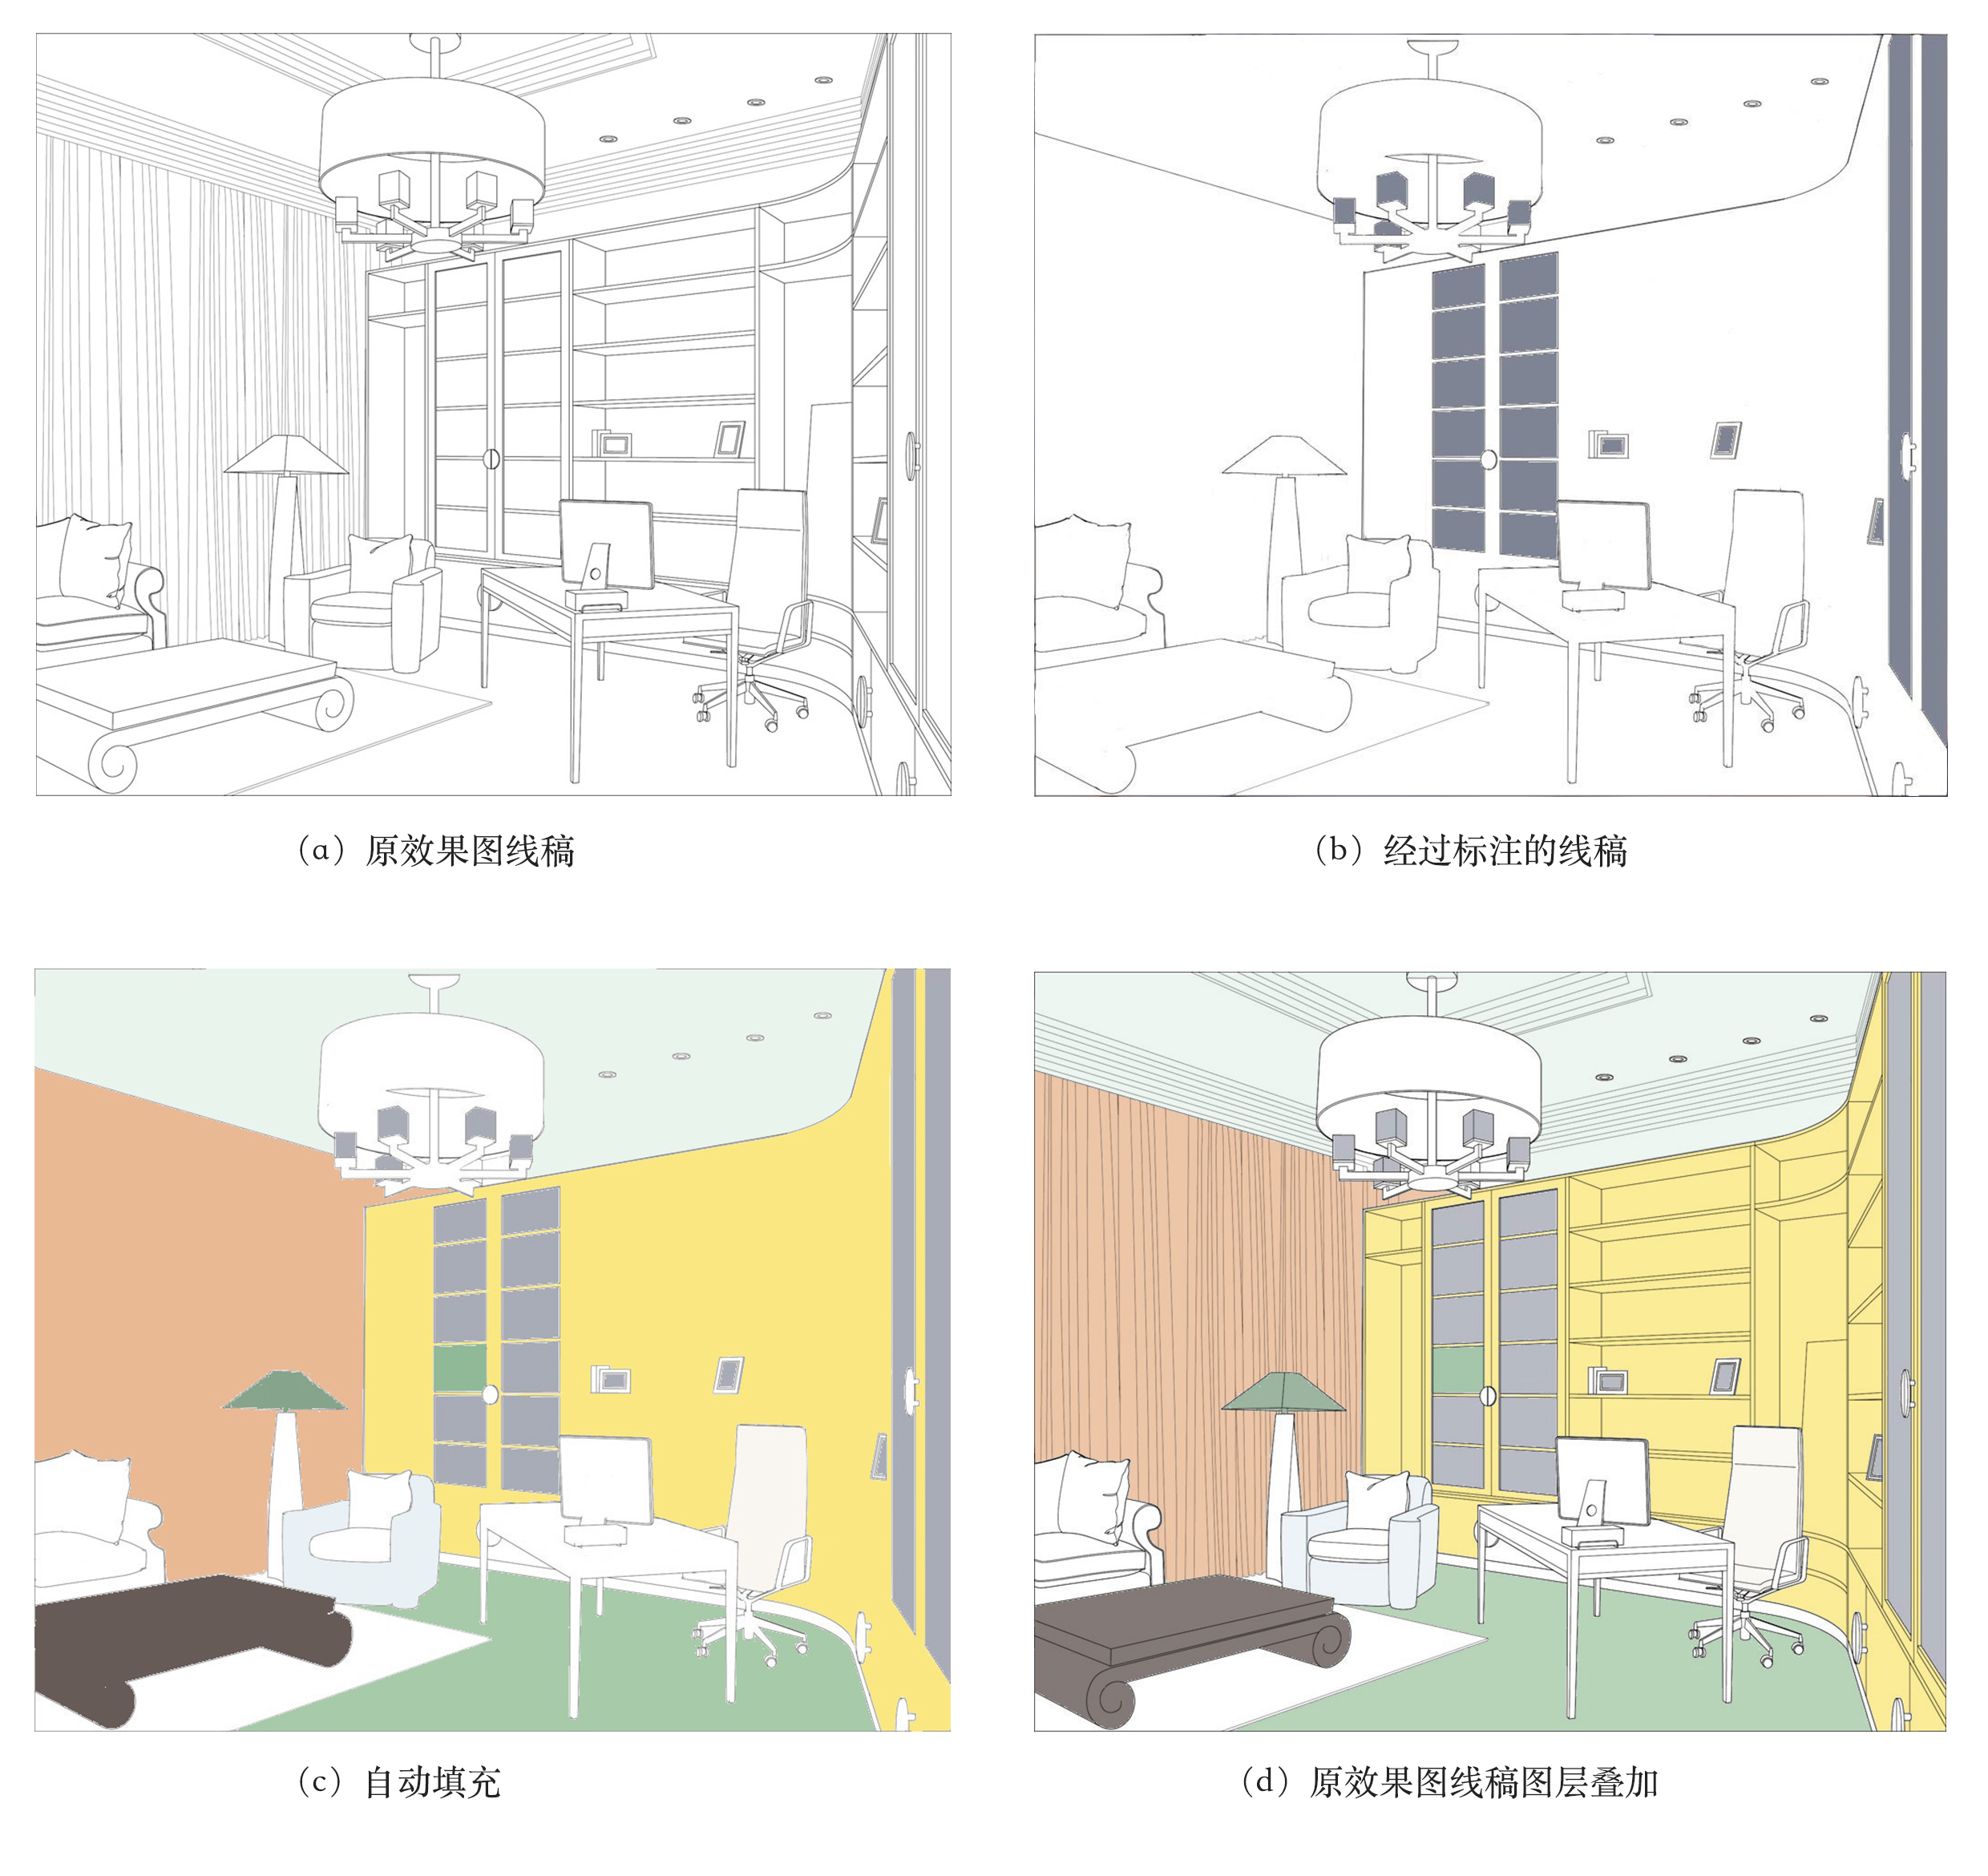
\includegraphics[width=\linewidth,keepaspectratio]{data/chapter-1/预览2副本.jpg}
\caption{色彩连续性的处理}
\label{figure:漏掉上色面积的问题}
\end{figure}


%\subsection{色彩比例}

%对于区域$i$,在效果图上的面积占比为$P_i$,则随机选择种子点在区域$i$的可能性也为$P_i$。对于色彩$j$,在原艺术品上占比例为$p_j$。

\section{本章小结}

本系统的整体思路为:1.输入对需求的文本描述;2.针对输入语句对艺术品的文本信息进行语义搜索,找出与之关联度高的艺术品文本信息;3一句艺术品数据库中艺术品的图片信息和文本信息的隐藏存词关联匹配对应,找出与输入文本关联度高的图片;4.从图片中提取色彩方案,包括绘画作品的色彩和配色比例;5将所提取的色彩运用到设计效果图上预览。

对于用户来说,本系统的使用方式如下:1.用户输入对需求的文本描述;2.得到配色方案;3.当用户不满于当前色彩方案可以重新搜索;4.使用当前色彩方案为效果图上色;5.当用户不满于当前效果图可以使用当前色彩方案重新上色。

在实现的过程中,首先需要解决的是自然语言处理的问题。本系统采用word embedding的方式实现单词向量化,word embedding采用CBOW模型,使用哈夫曼树、负采样优化、fast text等策略加快速度以及增加编码的精度,实现对词语语义信息的提取。词向量到句向量的转化采用加权合成的方法,考虑词频、类型权重等实现对句子的精准建模,将句子中重要的语义信息提取出来,略去系统不关心的信息,建立艺术品文本信息句向量词典。使用余弦相似度作为指标,在词典中寻找与输入句子匹配的艺术品。之后需要对图像进行处理,从匹配的艺术品图片中提取色彩。最后对效果图自动上色。

整个系统运行的过程相应迅速,匹配准确,效果图预览清晰有效,可以直接高效的为设计师提供快速的参考和辅助。




\chapter{实验结果}

\section{输入语句的测试案例}

首先我们聚焦于语义搜索的结果,我们可以看见,搜索“温柔”,得到的前20个艺术品为:

\footnotesize
“ 2009年作 你的温柔 布面 油画 ”;
“ 2009年作 温柔的坚持 布面 油画 ”;
“ 1997年作 温柔的风 布面 油画 ”;
“ 1993年作 温柔的光 布面 油画 ”;
“ 2007年作 下午温柔的阳光 布面油画 ”;
“ 2003年作 温柔的光 布面油彩 ”;
“ 2003年作 温柔的光 布面 油彩 ”;
“ 1989年作 温柔的音乐 油彩画布 镜框 ”;
“ 1997年作 温柔的沉思 油彩 画布 ”;
“ 1992年作 温柔情人 压克力纸本 ”;
“ 1992年作 温柔情人 压克力 纸本 ”;
“ 2013年作 夜色温柔 布面油画 ”;
“ 2010年作 夜色温柔 布面 油画 ”;
“ 温柔地杀我 油画 画布 ”;
“ 2004年作 温柔地杀我 版画 ”;
“ 2002年作 温柔地杀我 布面 油画 ”;
“ 2010年作 优雅的女孩 布面 油画 ”;
“ 2009年作 你的柔情 布面 油彩 ”;
“ 灿烂的朝阳照在秋日收……”;
“ 2009年作 你的柔情 布面 油画 ”。

\normalsize
可以看到,非常明显的,和“温柔”相关的艺术品题目被首先搜索了出来,“xxx年作”“我的”这样的单词由于在总体文本中高频出现,故而权重低,引起的偏移很低。最后一个题目中带有“温柔”的作品很有意思,叫做“温柔地杀我”,显然,作者在命名这样一个名字的时候使用了对比的手法,“杀”之类的词语的词向量显然和“温柔”方向不同,以至于使得这个题目的句向量偏移到更远的地方,成为了题目中带有“温柔”的作品中排在最后的作品。而更应当注意的是,当题目中带有“温柔”的作品都被搜索出来之后,从第17个艺术品开始,我们可以发现题目中不再出现“温柔”这个单词,而出现了“优雅的女孩”,“柔情”等从“温柔”的语义延伸的词语,这更直接的说明word2vec发挥了它的优势,在向量化的过程中“温柔”和“柔情”等词的词向量距离很近。

如果加入更多的干扰信息,输入“我想要温柔的柔和的感觉”,得到的前20个艺术品为:

\footnotesize
“ 第二年,我去了北京,在那…… ”;
“ 受马蒂斯的影响,闫平的画…… ”;
“ 杨飞云的艺术真正打动人的,…… ”;
“ 这种自觉的留白和色彩的简…… ”;
“ 居于大地的当代生存者正在描…… ”;
“ 20世纪80年代以来,他从写实……”;
“ 1993年作 温柔的光 布面 油画 ”;
“ 2003年作 温柔的光 布面油彩 ”;
“ 2003年作 温柔的光 布面 油彩 ”;
“ 2007年作 下午温柔的阳光 布面油画 ”;
“ 1989年作 温柔的音乐 油彩画布 镜框 ”;
“ 刘海粟这个时期的作品有一种……”;
“ 1982年我毕业后被留校任教,…… ”;
“ 具象和抽象迭合构成的"古典"作……”;
“ 他的深度绘画表现和塑造的是……”;
“ 毛时安评论说:“俞晓夫是很聪明…… ”;
“ 2009年作 温柔的坚持 布面 油画 ”;
“ 创作于1995年的作品《抽象》…… ”;
“ 《小演员》画面中少女肌肤所充溢……”。

\normalsize
(在这里由于某些文本过长,没有全部显示,可以在附录中查找到实验结果的所有结果。)受到干扰信息的影响,其中大多数都是带有长长的描述的艺术品文本,在数据库中出现这样一类的文本,题目为长长的描述,图片的url则为空缺。之前我已经进行过数据清理(见第二章),在这里意识到数据清理还需要补充,由于本系统聚焦于色彩方案提取,所以我去除了这些没有图片资料的艺术品。

\footnotesize
“ 1993年作 温柔的光 布面 油画 ”;
“ 2003年作 温柔的光 布面油彩 ”;
“ 2003年作 温柔的光 布面 油彩 ”;
“ 2007年作 下午温柔的阳光 布面油画 ”;
“ 1989年作 温柔的音乐 油彩画布 镜框 ”;
“ 2009年作 温柔的坚持 布面 油画 ”。

\normalsize
除了这些本身就没有题目和图片信息的艺术品之外,其他的艺术品文本都是围绕“温柔、柔和”,可以达成使用者的目标。




让我们继续来看的色彩方案和上色结果,输入“我想要温柔的柔和的感觉”,得到的效果图如图~\ref{figure:温柔}。

\begin{figure}[!htbp]
\centering
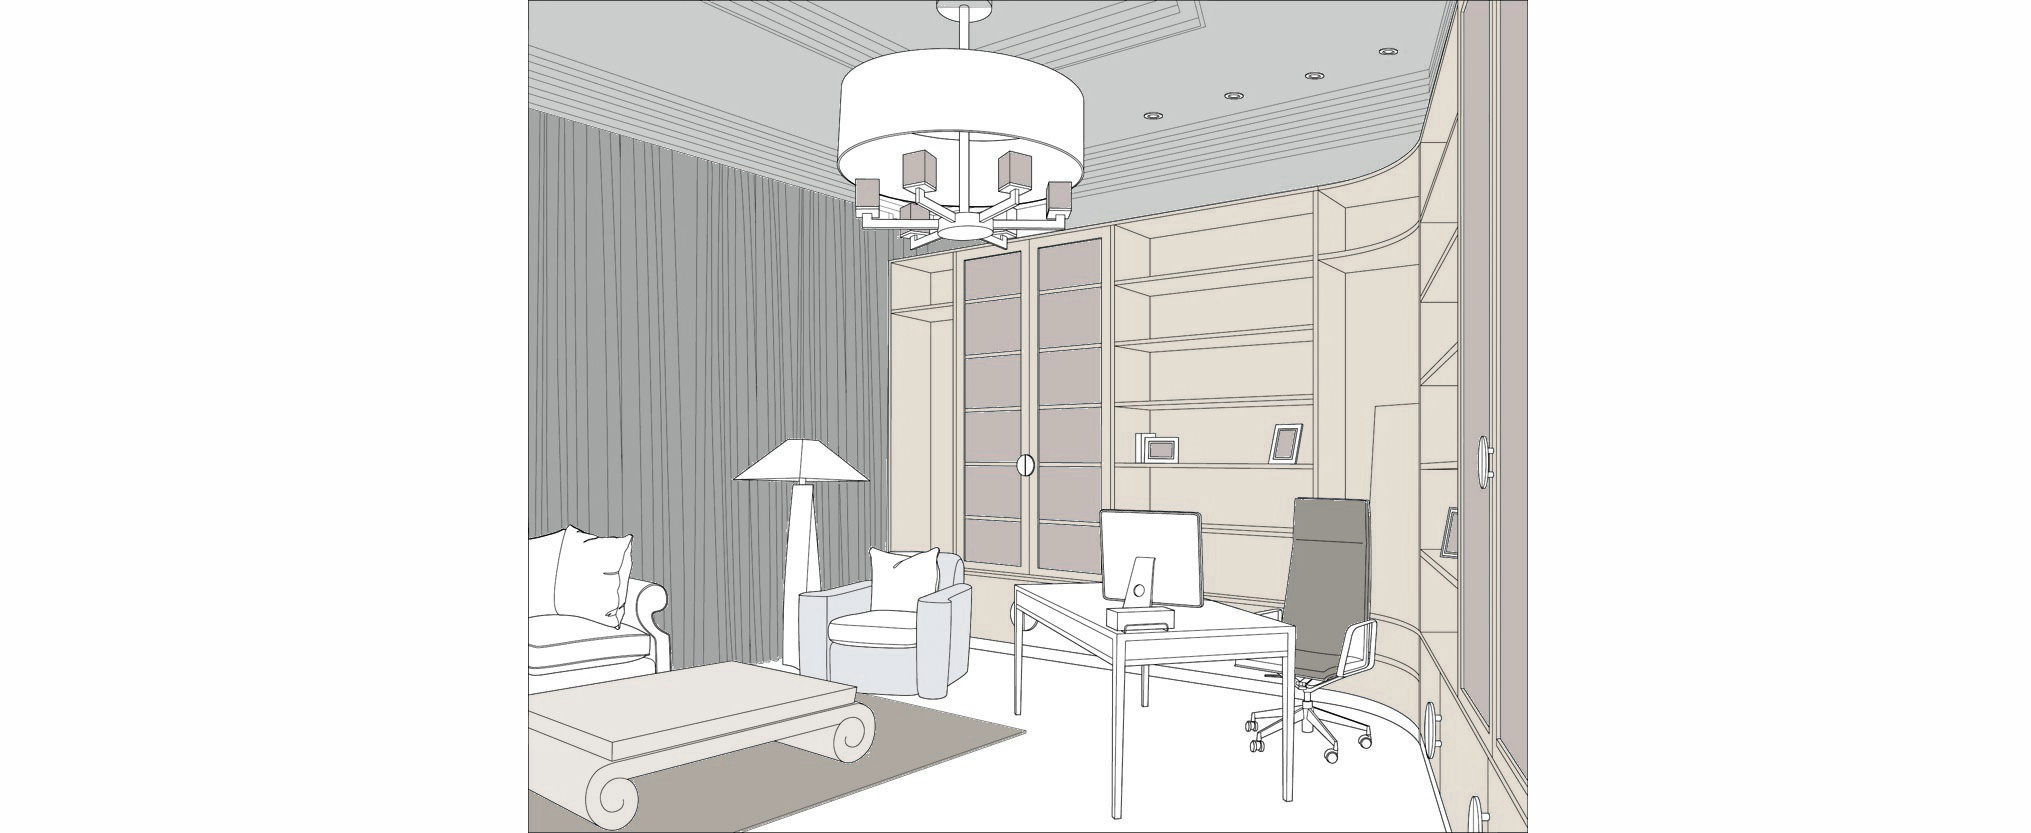
\includegraphics[width=\linewidth,keepaspectratio]{data/chapter-4/温柔.jpg}
\caption{输入“我想要温柔的柔和的感觉”}
\label{figure:温柔}
\end{figure}

输入“温柔的女性化的感觉”,作为人类的理解,这句话与上一句话的区别为,上一句话主要是“温柔/柔和”,这句话不仅强调“温柔”还强调“女性化”。输入“温柔的女性”,相当于对系统提出了两个要求,要求输出的结果既符合“温柔”又符合“女性”,得到的前20个艺术品为:

\footnotesize
“ 2009年作 温柔的坚持 布面 油画 ”;
“ 2009年作 你的温柔 布面 油画 ”;
“ 新女性 布面 油画 ”;
“ 新女性 布面 油画 ”;
“ 1993年作 温柔的光 布面 油画 ”;
“ 1997年作 温柔的风 布面 油画 ”;
“ 2007年作 下午温柔的阳光 布面油画 ”;
“ 2003年作 温柔的光 布面 油彩 ”;
“ 2003年作 温柔的光 布面油彩 ”;
“ 1989年作 温柔的音乐 油彩画布 镜框 ”;
“ 2006年作 新女性 布面油画 ”;
“ 2003年作 新女性 布面油画 ”;
“ 2003年作 当代女性 布面 油画 ”;
“ 1997年作 温柔的沉思 油彩 画布 ”;
“ 2002年作 新女性 布面油画 ”;
“ 2011年作 戴银饰的苗族女人 布面 油画 ”;
“ 2006年作 现代女性 油画 画布 ”;
“ 2007年作 美丽上海—她们的眼睛 布面 油画 ”;
“ 2010年作 优雅的女孩 布面 油画 ”;
“ 2013年作 优雅女人 布面油画 ”;

\normalsize
可以看到搜索结果其实分为靠近“温柔”的和靠近“女性”的,在“温柔”和“女性”结合的程度上显得不是很好,这样的结果收到数据库的限制,因为数据库中艺术品的文本包括“温柔”和“女性”两个含义的(并非必须这两个词)不常见。这是这个系统的一个限制,即数据库中的艺术品不能囊括所有的感受,并且即使艺术品中包含的信息和感受很多,艺术品文本包含的信息一定比艺术品本身少,艺术品文本描述的并不一定是艺术品的色彩风格。解决这个问题采用了交互设计的办法,即搜索最为匹配的前10个结果,对其中随机的一个提取颜色产生色彩方案。这样用户可以通过不改变输入文本,再次搜索,系统就会另外随机选择一件,直到用户得到满意的方案;用户也可以手动打开10个色彩方案手动选择。

对于配色方案我的期望是,比上图有更多的女性特质的方案,也许整体是偏粉红色或有其他符合女性特征的特点。而系统运行的结果如图~\ref{figure:温柔女},图~\ref{figure:温柔女2},是符合预期的。

\begin{figure}[!htbp]
\centering
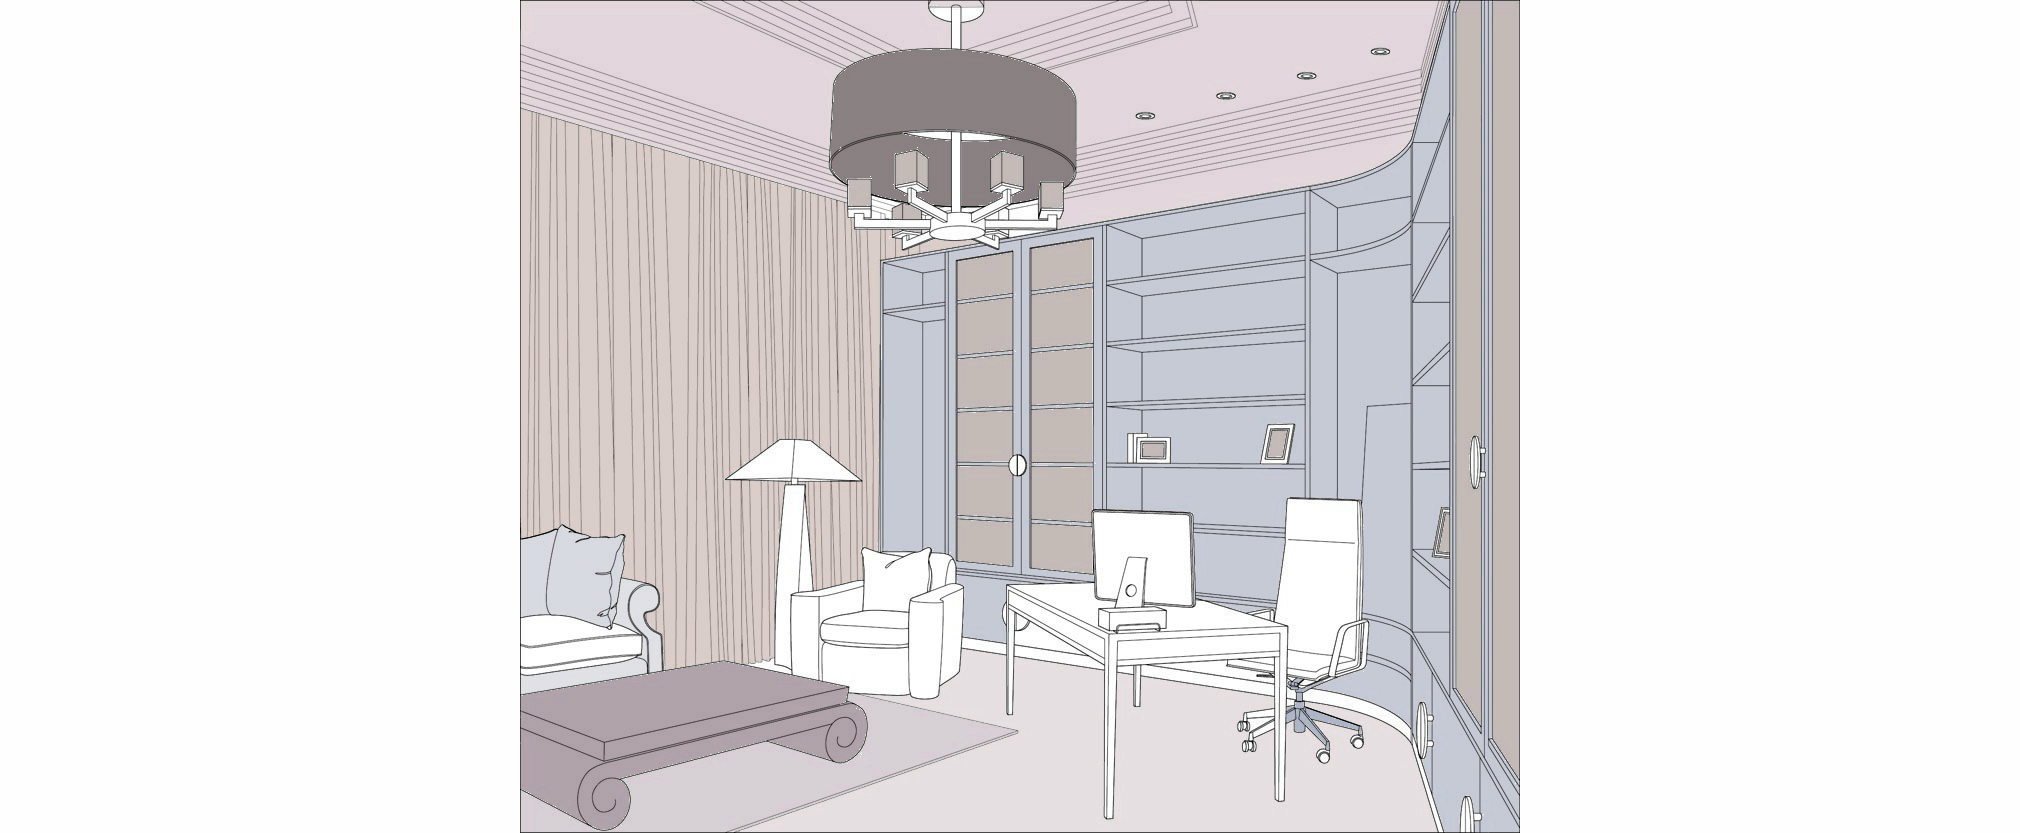
\includegraphics[width=\linewidth,keepaspectratio]{data/chapter-4/温柔女性.jpg}
\caption{输入“温柔的女性化的感觉”}
\label{figure:温柔女}
\end{figure}

\begin{figure}[!htbp]
\centering
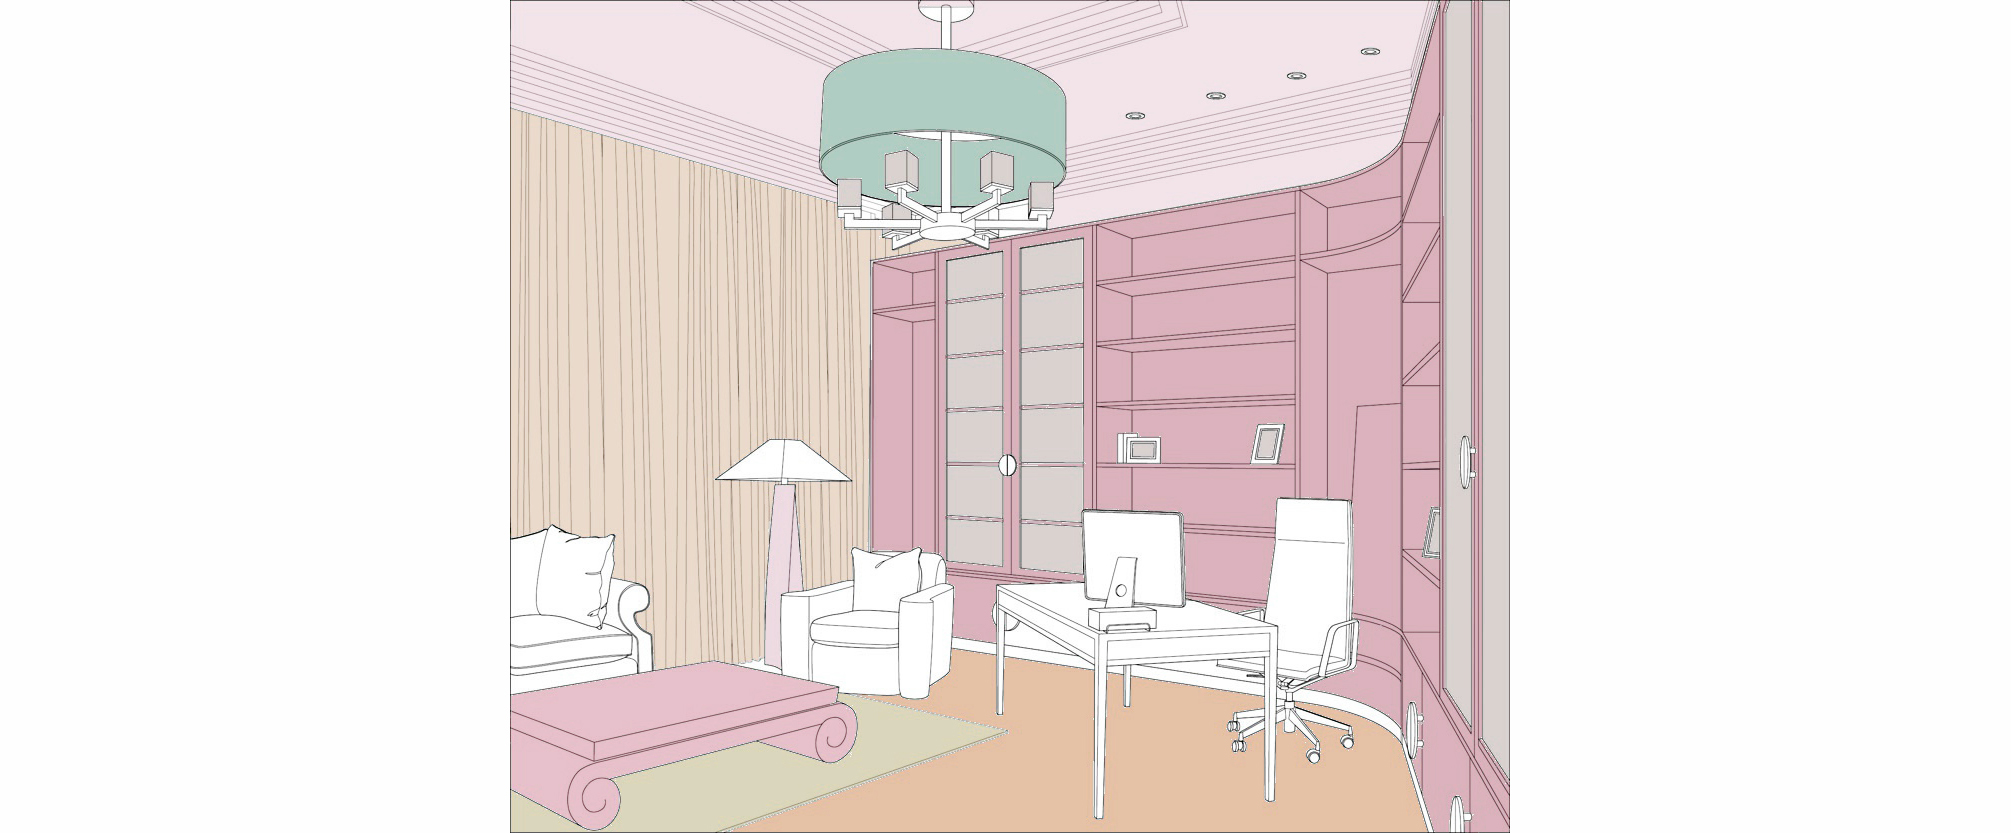
\includegraphics[width=\linewidth,keepaspectratio]{data/chapter-4/温柔女性2.jpg}
\caption{输入“温柔的女性化的感觉”}
\label{figure:温柔女2}
\end{figure}

那么如果输入“冷静的男性”。得到的结果是让人不满意的:

\footnotesize“ 新女性 布面 油画 ”;
“ 新女性 布面 油画 ”;
“ 2004年作 冷静 油彩 画布 ”;
“ 喻红在日常存在中寻找到一种诗意…… ”;
“ 2006年作 新女性 布面油画 ”;
“ 陈擎耀历年来的数字合成影像作品……”;
“ 我历年来的数字合成影像作品,皆……”;
“ 刘海粟是要强的人,有强烈的自我…… ”;
“ 1989年北京的现代艺术大展标志……”;
“ 刘海粟这个时期的作品有一种较……”;
“ 受马蒂斯的影响,闫平的画面中,表……”;
“ 2011年作 戴银饰的苗族女人 布面 油画 ”;
“ 不过站在美术史的角度上来看,从……”;
“ 居于大地的当代生存者正在描摹……”;
“ 2006年作 现代女性 油画 画布 ”;
“ 最显著的是911事件后,城市、霸权……”;
“ 《男男女女》创作于2006年,是刘……”;
“ 2003年作 当代女性 布面 油画 ”;
“ 2003年作 新女性 布面油画 ”;
“ 1999年作 理智与情感 油画 画布 ”;

\normalsize
在这里就发生了一个问题,想要男性化的风格得到的搜索结果全是女性。这是由于word embedding的词向量本身的性质。由于词向量基于上下文预测,所以最为相似的单词并非语义上最相似,而是用法上最相似的单词,比如“男性”和“女性”往往用在相同的上下文环境中,而“男性”和“男人”相对用在相同上下文环境中的程度更小一些。如果我们适应一下这个系统,输入“冷静的男人”那么就会得到这样的搜索结果:

\footnotesize
“ 2004年作 冷静 油彩 画布 ”;
“ 1995年作 大眼睛男人 布面 油画 ”;
“ 2011年作 戴银饰的苗族女人 布面 油画 ”;
“ 2007年作 红色男人 布面油画 ”;
“ 2006年作 男人像 油画 ”;
“ 清 男人像 纸本油画 ”;
“ 男人像 油画 画布 ”;
“ 男人像 油画 画布 ”;
“ 2008年作 男人 布面 油画 ”;
“ 两个男人 纸本 油画 ”;
“ 2005年作 男人肖像 布面油画 ”;
“ 男人的故事 ”;
“ 男人 布面 油画 ”;
“ 男人 布面 油画 ”;
“ 2007年作 红色男人 油彩 布面 ”;
“ 1999年作 男人与马 布面 油画 ”;
“ 喻红在日常存在中寻找到一种诗意。她……”;
“ 1997年作 同志系列:男人 布面 油画 ”;
“ 2006年作 红色男人像 油彩 画布 ”;
“ 2001年作 男人·女人 布面 油画 ”;
\normalsize

如图~\ref{figure:冷静的男人},比起“温柔”来看的确显得更加沉稳厚重。

\begin{figure}[!htbp]
\centering
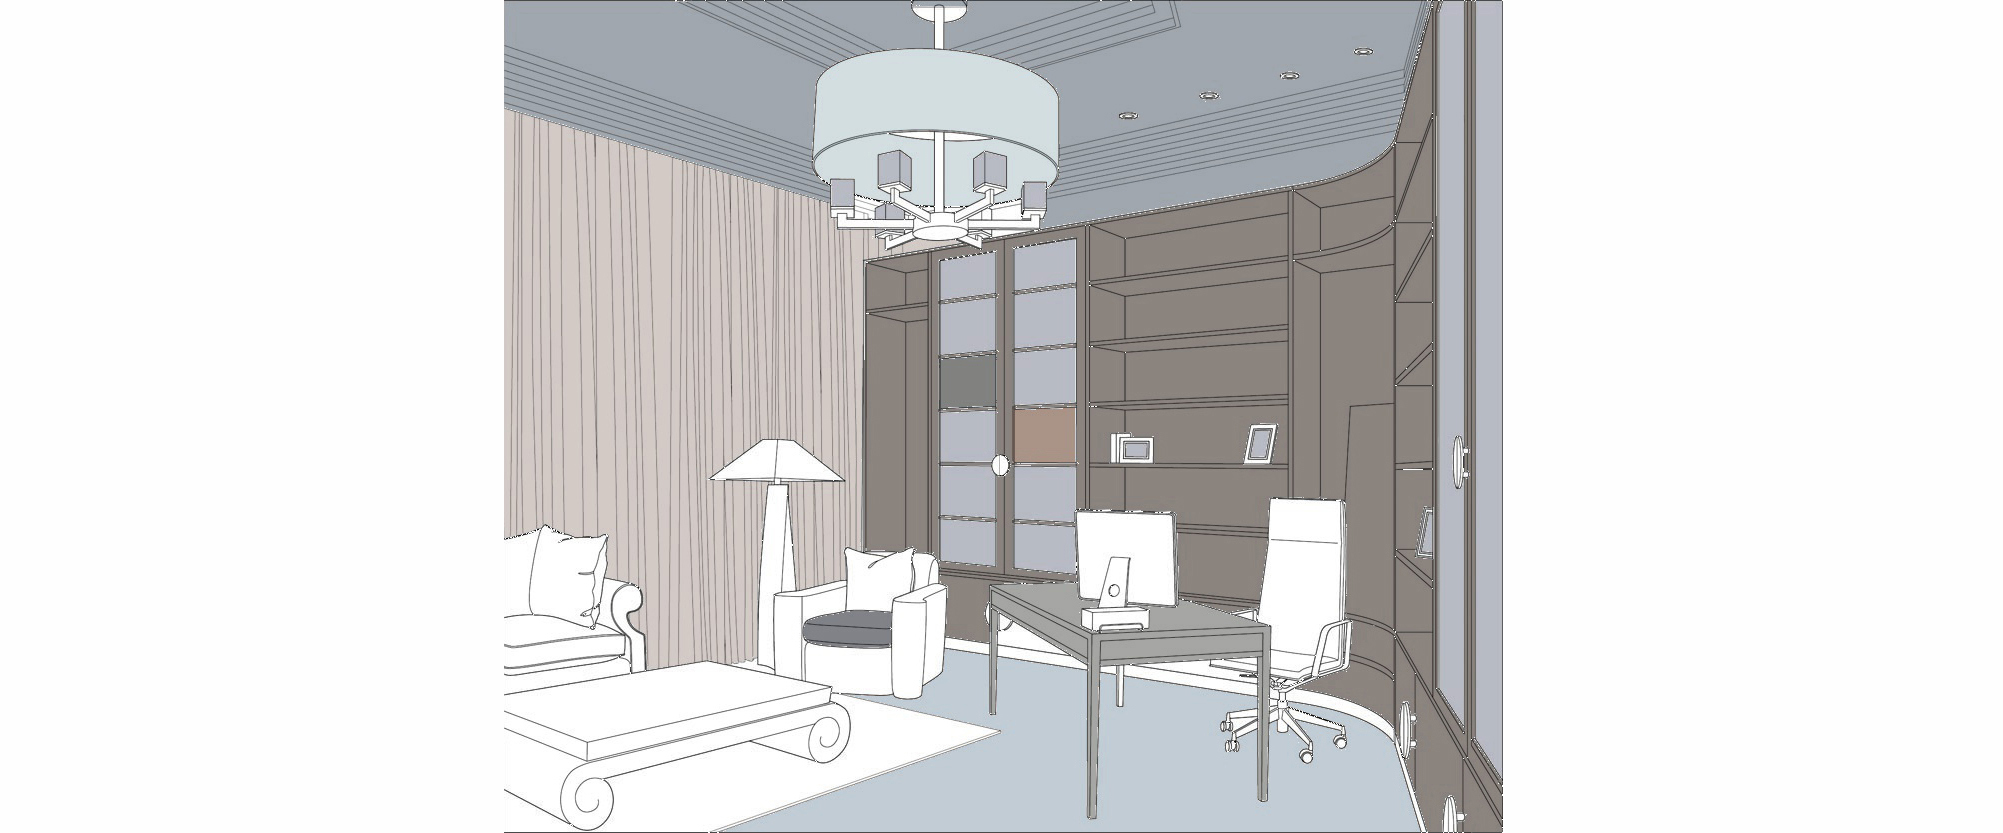
\includegraphics[width=\linewidth,keepaspectratio]{data/chapter-4/冷静的男性}
\caption{输入“冷静的男人”}
\label{figure:冷静的男人}
\end{figure}

输入“快乐的儿童”,输入“快乐的儿童”搜到的艺术品有:

\footnotesize
“ 1997年作 快乐的儿童 第9号 油画 画布 ”;
“ 2013年作 快乐的孩子们 布面油画 ”;
“ 新中国的儿童 (一张) 纸本 ”;
“ 儿童 布面油画 ”;
“ 儿童 油画 ”;
“ 2004年作 儿童时代 油画画布 ”;
“ 快乐1 油画 ”;
“ 1997年作 为小孩快乐 油画画布 ”;
“ 2001年作 快乐世界 布面油画 ”;
“ 少女与儿童 布面 油画 ”;
“ 2005年作 快乐在一起,2号 油画画布 ”;
“ 快乐的童年 布面油画 ”;
“ 1999年作 快乐的红色 油画 画布 ”;
“ 1992年作 快乐 油画画布 ”;
“ 游戏的儿童 布面油画 ”;
“ 快乐的童年 油画画布 ”;
“ 威尼斯的快乐 ”;
“ 2002年作 游戏的儿童9号 油画画布 ”;
“ 2002年作 游戏的儿童8号 油画画布 ”;
“ 2005年作 快乐组合 布面油画 ”。

\normalsize
显示程序完全可以抽象出“儿童”和“小孩”、“孩子”的相似性。得到的图~\ref{figure:儿童2}的色彩方案,虽然使用的效果图线稿是一个书房,但是也能看出符合方案儿童房的配色。

\begin{figure}[!htbp]
\centering
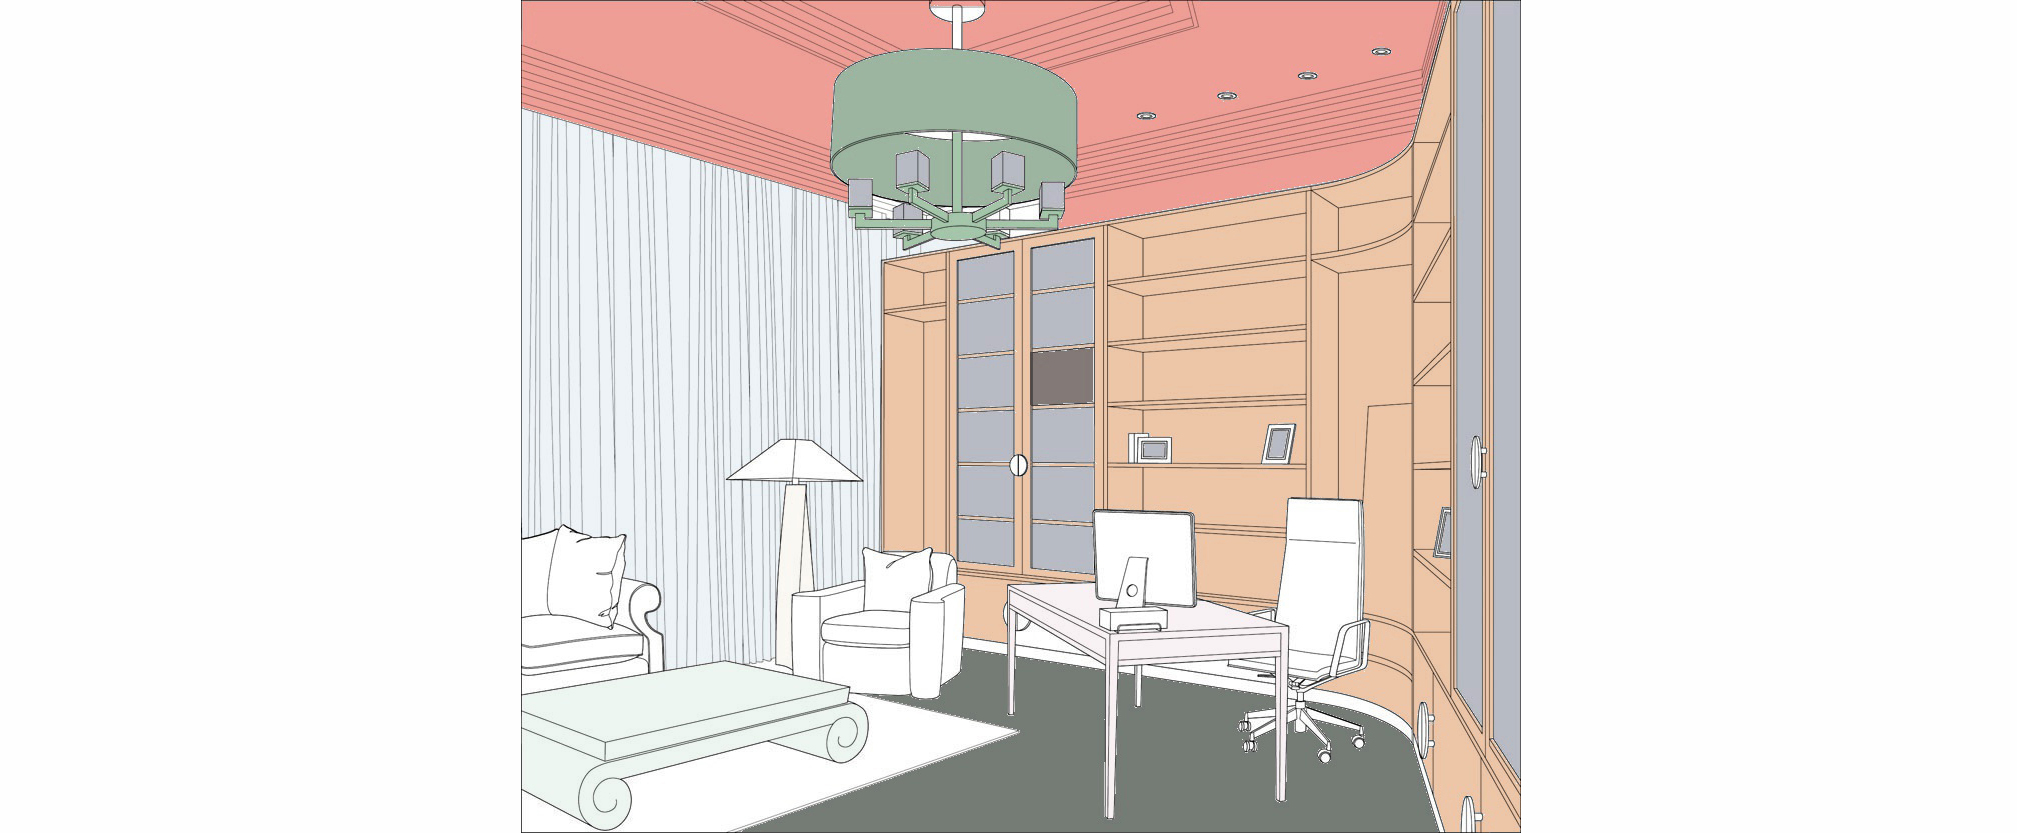
\includegraphics[width=\linewidth,keepaspectratio]{data/chapter-4/快乐儿童2.jpg}
\caption{输入“快乐的儿童”}
\label{figure:儿童2}
\end{figure}

\begin{figure}[!htbp]
\centering
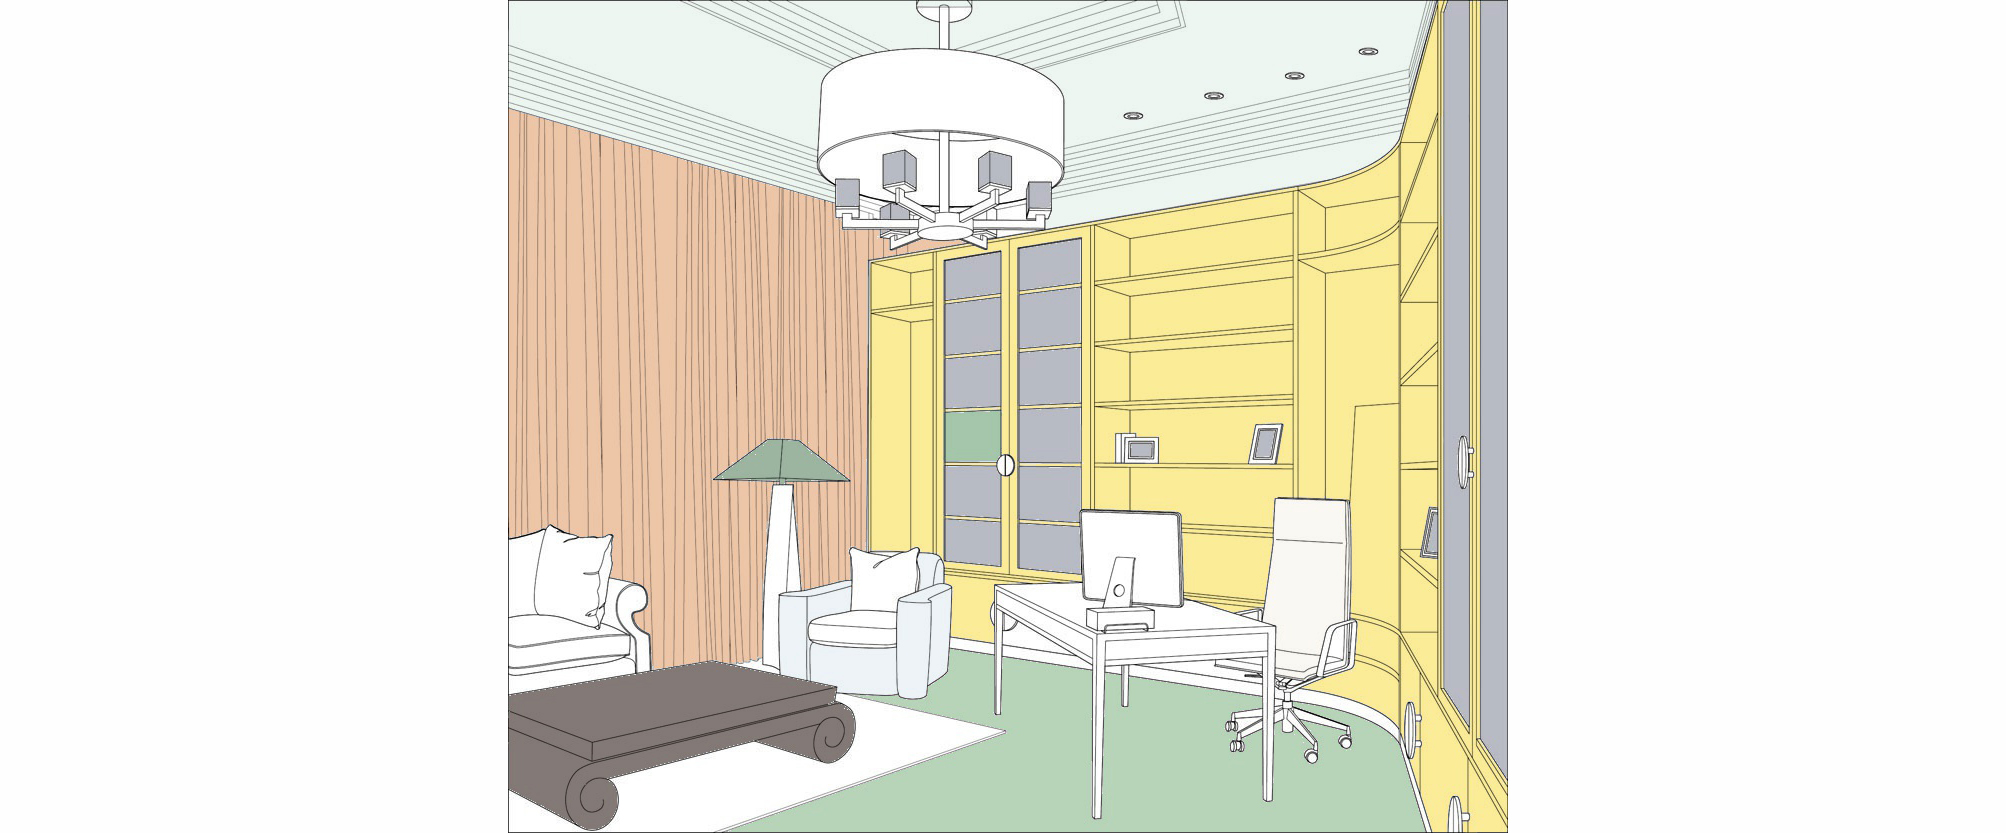
\includegraphics[width=\linewidth,keepaspectratio]{data/chapter-4/快乐儿童3.jpg}
\caption{输入“快乐的儿童”}
\label{figure:儿童2}
\end{figure}



\section{效果图类型的测试案例}

本系统的色彩方案可以用于室内设计、服装设计、产品设计、平面设计、交互视觉设计等。但是上色预览的算法并不适用于每种工作。系统准备了室内设计,服装设计各1套效果图线稿预览,之测试发现,如图~\ref{figure:温柔_IandF},对于上色区域占图片比例较小并且色彩有限的服装、产品效果图本系统也可以使用,但系统效果更适合室内设计效果图。

\begin{figure}[!htbp]
\centering
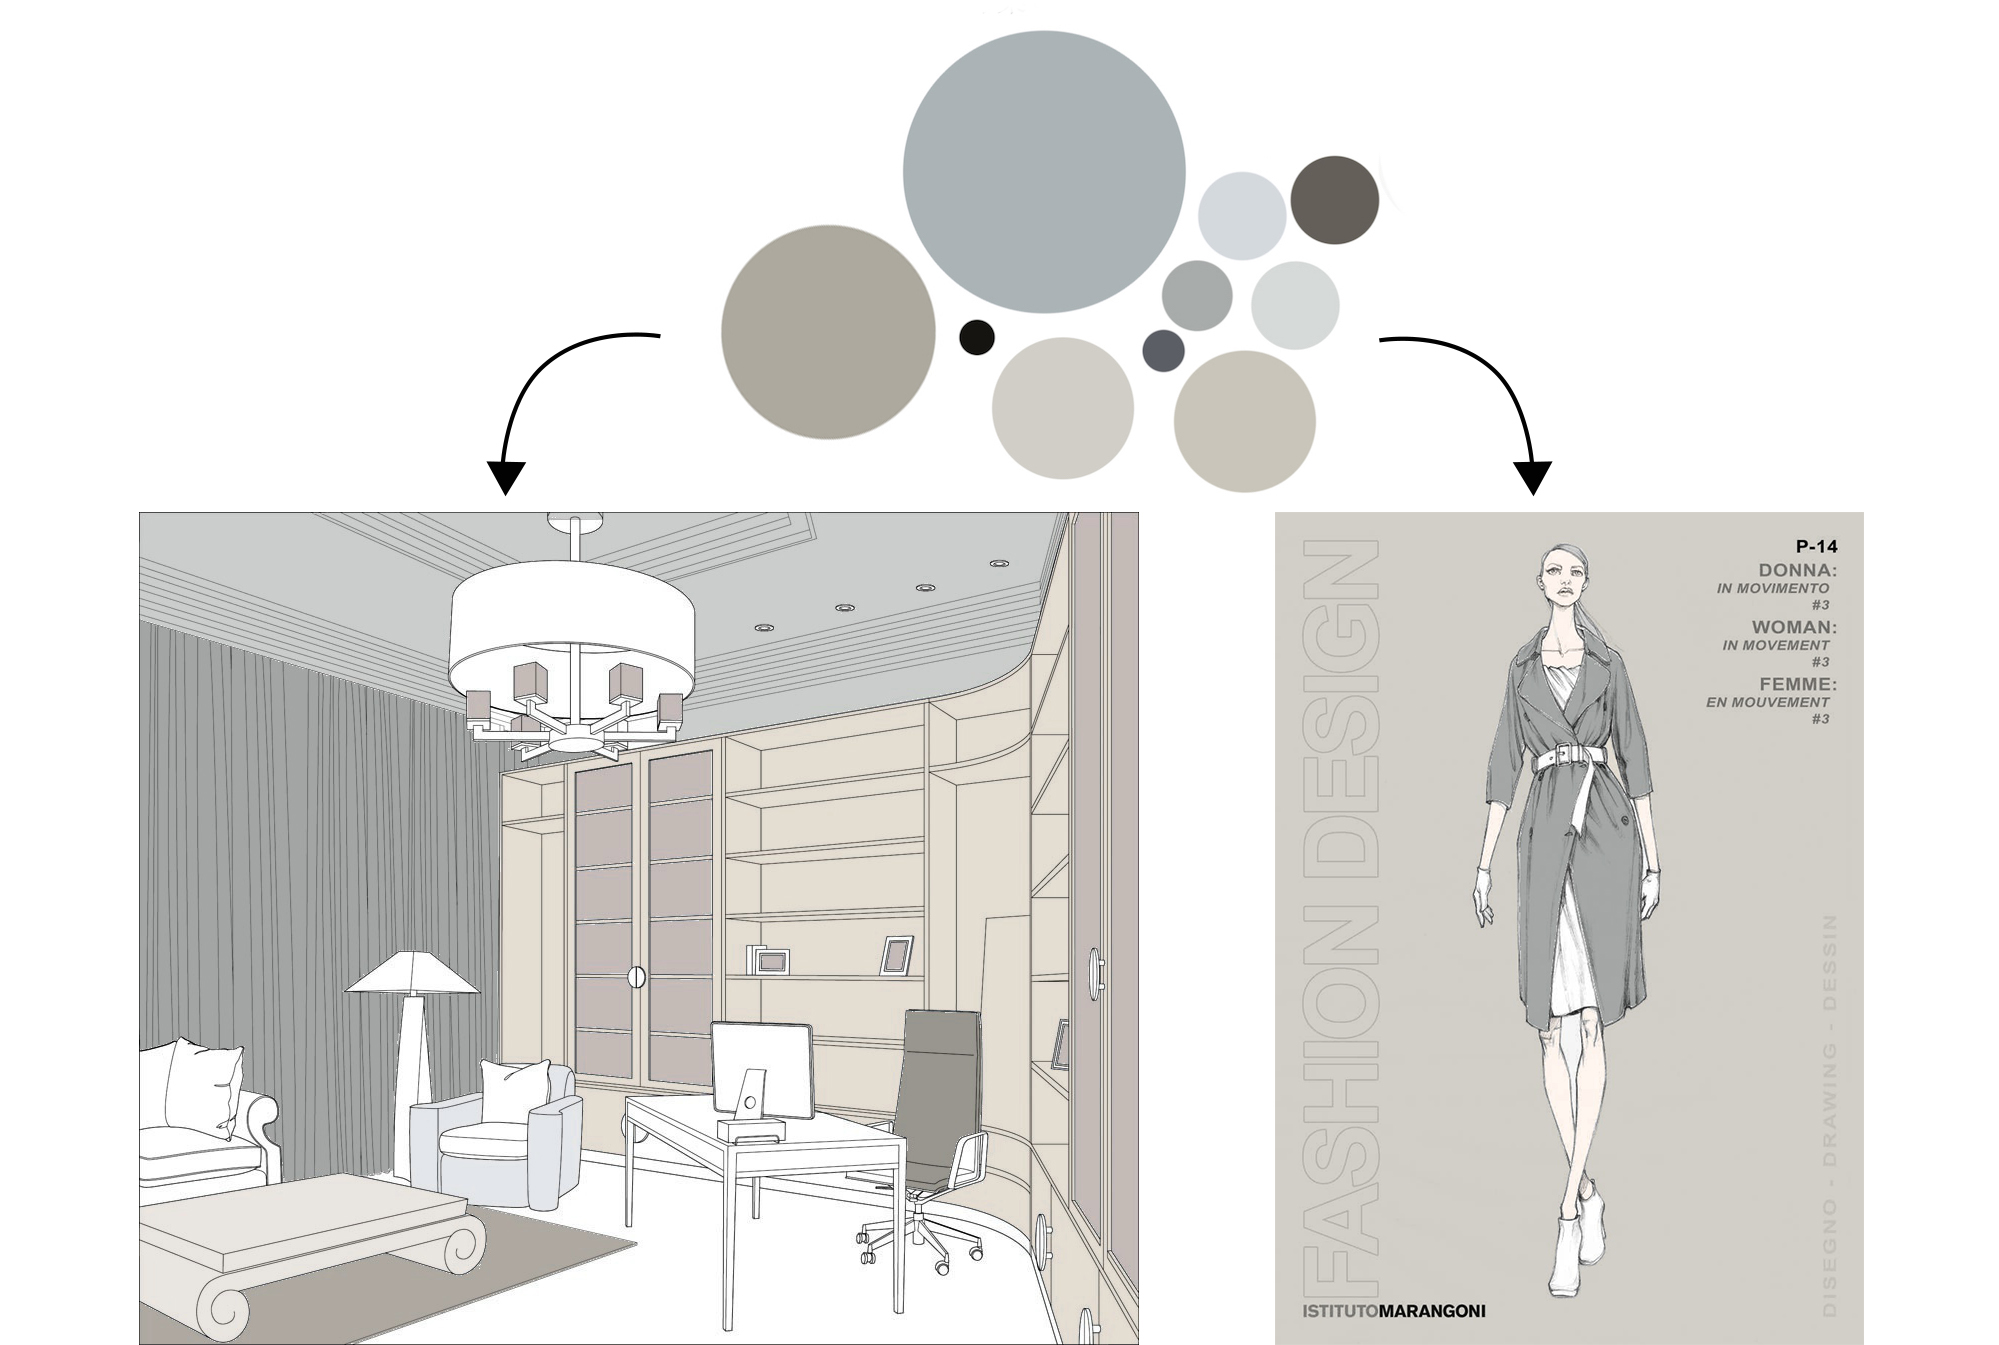
\includegraphics[width=\linewidth,keepaspectratio]{data/chapter-4/温柔_IandF.jpg}
\caption{色彩方案:“温柔”对室内设计和服装设计效果图的预览}
\label{figure:温柔_IandF}
\end{figure}

配色方案对于服装设计是适用的,然而由于服装设计效果图有一些特点,首先服饰在整个图片上的面积较小,填充算法的种子点行走到服装上到几率较小,如果是有花纹的服装,花纹的色彩连续性无法保证,小的配饰更难以填充,所以本系统的上色算法更适合室内设计。

对于其他的效果图,可以使用具体匹配的上色方式。对于产品设计效果图,每个产品上的出现颜色不多,可能有成套的不同颜色的产品,更适合简单的标注上色预览。而对于网站视觉设计等,网页的框架往往预先设定比例和模式,使用堆栈的方式上色是非常适合的,在很多的情况下网站设计适用矢量图片,可以直接标注色彩上色。综上,上色方式并不适用某些效果图,但配色方案对于产品设计、网页设计都是适用的,

\section{本章小结}

经过输入语句测试案例,本系统可以对语义精确的响应。对于“冷静的男性化的”房间、“温柔的女性化的”房间、“快乐的儿童的”房间,配色有明显的差别,符合人类的心理预期。而对于“温柔的”和“温柔的女性化的”,这样信息叠加的语句也有相似而差异的配色方案结果。

对于文本不同而意义相同的语义延伸词语,本系统的word embeding模型能够实现同义匹配,并且将其排列在文本完全相同的情况之后搜索到。对于不含有信息的干扰语句,本系统的word embeding模型能够实现信息提取,和不含有干扰语句的情况下得到的结果差别很小。对于含有并列信息的输入语句,搜索的结果受到艺术品数据库的限制,不一定存在完全符合所有并列信息的艺术品文本,所以搜索到的文本结果分为偏向各信息的内容,使用交互的方式来解决这各限制带来的偏差。

对于效果图的类型,本系统的色彩可以用于室内设计、服装设计、产品设计、平面设计、交互视觉设计等。但是上色预览的算法并不适用于每种工作,本系统的上色算法更适合室内设计效果图。对于产品设计、网页设计、服装设计等工作,可以使用各自匹配的上色预览算法。








\backmatter
\bibliography{reference_data_base/references_1.bib}
% \nocite{*} % to show the entire references, annotate it if need.
% !Mode:: "TeX:UTF-8"
% !TEX root = ..\main.tex
\chapter{致谢}
岁月如梭,转眼间,三年的研究生求学生活即将结束,站在毕业的门槛上,回首往昔,奋斗和辛劳成为丝丝的记忆,甜美与欢笑也都尘埃落定。浙江大学以其优良的学习风气、严谨的科研氛围教我求学,以其博大包容的情怀胸襟、浪漫充实的校园生活育我成人。值此毕业论文完成之际,我谨向所有关心、爱护、帮助我的人们表示最诚挚的感谢与最美好的祝愿。

本论文是在导师孙守迁教授的悉心指导之下完成的。三年来,导师渊博的专业知识,严谨的治学态度,精益求精的工作作风,诲人不倦的高尚师德,朴实无华、平易近人的人格魅力对我影响深远。导师不仅授我以文,而且教我做人,虽历时三载,却赋予我终生受益无穷之道。本论文从选题到完成,几易其稿,每一步都是在导师的指导下完成的,倾注了导师大量的心血,在此我向我的导师孙守迁教授表示深切的谢意与祝福!

本论文的完成也离不开其他各位老师、同学和朋友的关心与帮助。在此也要感谢张克俊、汤永川等各位老师在论文开题、初稿、预答辩期间所提出的宝贵意见,感谢创新设计课题组为本论文提供的数据和建议,还要感谢同门的师兄师妹们,在科研过程中给我以许多鼓励和帮助。回想整个论文的写作过程,虽有不易,却让我除却浮躁,经历了思考和启示,因此倍感珍惜。

还要感谢父母在我求学生涯中给与我无微不至的关怀和照顾,一如既往地支持我、鼓励我。最后要感谢我的男友,在学习期间给我的支持和帮助,也在生活上给予我包容与鼓励。

\vspace{2cm}
\hfill
\begin{minipage}{14em}
\begin{center}
于求是园\quad 2018年4月16日\\
胡迪
\end{center}
\end{minipage}

\appendix
\chapter{附录:实验结果}
\section{文本搜索结果}
\footnotesize
\subsection{输入:温柔}
“ 2009年作 你的温柔 布面 油画 ”;

“ 2009年作 温柔的坚持 布面 油画 ”;

“ 1997年作 温柔的风 布面 油画 ”;

“ 1993年作 温柔的光 布面 油画 ”;

“ 2007年作 下午温柔的阳光 布面油画 ”;

“ 2003年作 温柔的光 布面油彩 ”;

“ 2003年作 温柔的光 布面 油彩 ”;

“ 1989年作 温柔的音乐 油彩画布 镜框 ”;

“ 1997年作 温柔的沉思 油彩 画布 ”;

“ 1992年作 温柔情人 压克力纸本 ”;

“ 1992年作 温柔情人 压克力 纸本 ”;

“ 2013年作 夜色温柔 布面油画 ”;

“ 2010年作 夜色温柔 布面 油画 ”;

“ 温柔地杀我 油画 画布 ”;

“ 2004年作 温柔地杀我 版画 ”;

“ 2002年作 温柔地杀我 布面 油画 ”;

“ 2010年作 优雅的女孩 布面 油画 ”;

“ 2009年作 你的柔情 布面 油彩 ”;

“ 灿烂的朝阳照在秋日收获的黄土高原上,辛劳纯朴的陕北女孩儿用心爱的笛子吹起悠扬的音乐。这笛声飘荡在静穆的村庄上空,诉说着古老而遥远的传说。陕北女孩儿的柔情与这秋日辉煌形成鲜明的对比,从而更加突出了女孩儿的纯情和对未来人生的美好憧憬。 ”;

“ 2009年作 你的柔情 布面 油画 ”;

\subsection{输入:我想要温柔的柔和的感觉}
“ 第二年,我去了北京,在那里整整住了一个冬天,窗外飘着大雪。味道不佳的室内,暖烘烘的,在这里我画了一批工厂和管道与植物交织的作品,牧歌式的景观被分裂和忧郁的超现实图式所代替,这一个是著名的85美术思潮涌动的时候,超现实主义的大师达利、契里柯的追随者在中国的这页美术史中大放异彩,与注重哲学思考和文化批判的理性思考不同的是:我是由纯粹个人经历和感觉自然的过渡到超现实语境的。我喜欢已沉迷于文化风暴而心灵脆弱的内心为表达主题:因为想太多而行太少,因为书读得过多而体会过深,人格失调、精神分裂、失意、堕落或彷徨接踵而来。《离开和留驻在最后一块草地上的两个人》、《屋外的马窥视的她和被他端视的我们》、《最后的花园》、《听见毕加索马叫的隐者和鸟》、《春天唤醒冬眠者》是这时的作品。虚幻失真的田园憧憬,平庸沉闷的现实生活、虚假的文化表象与躁动的思潮迷雾之中,是绘画使我解放出来,为我展开一个新的景界。一切静止不动,一成不变的东西都开始颤栗了。不只是被人赋诗的星星、月亮、树林、花草,甚至一团发电厂的烟灰,一张被风吹到街角的报纸,一块不知所以然被蚂蚁从草丛里咬出的树皮,一座锈蚀的、停摆的座钟……所有的一切都显露给我一张自己的脸,它内在的生命,这些沉默的心灵。经常无声胜有声,无论静或动的点或线对我都是这般生动,这就足够使我投入整个生命感觉去体会艺术的可能性和它的生命。自然地将自己的梦境表现在画布上,并且化痛苦为诙谐,化诙谐为抒情,像鱼一样,流连在自己的幻想中,那时,对我而言,绘画几乎是人与动植物和工厂之间的一种混合体。 ”;

“ 受马蒂斯的影响,闫平的画面中,表达观念时,依靠的是色彩而不再是传统写实中的光与影,体现光线的感觉是通过色彩的对比与排列来表现的,而不仅仅是描绘形体。从画面的色彩来看,戏剧的服饰能够充分彰显出色彩的艳丽,画乍看张扬,细看则处处小心,如同喜剧演员台上台下判若两人,色彩的叙述有一定的私密性能让她尽情地表达内心世界。颜色是外在的,而内心要表达的情绪置于其中则具有保护性、自由性和私密性。在此画中,我们不仅可以看到有后印象派的影响,还能看到对中国传统艺术文化的传承,画面中融会贯通了西方的理性秩序和中国的意向表现,在理好的色系画面上,加上特立独行的焦墨,恰到好处。纳比派的主观表现给了闫平以启迪,加强了用色的浓度和画面的装饰性处理,使色彩相互交织,对比与协调并存。画面中,闫平大胆运用强有力的笔触进行塑造,由薄到厚,由于作品中用笔交错相叠,产生了一些犹如砾石般的肌理,使得画面的表现更加丰富。从画面的构图来看,她把握大局,对于画面的四边四角和主体物之间的关系的处理非常考究。这里面包括:画面的分割,每一个线条的长短,每一个方圆的比较,画面中疏密的安排以及造型方式的扩展等等。 ”;

“ 杨飞云的艺术真正打动人的,与其说是他通过学习西方古典艺术的绘画形态而将古典主义移植到我们这块土地,不如说是他将古典的精神通过他独特的灵魂体认而呈现在我们面前。为一个人,他有幸感领到永恒的生命奥秘,作为一个画家,他有幸以第二双眼睛看到了世界的荣光之美,正像他所说的:“感谢造物主,给我们提供了如此缤纷煊丽深沉广博的自然世界,内里深藏井然有序的规律、外有瞬息万变的勃勃生机,丰丰满满的不缺少什么,供我们探求和寻找想欲的一切。” ”;

“ 这种自觉的留白和色彩的简括处理是一种新的绘画性格,它是油画形态发生改变的重要端倪,它必定被后人发现和珍视,这种新的端倪预示了在西方光色和结构两大语言谱系之外,油画语言开放的另一通道。刘海粟通过书写与塑造的重新匹配,油画被另一种民族智慧所把握,补充和开放了油画这一古老艺术样式的“音域”,这就是贡献,对绘画表达和视觉审美经验的双重贡献。这是一个东方少年天才自悟自通的发明。《圣扬乔而夫飞瀑》无论是作品形态和完整度还是语言的成熟度,都已经达到那个时代的最高水平。在一定意义上,这是被逼迫和放纵出来的才情,任性和要强的情绪通过书写的动态挥策而出,如瀑布流泉一样奔涌、流淌出来,笔下的物象已经不是静态的客观物象,更像是一个充满热情和煽动感的视觉宣言,预示着观看习惯和表现陈习的巨变。尽管这个巨变被中断、覆盖,在历史视野中消逝了近八十载,今天让我们看见它,就如蓦然看见了旷代知音,本能般萌生一种把臂欲言的冲动。 ”;

“ 居于大地的当代生存者正在描摹一幅高度机器化的是日常生活图景,已经取得的物质成果并没使人们获得更多的幸福和精神自由。人们陷身于自己的创造物中并被其所奴役。丁方为我们提供了新的视觉经验:广阔空无的黑暗,在我们的体内发出回声,一个恍惚而苍白的的飞翔人形在浊浪翻滚的昏暗中挣扎飘荡,所有鲜活的生命都被这一片混沌无情遮没着,即沉重工业的压迫之力逼使人们集结突围的勇气和力量,抵抗和承担由恐惧所预感到的否定性(《我逃向何方?》);一条没有来处和去处的褐色河流挟裹着颓废的建筑残体和无知无觉的肉身,面对这种毫无反抗的挣扎努力的自溺情形,绝望感几乎要漫过我们的头顶(《罪灵们》)。此时,坚信者的呼告之身形迎面而来;精砺的铅色背景上,一个巨大的鸟形幻像,犹如折翼的天使,正飞向黄昏中模糊的地平线,羽翅上青洌的光芒耀亮即将陷入昏暗的荒野(《折羽的天使》、《请退让吧,忧郁的阴影》)。这些画幅突破了艺术的唯美法则的宥限而均突出了其思想的锐利;神圣关怀并没有抛离人,只要人愿意,就在此时此刻,他会来与我们相遇,以其苦痛搀扶人的苦痛。 光影。古典的光影效果重新返回丁方的画面,光对画面的统领使其显示出蕴于悲剧深处的庄严性。丁方画面中精神性光影的设置,作为神圣俯临此世的标志,它显征着叹息、救扶、怜悯、启明、爱等精神内涵,它不是来自熟常的经验世界,它温抚着画面肌理的紧张断裂,呼应着上升的精神,漫渗到流幻的色彩深处,洞开灵魂的奥秘。它在显示生命的悲剧况味的同时,“给予灵魂以永恒的召唤”。在这种精神之光的携领下,丁方的画语世界凸现出几个非常重要的意象造型:以黄土高原、荒野自然为原型的大地意象。作为众生灵终其一生、存活于其上的大地,其深邃、厚重的自然存在形态在丁方的画面中取得超拔于日常感觉经验的独语性:奔泻而下的色流形成大地强烈的动势,坚岩般的肌理沉凝滞重,深含着忍耐、重负和强劲的生存精神。 ”;

“ 20世纪80年代以来,他从写实到表现,走上了一条更为宽阔的道路。他的表现不是苦涩的,而是歌吟式的,也就是抒情的,这是他的人生观与世界观的体现。他总是希望现实与理想接近一些,试图用自然生命的热烈与蓬郁气象缓解现实生活的苦恼与矛盾,用美好的向往引领人们的精神世界。他的艺术风格兼蓄了许多属于“成熟”境界的因素,例如文艺复兴诸家晚年作品那种浑然的氛境、印象派各位到后来信笔流淌出来的华彩、属于表现主义语言根本的那种急疾而鲜活的“手气”。他也将中国传统美学中崇尚“骨气”,注意综合,以阐发人与自然亲和关系等优点融化到自己的作品之中,由此不断朝向表达更自由、笔力更老辣、抒发更从容的境界迈进。 ”;

“ 那年冬天,我经常去美术馆看一个接一个的展览,劳申伯的大型展给我不同与往的震撼。它虽不像其它我所看到的《韩默藏画展》、《法国250年藏画》、《德国表现主义画展》、赵无极、戈雅、柯尔韦尔个展等古典和现代主义那种对自我情节的顶礼膜拜具有令人驻足叹服,品评赏析的细节,但却使我第一次强烈地感受到当代艺术直接切入周遭生活的力量。这与我几年来接受的为艺术而艺术的教育很不相同,这也使我先前即已产生的对“纯美术”意义的质疑更得到证明。1986年朋友们同我一起发起和组织的《西南艺术群体》,使我更直接投身于“新潮美术”的潮流中。我们彻夜地谈论种种宣言和观念,策划在昆明、上海、重庆和北京的展览,在各种报刊上撰写文章,对那些同样激动得面红耳赤的人解释何为“新具像”——那的确是一个冲动的年代,经历过八十年前期文化洗礼的人们,例如我本人,总是难以忘怀那些热闹的场面。虽然那时的文化存在诸多的夸张,自以为是和种种谬误,但是,那毕竟是一个在文化上有追求的年代。毛旭辉永远紧锁着眉头,在和平村的小屋中挤满了《他的红色体积》和其它许多的作品,他的东西令人压抑、难受。与此相反他却能写一手漂亮的激扬文字。潘德海总是结结巴巴地发明一些惊人的词汇,除了画《杂乱的、杂乱的》形象,还用泥巴做了一大堆黑不溜秋的怪物。张晓刚则一直有点善感和见异思迁;胃病住院就画些痛苦的痉挛不堪的《白色幽灵》;搬到桃花山又显得花花草草地吟诵《遗梦集》……今天,当年年轻气盛的他们都已一个个成为了不起的画家了。那个时候,我在医院里一面等待女儿的出生,一面写《自然意识略述》和《丛林猛兽》。在省图书馆的展览开始时,朋友们在请柬上写满了对未出生女儿的祝福……同当时的许多知识分子一样,我们怀有真实的人文主义理想,虽然今天我的同辈们大多数未必赞成那种理想,然而在情感上却仍又存在深深的怀念。 ”;

“ 1993年作 温柔的光 布面 油画 ”;

“ 2003年作 温柔的光 布面油彩 ”;

“ 2003年作 温柔的光 布面 油彩 ”;

“ 2007年作 下午温柔的阳光 布面油画 ”;

“ 1989年作 温柔的音乐 油彩画布 镜框 ”;

“ 刘海粟这个时期的作品有一种较劲和任性的情绪,与日本第一代“准印象派”艺术家的作品相比,他自觉的东方性格已经完整地呈现出来,甚至是近乎偏执的强调这种性格。他的写生作品与日本前辈画家黑田清辉和藤岛武二的相比,更具书写的自由和流畅感,情绪更为敏感、张扬,色彩更为刺激、强烈,他自觉的弱化了色层堆叠和塑造感,以柔性的笔调书写出阳刚的气质,他完成的语言难度是巨大的——以柔致刚,以简驭繁,以轻薄而致厚重。在他1930年代的代表作中,我们可以看到他明确而自觉的语言策略。一个优秀的艺术家,策略自觉、成熟的标志就是——他将那些难以结合的矛盾双方确立为自己的表现范畴,将相反者结成紧密的同一,这就是艺术命题的方向,天才往往就是在那些难以逾越鸿沟间自由腾挪的人。从文化背景上来看,刘海粟当年也是承受着双重的文化压力,反者道之动,最对立的矛盾双方往往是触发天才属性的直接动因,只有那些能主动挑战并立志于战胜这些截然对立矛盾的人,才可能创造出历史的奇迹——不可思议的难度是历史奇迹的前提!刘海粟之所以伟大,在于他克服甚至颠覆了中国传统文人的内向、惰性、柔美的审美趣味和文化性格,但又将文人细腻、敏感、神秘的趣味特征糅合进了全新的表现形式之中,结成了相反者之同一;同时,他颠覆了当时国内以及整个东方艺术领域对客观再现的迷恋——他在这两种主流美学趣味的压力之下寻求突围的通道,以非常态的学习方式和创作风格如一匹黑马腾空而起,成为时代的英雄。他1930年代创作颠峰的作品基本致力于转化后期印象派的语言和形态,具有超前的实验精神,比日本梅原隆三郎1930年代晚期的中国写生,更有一种从容的气度和灵敏的语言才华。 ”;

“ 1982年我毕业后被留校任教,浪漫的、不着边际的学生生活同平庸乏味的现实生活的差别很快显露出来,尽管此时我被周围的朋友们认为是个“幸运儿”——在毕业前我已是“美协会员”,作品也参加和发表在各种展览、杂志上,抽屉里藏满了入选、获奖证书和来自各地的初学者的来信。但是很快这种小小的满足感就消失的一干二净,首先是一度在全国独领风骚的四川油画,已失去其尖锐的社会抗争性,在受到普遍的赞誉和认同后,业已成为一种日益陈旧和庸俗的样式范本,从思想与风格都同此有距离的我的作品几乎没有起码的参展和发表机会。其次,作一个为人师表的教师的现实与我内心幻想的那种“波西米亚式”的艺术家生涯相去甚远,同时我居住、工作的美院四周重庆典型的旧工业景观使我倍感压抑。透过发电厂巨大的烟囱冒出的滚滚浓烟,阴霾的天空下,灰色的街道泥烂如河,排放废气的喧哗声有如雷鸣,夜空为之震颤——在蓝天和树阴下长大的我想躲避的就是这个世界!对付这种日子的最好办法是去一个防空洞里开设的小酒馆里喝酒,每天,从黄昏时分起我就开始酝酿情绪,等待那喝酒的时刻终于来临。小酒馆里坐满了疲惫的夜班的巡道工,兴高采烈的白日扛活的搬运工以及就着铁丁下酒的酒鬼和守在角落里的默默无语的失意者。我虽是他们中间的一员,却难以排解难言的孤独,在一次半醉半醒之间的日记中我问自己:“你同周围世界格格不入,你无法和他人苦乐与共,你感到自己和他们隔膜甚深,这时你该怎样生活?”有时,我也只好自我安慰:“我还是不断地听到一种责备,指责自己缺乏现实的感觉,我的确是不尊重现实,我认为,现实最不需要人们充分地去注意,人生活于现实中永远不可能满意,因为现实是一种偶然性,是生命的垃圾,对于这种可怜的现实,我们除了否定它之外,别无选择。” ”;

“ 具象和抽象迭合构成的"古典"作品,给人一种包容性的丰富特征,这也就使得解读杨飞云的作品并非那么简单,在他那里既有古典大师的决定性的影响,也不乏塞尚、马蒂斯等现代画家的印迹。不过,难能可贵的是,杨飞云艺术作品的多层性,并没有给人生硬组合之感,读他的作品犹如聆听一曲旋律美妙清纯的小提琴独奏,其境界有追随东方高山流水和西方天堂之音的韵味。 ”;

“ 他的深度绘画表现和塑造的是具有当下性的永恒图景,其重要特征展现为一种弥漫于画面中的重返生存大地的勇气与决心。在这块安置人但又不能使人安居的大地上,他感受到表面欢娱下的人的苦难与绝望,并在绝望的深处发现了与人类苦难同在的神圣。无形的灵魂世界运行于涌流的色群之中,将要急掠而去的云,希望与绝望接壤的破晓,世界的恐惧、悬浮的命运、尖锐的力量一每一事象,都隐没于无边无垠的空间之中,没有一条直线的旋律,能在浊存浑重的色群中挣脱出来,一道来自天边的光芒照耀着侍立静听的人,犹如一个遥远而又切近的声音在寂静中传谕启示之语。 ”;

“ 毛时安评论说:“俞晓夫是很聪明而不是小聪明的画家。他的聪明使他的作品不会有宏大叙事而赤膊上阵、笨重不堪的毛病,相反总是那么灵动恣肆,神采飞扬,生机盎然。他的图像,看看清晰看看模糊,看看写实看看写意,让你不断交替戴上近视镜和望远镜,视觉总是处在交换的过程中。我们很难用一种‘主义’来概括他的画风。你可以说他写实,但他总是变形,年轻时扎实的造型基础,使他的变形总是那么恰到好处地鲜明准确传神,他的灵魂,时常在一个深邃广阔的背景下深思游荡。平民气质和贵族趣味在他身上和谐地得到了统一。”";

“2009年作 温柔的坚持 布面 油画 ”;

“ 创作于1995年的作品《抽象》亦是这一时期善用白色的经典之作,同时朱德群采用了他最为钟爱的色调,以多样化的青色搭配蓝绿黑黄。艺术家亦曾说过,蓝色让他联想到海洋的神秘气质、变化万千的形态,时而静默、时而狂啸,也为跃动的画面增添沈潜大气的风范。同时作品笔触婉转,饱含中国书法性的线条,勾勒牵曳,使色彩有了流畅的韵律感,飞舞的色块犹如音乐流淌,轻盈醉人,恰好形成视觉印象里静与动的对比,亦是朱德群创作所表现的主要特色。朱德群并未大片地将青与蓝绿铺排于画面上,而是以大笔刷或长或短地挥动翻飞,表现出青色的空灵径走与蓝绿的沈静卓绝。画中光源彷佛来自未能探知距离的遥远处所,光线行而至此,并未将形与色构筑的空间全然劈裂击碎,而是如空气般隐动漂浮着。奔驰跳跃的深色点线是画中流动的能量,主导着观者视线游移的走向,深色渲染蹲踞在画面角落,让青绿色层的幻化不羁。而隐约透出黄色,借由观众对意象的认知,指引出光的行迹,与透视深远的延伸,并为色彩提供了游走的空间,是诗人寄托在隐喻中的自我观照,也是串连起平仄起伏的诗韵,精炼而不泛滥。”;

“ 《小演员》画面中少女肌肤所充溢的活力经由特定状态下的纯净观照,从而使她无限丰富性的形体得到了诗化的提升,所表现出来的则是另外一种近观所给出的人物写真,于是瞬间的思绪构成了整幅画面中充盈着的令人感动的美质,画面体现出来的平衡完整、松紧有序的生动结构,以及由大块的黑丝绒和皮肤质感的对比所透露出的气息,表明画家注重当下的感知,追求在古典画风中渗入现实感受的因素。 ”;

\subsection{输入:温柔的女性化的感觉}
“ 2009年作 温柔的坚持 布面 油画 ”;

“ 1993年作 温柔的光 布面 油画 ”;

“ 1997年作 温柔的风 布面 油画 ”;

“ 1989年作 温柔的音乐 油彩画布 镜框 ”;

“ 2009年作 你的温柔 布面 油画 ”;

“ 2003年作 温柔的光 布面 油彩 ”;

“ 2003年作 温柔的光 布面油彩 ”;

“ 2007年作 下午温柔的阳光 布面油画 ”;

“ 居于大地的当代生存者正在描摹一幅高度机器化的是日常生活图景,已经取得的物质成果并没使人们获得更多的幸福和精神自由。人们陷身于自己的创造物中并被其所奴役。丁方为我们提供了新的视觉经验:广阔空无的黑暗,在我们的体内发出回声,一个恍惚而苍白的的飞翔人形在浊浪翻滚的昏暗中挣扎飘荡,所有鲜活的生命都被这一片混沌无情遮没着,即沉重工业的压迫之力逼使人们集结突围的勇气和力量,抵抗和承担由恐惧所预感到的否定性(《我逃向何方?》);一条没有来处和去处的褐色河流挟裹着颓废的建筑残体和无知无觉的肉身,面对这种毫无反抗的挣扎努力的自溺情形,绝望感几乎要漫过我们的头顶(《罪灵们》)。此时,坚信者的呼告之身形迎面而来;精砺的铅色背景上,一个巨大的鸟形幻像,犹如折翼的天使,正飞向黄昏中模糊的地平线,羽翅上青洌的光芒耀亮即将陷入昏暗的荒野(《折羽的天使》、《请退让吧,忧郁的阴影》)。这些画幅突破了艺术的唯美法则的宥限而均突出了其思想的锐利;神圣关怀并没有抛离人,只要人愿意,就在此时此刻,他会来与我们相遇,以其苦痛搀扶人的苦痛。 光影。古典的光影效果重新返回丁方的画面,光对画面的统领使其显示出蕴于悲剧深处的庄严性。丁方画面中精神性光影的设置,作为神圣俯临此世的标志,它显征着叹息、救扶、怜悯、启明、爱等精神内涵,它不是来自熟常的经验世界,它温抚着画面肌理的紧张断裂,呼应着上升的精神,漫渗到流幻的色彩深处,洞开灵魂的奥秘。它在显示生命的悲剧况味的同时,“给予灵魂以永恒的召唤”。在这种精神之光的携领下,丁方的画语世界凸现出几个非常重要的意象造型:以黄土高原、荒野自然为原型的大地意象。作为众生灵终其一生、存活于其上的大地,其深邃、厚重的自然存在形态在丁方的画面中取得超拔于日常感觉经验的独语性:奔泻而下的色流形成大地强烈的动势,坚岩般的肌理沉凝滞重,深含着忍耐、重负和强劲的生存精神。 ”;

“ 陈擎耀历年来的数字合成影像作品,看似皆以自我扮装的虚拟行动,搭配对象收集、挪用,或自行制作的过程,以时空跳跃并置与角色扮演错置等手法,用轻松诙谐甚至是无理嬉闹的姿态,拼凑并组合出我等凡人看似熟悉却又被抽离的时空情境,进行一种自我调侃的《自娱娱人》,以颠覆被社会礼教所制约的道德规范。更深入一层剖析,艺术家藉由角色装扮甚至是场景的虚拟建构,彷佛进行着一出全球化消费体系中,不断挪用符号、弱化历史感与刺激消费的某种文化拼图游戏,藉此拼凑出消费体系残存脑海中各式被灌输的想象景象,从中追寻也实践著作者心中的欲望草图;画面中充满荒谬与对立矛盾之角色扮演,宛如一场游戏,一个自我价值感所建构的心理催眠术。什么次文化或后殖民等庞大议题,在整个拍摄行为中已不重要,取而代之的是某种不需负责任、不需投入深刻情感的装腔作势,只要快速将情绪投入当下的扮演角色中,便能获得某种抽离于这个世界的快感。但就算人类历史命运这个巨大的命题对对陈擎耀而言,充其量不过是另一种形式的《蒙太奇》,一个比鸿毛还轻的玩世不恭,不过仍可从其作品中读出对台湾社会奇观的另类思考,放大至当下台湾被欧美日文化殖民的处境反思,我们所认知的《他者》(other),除了是由媒体片面所建构的绮想之外,也含有某种曲解成分与破碎断裂的文化意涵。不可否认地,在台湾目前的浅碟文化现况上,透过新作《天工开勿》的黑色喜剧般戏谑性,除了搬演了外籍劳工来台打工的狂想曲外,也同时点出了在消费廉价劳力的同时,也消遣着在这个过度天工开物(《物》生自天,《工》开于人,以天工为基础,顺应自然而制造出有利用价值的东西,才是人类技术存在的意义)的全球化消费主义时代,所不可避免因着大量生产所产生出的文明残渣,及其所衍生出来的阶级意识价值,应从更为人性的观点切入,实为本系列的言外之意。" ”;

“ 刘海粟这个时期的作品有一种较劲和任性的情绪,与日本第一代“准印象派”艺术家的作品相比,他自觉的东方性格已经完整地呈现出来,甚至是近乎偏执的强调这种性格。他的写生作品与日本前辈画家黑田清辉和藤岛武二的相比,更具书写的自由和流畅感,情绪更为敏感、张扬,色彩更为刺激、强烈,他自觉的弱化了色层堆叠和塑造感,以柔性的笔调书写出阳刚的气质,他完成的语言难度是巨大的——以柔致刚,以简驭繁,以轻薄而致厚重。在他1930年代的代表作中,我们可以看到他明确而自觉的语言策略。一个优秀的艺术家,策略自觉、成熟的标志就是——他将那些难以结合的矛盾双方确立为自己的表现范畴,将相反者结成紧密的同一,这就是艺术命题的方向,天才往往就是在那些难以逾越鸿沟间自由腾挪的人。从文化背景上来看,刘海粟当年也是承受着双重的文化压力,反者道之动,最对立的矛盾双方往往是触发天才属性的直接动因,只有那些能主动挑战并立志于战胜这些截然对立矛盾的人,才可能创造出历史的奇迹——不可思议的难度是历史奇迹的前提!刘海粟之所以伟大,在于他克服甚至颠覆了中国传统文人的内向、惰性、柔美的审美趣味和文化性格,但又将文人细腻、敏感、神秘的趣味特征糅合进了全新的表现形式之中,结成了相反者之同一;同时,他颠覆了当时国内以及整个东方艺术领域对客观再现的迷恋——他在这两种主流美学趣味的压力之下寻求突围的通道,以非常态的学习方式和创作风格如一匹黑马腾空而起,成为时代的英雄。他1930年代创作颠峰的作品基本致力于转化后期印象派的语言和形态,具有超前的实验精神,比日本梅原隆三郎1930年代晚期的中国写生,更有一种从容的气度和灵敏的语言才华。 ”;

“ 岳敏君所采取的特殊技法,使他的画面看上去通常都很简单、明快,甚至还有点艳俗、有点单调。这些简单的画面让人们把注意力全部集中在作品所表达的深意上,《大烟囱》也是这样。画中的形象很简单,只有一个用渐变的灰蓝色画成的巨大烟囱,占据了画面的大半空间,一些红脸孔的大笑人,一轮金黄色的太阳,画面构图基本上是对称式的,没有太多的节奏和变化,空间深度也十分有限,看上去就像一张平面招贴。但这简单的画面,却具有很强的视觉冲击力,也许正是因为它简单,才能将它的全部力量都集中起来,对人们的视觉和观念造成巨大的冲击。画中的红色、黄色与蓝色尽管都被中性化了,其对比却依然十分强烈。那些显得有些僵硬的形体,恰恰传达出了政治的无情与生硬、人的灵魂的麻木不仁。 ”;

“ 受马蒂斯的影响,闫平的画面中,表达观念时,依靠的是色彩而不再是传统写实中的光与影,体现光线的感觉是通过色彩的对比与排列来表现的,而不仅仅是描绘形体。从画面的色彩来看,戏剧的服饰能够充分彰显出色彩的艳丽,画乍看张扬,细看则处处小心,如同喜剧演员台上台下判若两人,色彩的叙述有一定的私密性能让她尽情地表达内心世界。颜色是外在的,而内心要表达的情绪置于其中则具有保护性、自由性和私密性。在此画中,我们不仅可以看到有后印象派的影响,还能看到对中国传统艺术文化的传承,画面中融会贯通了西方的理性秩序和中国的意向表现,在理好的色系画面上,加上特立独行的焦墨,恰到好处。纳比派的主观表现给了闫平以启迪,加强了用色的浓度和画面的装饰性处理,使色彩相互交织,对比与协调并存。画面中,闫平大胆运用强有力的笔触进行塑造,由薄到厚,由于作品中用笔交错相叠,产生了一些犹如砾石般的肌理,使得画面的表现更加丰富。从画面的构图来看,她把握大局,对于画面的四边四角和主体物之间的关系的处理非常考究。这里面包括:画面的分割,每一个线条的长短,每一个方圆的比较,画面中疏密的安排以及造型方式的扩展等等。 ”;

“ 这种自觉的留白和色彩的简括处理是一种新的绘画性格,它是油画形态发生改变的重要端倪,它必定被后人发现和珍视,这种新的端倪预示了在西方光色和结构两大语言谱系之外,油画语言开放的另一通道。刘海粟通过书写与塑造的重新匹配,油画被另一种民族智慧所把握,补充和开放了油画这一古老艺术样式的“音域”,这就是贡献,对绘画表达和视觉审美经验的双重贡献。这是一个东方少年天才自悟自通的发明。《圣扬乔而夫飞瀑》无论是作品形态和完整度还是语言的成熟度,都已经达到那个时代的最高水平。在一定意义上,这是被逼迫和放纵出来的才情,任性和要强的情绪通过书写的动态挥策而出,如瀑布流泉一样奔涌、流淌出来,笔下的物象已经不是静态的客观物象,更像是一个充满热情和煽动感的视觉宣言,预示着观看习惯和表现陈习的巨变。尽管这个巨变被中断、覆盖,在历史视野中消逝了近八十载,今天让我们看见它,就如蓦然看见了旷代知音,本能般萌生一种把臂欲言的冲动。 ”;

“ 第二年,我去了北京,在那里整整住了一个冬天,窗外飘着大雪。味道不佳的室内,暖烘烘的,在这里我画了一批工厂和管道与植物交织的作品,牧歌式的景观被分裂和忧郁的超现实图式所代替,这一个是著名的85美术思潮涌动的时候,超现实主义的大师达利、契里柯的追随者在中国的这页美术史中大放异彩,与注重哲学思考和文化批判的理性思考不同的是:我是由纯粹个人经历和感觉自然的过渡到超现实语境的。我喜欢已沉迷于文化风暴而心灵脆弱的内心为表达主题:因为想太多而行太少,因为书读得过多而体会过深,人格失调、精神分裂、失意、堕落或彷徨接踵而来。《离开和留驻在最后一块草地上的两个人》、《屋外的马窥视的她和被他端视的我们》、《最后的花园》、《听见毕加索马叫的隐者和鸟》、《春天唤醒冬眠者》是这时的作品。虚幻失真的田园憧憬,平庸沉闷的现实生活、虚假的文化表象与躁动的思潮迷雾之中,是绘画使我解放出来,为我展开一个新的景界。一切静止不动,一成不变的东西都开始颤栗了。不只是被人赋诗的星星、月亮、树林、花草,甚至一团发电厂的烟灰,一张被风吹到街角的报纸,一块不知所以然被蚂蚁从草丛里咬出的树皮,一座锈蚀的、停摆的座钟……所有的一切都显露给我一张自己的脸,它内在的生命,这些沉默的心灵。经常无声胜有声,无论静或动的点或线对我都是这般生动,这就足够使我投入整个生命感觉去体会艺术的可能性和它的生命。自然地将自己的梦境表现在画布上,并且化痛苦为诙谐,化诙谐为抒情,像鱼一样,流连在自己的幻想中,那时,对我而言,绘画几乎是人与动植物和工厂之间的一种混合体。 ”;

“ 对世界独特角度的观察、真诚和同情的气质、与自在的无聊无奈的心情构成了更深的矛盾;对普通人生活的人性的感受、对生活常态的表述和对表述本身的痴迷使这个没心没肺的世界变得不可知和神圣起来。 ”;

“ 我历年来的数字合成影像作品,皆以自我扮装的虚拟行动,搭配对象收集、挪用,或自行制作衣服、道具的过程,以时空跳跃并置与角色扮演错置等手法,用轻松诙谐甚至是无理嬉闹的姿态,拼凑并组合出一般大众看似熟悉却又被抽离的时空情境,进行一种自我调侃的“自娱娱人”行为,以颠覆被社会礼教所制约的道德规范。我想藉由角色装扮甚至是场景的虚拟建构,进行着一出全球化消费体系中,不断挪用符号、弱化历史感与刺激消费的某种文化拼图游戏,藉此拼凑出消费体系残存脑海中各式被灌输的想象景象,从中追寻也实践着可能潜藏在我心中的欲望草图;在我的作品画面中充满荒谬与对立矛盾之角色扮演,宛如一场游戏,一个自我价值感所建构的心理催眠术。次文化或后殖民等庞大议题,在整个拍摄行为当中已显得不重要,取而代之的是某种不需负责任、不需投入深刻情感的装腔作势,只要快速将情绪投入当下的扮演角色中,便能获得某种抽离于这个世界的快感。人类历史命运这个巨大的命题,充其量不过是另一种形式的“蒙太奇”,一个比鸿毛还轻的玩世不恭。 ”;

“ 以后的日子里,新潮那种太多太杂乱的文化负荷使当时的创作状态难以为继。绘画被淹没在文字和哲学的定义和图解中。我那时的一张油画《奔逃者》在创作中,令我困惑的是形象已无法恢复纯净的本来原面目。大而空的文化指标下,绘画——那最高灵性活动的象征,已一文不值冷落在一个无人过问的隅角。对于那时的艺术家,意义的追问已经沦为一种附会、说教或者一种宣泄,属于人性不健全的无节制的快感。面对快速变换的现实,需要繁复的感情和思想,更需要特定的语言表现这个世界。需要感觉体味揉合我所需要的人生一致的真淳;或者悲壮,成为时代的讴歌;或者深邃,成为灵魂的震撼。在它所有的要求中,对于我自身,如今最先满足的,不是前期浪子式情感的挥霍,而是绘画感觉本身。应该有一种形式,那形式与我们面对真实的周遭现实时引起的冲动是合拍的,在那里,语言、文字、推理、心理分析都噤然无声。一些偶然的机会,我开始迷恋上水墨和丙烯。经常地、不断地在纸上涂画,总使我沉浸在这种状态中,它使我渐渐中止对琐碎外表的观察和摹仿,而把我自身投入到同观察本身同样有趣,但又更觉动人的,由全部有趣的事物所给予的印象的综合想象之中去。因此,它所产生的景象是一种和我们命运想象的,一种悲哀与甘美混合在一处的东西。 ”;

“ 那年冬天,我经常去美术馆看一个接一个的展览,劳申伯的大型展给我不同与往的震撼。它虽不像其它我所看到的《韩默藏画展》、《法国250年藏画》、《德国表现主义画展》、赵无极、戈雅、柯尔韦尔个展等古典和现代主义那种对自我情节的顶礼膜拜具有令人驻足叹服,品评赏析的细节,但却使我第一次强烈地感受到当代艺术直接切入周遭生活的力量。这与我几年来接受的为艺术而艺术的教育很不相同,这也使我先前即已产生的对“纯美术”意义的质疑更得到证明。1986年朋友们同我一起发起和组织的《西南艺术群体》,使我更直接投身于“新潮美术”的潮流中。我们彻夜地谈论种种宣言和观念,策划在昆明、上海、重庆和北京的展览,在各种报刊上撰写文章,对那些同样激动得面红耳赤的人解释何为“新具像”——那的确是一个冲动的年代,经历过八十年前期文化洗礼的人们,例如我本人,总是难以忘怀那些热闹的场面。虽然那时的文化存在诸多的夸张,自以为是和种种谬误,但是,那毕竟是一个在文化上有追求的年代。毛旭辉永远紧锁着眉头,在和平村的小屋中挤满了《他的红色体积》和其它许多的作品,他的东西令人压抑、难受。与此相反他却能写一手漂亮的激扬文字。潘德海总是结结巴巴地发明一些惊人的词汇,除了画《杂乱的、杂乱的》形象,还用泥巴做了一大堆黑不溜秋的怪物。张晓刚则一直有点善感和见异思迁;胃病住院就画些痛苦的痉挛不堪的《白色幽灵》;搬到桃花山又显得花花草草地吟诵《遗梦集》……今天,当年年轻气盛的他们都已一个个成为了不起的画家了。那个时候,我在医院里一面等待女儿的出生,一面写《自然意识略述》和《丛林猛兽》。在省图书馆的展览开始时,朋友们在请柬上写满了对未出生女儿的祝福……同当时的许多知识分子一样,我们怀有真实的人文主义理想,虽然今天我的同辈们大多数未必赞成那种理想,然而在情感上却仍又存在深深的怀念。 ”;

“ 2011年作 戴银饰的苗族女人 布面 油画 ”;
\subsection{输入:冷静的男性}

“ 新女性 布面 油画 ”;

“ 新女性 布面 油画 ”;

“ 2004年作 冷静 油彩 画布 ”;

“ 喻红在日常存在中寻找到一种诗意。她描述我们每天都曾经历过的简单的喜悦,从和朋友开怀大笑,到静坐沉思,到陷入爱情和操持家务。她关注对个人的演绎可以追溯到在北京中央美术学院油画系读本科时所接受的彻底的写实主义技巧训练。她的早期作品将高度写实的肖像与非现实的环境与色彩相结合,展示出一种来源于现实世界的错位感。渐渐的,生活的安定反映在作品中,她抛弃了其艺术中超现实的策略。同时,用心磨砺观察力,使她在刻画人物面部表情和肢体语言方面表现出了敏锐的才能。喻红大多数作品的题材是女性。在中国美术史中很少见到以理解和有节制的方式描述女性观点的作品。一般来说,早期表现女性日常生活的作品多由男性创作,他们用没完没了的象征为题材镀金。他们即不关心女性本身,也不在意女性观点。现在,中国当代女性艺术家热衷于女性题材,她们表现的形象带有沉重的象征性,因而失去了独立的个体性。喻红尊重人生从儿童到成熟各不同阶段的个体价值(林似竹) ”;

“ 2006年作 新女性 布面油画 ”;

“ 陈擎耀历年来的数字合成影像作品,看似皆以自我扮装的虚拟行动,搭配对象收集、挪用,或自行制作的过程,以时空跳跃并置与角色扮演错置等手法,用轻松诙谐甚至是无理嬉闹的姿态,拼凑并组合出我等凡人看似熟悉却又被抽离的时空情境,进行一种自我调侃的《自娱娱人》,以颠覆被社会礼教所制约的道德规范。更深入一层剖析,艺术家藉由角色装扮甚至是场景的虚拟建构,彷佛进行着一出全球化消费体系中,不断挪用符号、弱化历史感与刺激消费的某种文化拼图游戏,藉此拼凑出消费体系残存脑海中各式被灌输的想象景象,从中追寻也实践著作者心中的欲望草图;画面中充满荒谬与对立矛盾之角色扮演,宛如一场游戏,一个自我价值感所建构的心理催眠术。什么次文化或后殖民等庞大议题,在整个拍摄行为中已不重要,取而代之的是某种不需负责任、不需投入深刻情感的装腔作势,只要快速将情绪投入当下的扮演角色中,便能获得某种抽离于这个世界的快感。但就算人类历史命运这个巨大的命题对对陈擎耀而言,充其量不过是另一种形式的《蒙太奇》,一个比鸿毛还轻的玩世不恭,不过仍可从其作品中读出对台湾社会奇观的另类思考,放大至当下台湾被欧美日文化殖民的处境反思,我们所认知的《他者》(other),除了是由媒体片面所建构的绮想之外,也含有某种曲解成分与破碎断裂的文化意涵。不可否认地,在台湾目前的浅碟文化现况上,透过新作《天工开勿》的黑色喜剧般戏谑性,除了搬演了外籍劳工来台打工的狂想曲外,也同时点出了在消费廉价劳力的同时,也消遣着在这个过度天工开物(《物》生自天,《工》开于人,以天工为基础,顺应自然而制造出有利用价值的东西,才是人类技术存在的意义)的全球化消费主义时代,所不可避免因着大量生产所产生出的文明残渣,及其所衍生出来的阶级意识价值,应从更为人性的观点切入,实为本系列的言外之意。" ”;

“ 我历年来的数字合成影像作品,皆以自我扮装的虚拟行动,搭配对象收集、挪用,或自行制作衣服、道具的过程,以时空跳跃并置与角色扮演错置等手法,用轻松诙谐甚至是无理嬉闹的姿态,拼凑并组合出一般大众看似熟悉却又被抽离的时空情境,进行一种自我调侃的“自娱娱人”行为,以颠覆被社会礼教所制约的道德规范。我想藉由角色装扮甚至是场景的虚拟建构,进行着一出全球化消费体系中,不断挪用符号、弱化历史感与刺激消费的某种文化拼图游戏,藉此拼凑出消费体系残存脑海中各式被灌输的想象景象,从中追寻也实践着可能潜藏在我心中的欲望草图;在我的作品画面中充满荒谬与对立矛盾之角色扮演,宛如一场游戏,一个自我价值感所建构的心理催眠术。次文化或后殖民等庞大议题,在整个拍摄行为当中已显得不重要,取而代之的是某种不需负责任、不需投入深刻情感的装腔作势,只要快速将情绪投入当下的扮演角色中,便能获得某种抽离于这个世界的快感。人类历史命运这个巨大的命题,充其量不过是另一种形式的“蒙太奇”,一个比鸿毛还轻的玩世不恭。 ”;

“ 刘海粟是要强的人,有强烈的自我意识和表现欲望,他的表现欲之强烈,恐怕在中国第一代现代主义艺术家中是可以考第一名的。如果我们要突破传统的美术嫡传谱系来寻找中国现代艺术的先锋,无疑刘海粟足以荣膺这个桂冠。他富有传奇色彩和非常态的学习和创作经历,以及对大文化的主动影响、导向,为美术史贡献了一种新的性格和艺术致力方向。他颠覆了嫡传谱系的美术史论述,将艺术的天才属性和个性特质上升到了新的历史命题和策略的高度,为此,当代的我们,对未来和未知的好奇与兴奋,远比依靠传统记忆而获得的安全感更具有吸引力,新生的艺术力量因此而显得年轻而有活力。中国的当代艺术性格乃至文化性格的巨大转变并非偶然——尽管被中断、覆盖了很长时间,历史的一维性仍冷峻地证明着,天才属性是艺术的第一属性,这种属性的价值回归将使我们当代中国艺术性格不再温驯、内向、惰性,相反,她已经秉具了进取的勇气和机敏、思辨、开放的品质。(文/漆澜) ”;

“ 1989年北京的现代艺术大展标志着80年代的终结,美术馆一楼诸多的标新立异的实验和哗众取宠的新闻闹剧使我觉得江郎才尽的疲软,肖鲁的一声枪响,更使我所在的二楼东厅的古典现代主义作品暗然失色。然而花样翻新并未迎来文化复兴的时代,相反,它却耗尽了新潮美术最后一点革命的热情和创新的想象力——当我对八十年代后期直到九十年代初期的文化现状进行抨击时,我不仅陷入矛盾的困境,而且陷入一种深深的,近乎感伤的忿恨。八十年代的知识分子主流文化对我这个年龄层的人来说,一直是一个巨大的舞台,我们怀着兴奋的心情观赏,偶尔参与,随后却在努力等待这个伟大神话破产。八十年代后期,大而无当的文化批判解体的实现,其实也为我们这辈人和后来者在文化上新的冲锋陷阵提供了一个战场。然而,文化的溃败是如此的迅速而彻底,历史没有如期提供一个底盘,而且根本就没有那样一个底盘。我们不得不在批判八十年代神话内容的同时,却又怀念那样一种文化形式——文化的历史机遇和历史实践的方式。八十年代已经颓然死去,留下的不仅是一大堆问题,而且还是一种回忆。 ”;

“ 刘海粟这个时期的作品有一种较劲和任性的情绪,与日本第一代“准印象派”艺术家的作品相比,他自觉的东方性格已经完整地呈现出来,甚至是近乎偏执的强调这种性格。他的写生作品与日本前辈画家黑田清辉和藤岛武二的相比,更具书写的自由和流畅感,情绪更为敏感、张扬,色彩更为刺激、强烈,他自觉的弱化了色层堆叠和塑造感,以柔性的笔调书写出阳刚的气质,他完成的语言难度是巨大的——以柔致刚,以简驭繁,以轻薄而致厚重。在他1930年代的代表作中,我们可以看到他明确而自觉的语言策略。一个优秀的艺术家,策略自觉、成熟的标志就是——他将那些难以结合的矛盾双方确立为自己的表现范畴,将相反者结成紧密的同一,这就是艺术命题的方向,天才往往就是在那些难以逾越鸿沟间自由腾挪的人。从文化背景上来看,刘海粟当年也是承受着双重的文化压力,反者道之动,最对立的矛盾双方往往是触发天才属性的直接动因,只有那些能主动挑战并立志于战胜这些截然对立矛盾的人,才可能创造出历史的奇迹——不可思议的难度是历史奇迹的前提!刘海粟之所以伟大,在于他克服甚至颠覆了中国传统文人的内向、惰性、柔美的审美趣味和文化性格,但又将文人细腻、敏感、神秘的趣味特征糅合进了全新的表现形式之中,结成了相反者之同一;同时,他颠覆了当时国内以及整个东方艺术领域对客观再现的迷恋——他在这两种主流美学趣味的压力之下寻求突围的通道,以非常态的学习方式和创作风格如一匹黑马腾空而起,成为时代的英雄。他1930年代创作颠峰的作品基本致力于转化后期印象派的语言和形态,具有超前的实验精神,比日本梅原隆三郎1930年代晚期的中国写生,更有一种从容的气度和灵敏的语言才华。 ”;

“ 受马蒂斯的影响,闫平的画面中,表达观念时,依靠的是色彩而不再是传统写实中的光与影,体现光线的感觉是通过色彩的对比与排列来表现的,而不仅仅是描绘形体。从画面的色彩来看,戏剧的服饰能够充分彰显出色彩的艳丽,画乍看张扬,细看则处处小心,如同喜剧演员台上台下判若两人,色彩的叙述有一定的私密性能让她尽情地表达内心世界。颜色是外在的,而内心要表达的情绪置于其中则具有保护性、自由性和私密性。在此画中,我们不仅可以看到有后印象派的影响,还能看到对中国传统艺术文化的传承,画面中融会贯通了西方的理性秩序和中国的意向表现,在理好的色系画面上,加上特立独行的焦墨,恰到好处。纳比派的主观表现给了闫平以启迪,加强了用色的浓度和画面的装饰性处理,使色彩相互交织,对比与协调并存。画面中,闫平大胆运用强有力的笔触进行塑造,由薄到厚,由于作品中用笔交错相叠,产生了一些犹如砾石般的肌理,使得画面的表现更加丰富。从画面的构图来看,她把握大局,对于画面的四边四角和主体物之间的关系的处理非常考究。这里面包括:画面的分割,每一个线条的长短,每一个方圆的比较,画面中疏密的安排以及造型方式的扩展等等。 ”;

“ 2011年作 戴银饰的苗族女人 布面 油画 ”;

“ 不过站在美术史的角度上来看,从文艺复兴到十八世纪末期对油画技法的争论和改革是相当激烈的,因为当时的画家几乎在同类型的绘画模式下创作,也就是说,采取的是古典写实手法。那么油画技术的高低和改革决定了画家作品优劣,以及在有限范围内的个人艺术风格的突现程度。在十九世纪大部分时间里对古典油画技法的革命依然有空间,这点我们可以从新古典主义、浪漫主义、写实主义画家的作品中进行比较而得知。但这些依然是建立在古典写实之上的。直到印象派之后,人们从精神上到绘画手法上都背离古典写实的宗旨,画家们各自在所建立的绘画样式的支持下,对自己的绘画技术进行研究和发展,以便有效地表达思想,体现对时代的关注(当然这里也包括“借用”古典写实手法的画家)。那么,在这样宽松多样化的艺术氛围内,还继续纠缠对古典油画技法接受还是排斥问题,并同现代还是保守同时牵扯到一起去,就没什么意义了。每个艺术家的学术背景不一样,艺术气息也不一样,他们有权力根据个人的情况选择适合的艺术形式和手法。如果把追随时尚风格当作评判一件作品是否具有当代性的标准,无疑是不妥的。 ”;

“ 居于大地的当代生存者正在描摹一幅高度机器化的是日常生活图景,已经取得的物质成果并没使人们获得更多的幸福和精神自由。人们陷身于自己的创造物中并被其所奴役。丁方为我们提供了新的视觉经验:广阔空无的黑暗,在我们的体内发出回声,一个恍惚而苍白的的飞翔人形在浊浪翻滚的昏暗中挣扎飘荡,所有鲜活的生命都被这一片混沌无情遮没着,即沉重工业的压迫之力逼使人们集结突围的勇气和力量,抵抗和承担由恐惧所预感到的否定性(《我逃向何方?》);一条没有来处和去处的褐色河流挟裹着颓废的建筑残体和无知无觉的肉身,面对这种毫无反抗的挣扎努力的自溺情形,绝望感几乎要漫过我们的头顶(《罪灵们》)。此时,坚信者的呼告之身形迎面而来;精砺的铅色背景上,一个巨大的鸟形幻像,犹如折翼的天使,正飞向黄昏中模糊的地平线,羽翅上青洌的光芒耀亮即将陷入昏暗的荒野(《折羽的天使》、《请退让吧,忧郁的阴影》)。这些画幅突破了艺术的唯美法则的宥限而均突出了其思想的锐利;神圣关怀并没有抛离人,只要人愿意,就在此时此刻,他会来与我们相遇,以其苦痛搀扶人的苦痛。 光影。古典的光影效果重新返回丁方的画面,光对画面的统领使其显示出蕴于悲剧深处的庄严性。丁方画面中精神性光影的设置,作为神圣俯临此世的标志,它显征着叹息、救扶、怜悯、启明、爱等精神内涵,它不是来自熟常的经验世界,它温抚着画面肌理的紧张断裂,呼应着上升的精神,漫渗到流幻的色彩深处,洞开灵魂的奥秘。它在显示生命的悲剧况味的同时,“给予灵魂以永恒的召唤”。在这种精神之光的携领下,丁方的画语世界凸现出几个非常重要的意象造型:以黄土高原、荒野自然为原型的大地意象。作为众生灵终其一生、存活于其上的大地,其深邃、厚重的自然存在形态在丁方的画面中取得超拔于日常感觉经验的独语性:奔泻而下的色流形成大地强烈的动势,坚岩般的肌理沉凝滞重,深含着忍耐、重负和强劲的生存精神。 ”;

“ 2006年作 现代女性 油画 画布 ”;

“ 最显著的是911事件后,城市、霸权、安全成为陈劭雄作品中的话题。在他参加上海双年展的《花样反恐》(2002年)和2003年个展作品《BBS - 如果他们来了》中,艺术家以一种虚拟的方式调侃着城市人的安全感。他假设大楼是可以躲避飞机的,假设任何风景都是不安全的,同时也以幽默的方式提出自己的“反恐方案”。这些作品的玩笑实在过火,以至于英国著名的费顿出版社在去年挑选了陈劭雄作为过去两年最重要的100个艺术家时,故意回避了这件作品。其实陈劭雄试图说明他的作品在政治上,表达的是旁观者的角度,而其本质在于表明在公共空间的城市与政治交锋的极端手段中,安全感和不安全感其本质都源于“幻想”。可怕的不是不安全感,而是用这种幻想去改变现实。 ”;

“ 《男男女女》创作于2006年,是刘小东现实主义题材的又一力作。长达5米的画面上横躺着五男三女,他们半裸或全裸,中间以衣物隔开,具有很强的叙事感。画面人物的身份性并不明晰,男性或为下工休息中的民工,女性或为对身体不以为然的小姐,作者注重的不是人物的具体所指,画面整体有一种电影般的感觉和戏剧化的效果。 ”;

“ 2003年作 当代女性 布面 油画 ”;

“ 2003年作 新女性 布面油画 ”;

“ 1999年作 理智与情感 油画 画布 ”;
\subsection{输入:冷静的男人}
“ 2004年作 冷静 油彩 画布 ”;

“ 1995年作 大眼睛男人 布面 油画 ”;

“ 2011年作 戴银饰的苗族女人 布面 油画 ”;

“ 2007年作 红色男人 布面油画 ”;

“ 2006年作 男人像 油画 ”;

“ 清 男人像 纸本油画 ”;

“ 男人像 油画 画布 ”;

“ 男人像 油画 画布 ”;

“ 2008年作 男人 布面 油画 ”;

“ 两个男人 纸本 油画 ”;

“ 2005年作 男人肖像 布面油画 ”;

“ 男人的故事 ”;

“ 男人 布面 油画 ”;

“ 男人 布面 油画 ”;

“ 2007年作 红色男人 油彩 布面 ”;

“ 1999年作 男人与马 布面 油画 ”;

“ 喻红在日常存在中寻找到一种诗意。她描述我们每天都曾经历过的简单的喜悦,从和朋友开怀大笑,到静坐沉思,到陷入爱情和操持家务。她关注对个人的演绎可以追溯到在北京中央美术学院油画系读本科时所接受的彻底的写实主义技巧训练。她的早期作品将高度写实的肖像与非现实的环境与色彩相结合,展示出一种来源于现实世界的错位感。渐渐的,生活的安定反映在作品中,她抛弃了其艺术中超现实的策略。同时,用心磨砺观察力,使她在刻画人物面部表情和肢体语言方面表现出了敏锐的才能。喻红大多数作品的题材是女性。在中国美术史中很少见到以理解和有节制的方式描述女性观点的作品。一般来说,早期表现女性日常生活的作品多由男性创作,他们用没完没了的象征为题材镀金。他们即不关心女性本身,也不在意女性观点。现在,中国当代女性艺术家热衷于女性题材,她们表现的形象带有沉重的象征性,因而失去了独立的个体性。喻红尊重人生从儿童到成熟各不同阶段的个体价值(林似竹) ”;

“ 1997年作 同志系列:男人 布面 油画 ”;

“ 2006年作 红色男人像 油彩 画布 ”;

“ 2001年作 男人·女人 布面 油画 ”;
\subsection{输入:快乐的儿童}
“ 1997年作 快乐的儿童 第9号 油画 画布 ”;

“ 2013年作 快乐的孩子们 布面油画 ”;

“ 新中国的儿童 (一张) 纸本 ”;

“ 儿童 布面油画 ”;

“ 儿童 油画 ”;

“ 2004年作 儿童时代 油画画布 ”;

“ 快乐1 油画 ”;

“ 1997年作 为小孩快乐 油画画布 ”;

“ 2001年作 快乐世界 布面油画 ”;

“ 少女与儿童 布面 油画 ”;

“ 2005年作 快乐在一起,2号 油画画布 ”;

“ 快乐的童年 布面油画 ”;

“ 1999年作 快乐的红色 油画 画布 ”;

“ 1992年作 快乐 油画画布 ”;

“ 游戏的儿童 布面油画 ”;

“ 快乐的童年 油画画布 ”;

“ 威尼斯的快乐 ”;

“ 2002年作 游戏的儿童9号 油画画布 ”;

“ 2002年作 游戏的儿童8号 油画画布 ”;

“ 2005年作 快乐组合 布面油画 ”;

%\subsubsection{我是第一个附录的第一节的第一个子节的第一个子子节}
%\chapter{我是第二个附录}
\end{document}